%=============================================
% Document settings
%---------------------------------------------
% For printing in a4
%\documentclass[a4,10pt,twoside,openright,italian,english]{book}% twoside!

% For printing with the A5 format
\documentclass[draft,10pt,twoside,openright,english]{book}

% Set paper size
\usepackage[twoside=true]{geometry}

%For printing with the weird format
\geometry{
	paperwidth=17cm,
	paperheight=24cm,
%	margin=2cm,
	margin=1.9cm,
	bottom=2cm,
	top=2.3cm,
	bindingoffset=0.4cm
}
% For printing in a4
%\geometry{a4paper,
%  margin=3cm,
%  top=3.8cm,
%  bindingoffset=0.4cm
%}

%Uncomment this for final prints: this just enables printing on a4 paper
%\usepackage[cam,center,a4,pdflatex,axes]{crop}

\usepackage{phdthesis}
\usepackage{phdtitle}

\usepackage[utf8]{inputenc}
\usepackage[T1]{fontenc}
\usepackage{textcomp}
\usepackage[main=english,italian]{babel}

%% force the font size fot subsubsection titles
\titleformat*{\subsubsection}{\large\bfseries}

%% force the font size fot paragraph titles
\titleformat*{\paragraph}{\large\bfseries}

%=============================================
% Miscellaneous
%---------------------------------------------
\usepackage{paralist}
\usepackage{enumitem}
\usepackage[justification=justified, labelfont=bf]{caption}
\usepackage{booktabs}
\usepackage[toc]{glossaries}
\usepackage{multirow}
\usepackage{float}

%=============================================
% Math && Theorems
%---------------------------------------------
\usepackage{mathtools}
\usepackage{amsmath, amsfonts, amssymb}
\usepackage{amsthm}

%=============================================
% Graphics
%---------------------------------------------

\usepackage{graphicx}
\usepackage{subcaption}
\usepackage{tabularx}
\usepackage{dcolumn}
\usepackage{pgfplots}
\pgfplotsset{compat=newest, plot coordinates/math parser=false} 
\usepackage{xcolor}
\usepackage{tikz}
\usepackage{tikzscale}
\usetikzlibrary{fit,positioning,backgrounds}
\usepgfplotslibrary{external}
\tikzexternalize[prefix=tempfig/]
\usepackage{amssymb}
\usepackage{xcolor}

%=============================================
% Algorithms
%---------------------------------------------
%\usepackage{algorithm}
\usepackage[]{algorithm2e}
\usepackage{algorithmicx}
\usepackage[noend]{algpseudocode}

%=============================================
% tocbibind - Control table of contents, figures, etc
%---------------------------------------------
\usepackage[nottoc]{tocbibind}

%=============================================
% LAST IMPORTS
%---------------------------------------------
% Hyperref should be the last and cleveref the very last
\usepackage[unicode,bookmarks=true,bookmarksopen=true,hidelinks]{hyperref}
\usepackage[nameinlink, capitalise]{cleveref}

%=============================================
% Tkiz IMAGE TYPE
%---------------------------------------------
%%% THIS IS FOR Tkiz IMAGE TYPE %%%%%%
\usepackage{tikz}
\usetikzlibrary{fit,arrows,calc,positioning}
\usetikzlibrary{bayesnet}
\usepackage{pgfplots}
\usetikzlibrary{mindmap,trees}
\pgfplotsset{compat=newest} 
\pgfplotsset{plot coordinates/math parser=false}
\usepackage[framemethod=TikZ]{mdframed}

%=============================================
% Bibliography
%---------------------------------------------
\usepackage[style=numeric-comp,useprefix,hyperref,backend=bibtex]{biblatex}

%=============================================
% Figure box
%---------------------------------------------
\usepackage{framed}
\usepackage[most]{tcolorbox}

%=============================================
% Hyphenation
%---------------------------------------------
\hyphenation{ro-bo-ga-me}
%=============================================
% Commands
%---------------------------------------------

%---------------------------------------------
% Generic
%
\newcommand{\thesistitle}{Learning behaviors to optimize the player's experience in robogames}

\usepackage{xspace}
\DeclareRobustCommand{\eg}{e.g.,\@\xspace}
\DeclareRobustCommand{\ie}{i.e.,\@\xspace}
\DeclareRobustCommand{\wrt}{w.r.t.\@\xspace}


\newcommand{\Environment}{\mathcal{E}}
\newcommand{\Objective}{\mathcal{J}}
\newcommand{\statespace}{\mathcal{X}}
\newcommand{\observationspace}{\mathcal{O}}
\newcommand{\actionspace}{\mathcal{U}}
\newcommand{\Rmodel}{\mathcal{R}}
\newcommand{\Pmodel}{\mathcal{P}}
\newcommand{\Omodel}{\Omega}
\newcommand{\Imodel}{\mathcal{\iota}}
\newcommand{\Dataset}{\mathcal{D}}
\newcommand{\traj}{\tau}
\newcommand{\trajset}{\mathcal{T}}
\newcommand{\trajspace}{\mathbb{T}}

\newcommand{\gradient}[1]{\nabla_{#1}}
\newcommand{\Hessian}{\mathcal{H}}

\newcommand{\genericdist}{\mathcal{D}}


\DeclareMathOperator*{\argmax}{arg\,max}
\DeclareMathOperator*{\argmin}{arg\,min}

%---------------------------------------------
% Algorithms
%

\newcommand{\algorithmicinput}{\textbf{input}}
\newcommand{\algorithmicoutput}{\textbf{output}}
\newcommand{\INPUT}{\item[\algorithmicinput]}
\newcommand{\OUTPUT}{\item[\algorithmicoutput]}

%---------------------------------------------
% Math & Theorems
%

\newtheorem{Property}{Property}
\newtheorem{theorem}{Theorem}
\newtheorem{assumption}{Assumption}
\crefname{Property}{Property}{Properties}

%---------------------------------------------
% Hierarchical
%

\newcommand{\Cgraph}{\mathcal{G}}
\newcommand{\Cblocks}{B}
\newcommand{\Cblock}{b}
\newcommand{\CDedges}{D}
\newcommand{\CDedge}{d}
\newcommand{\CRedges}{C}
\newcommand{\CRedge}{c}
\newcommand{\CAedges}{A}
\newcommand{\CAedge}{a}

%---------------------------------------------
% IRL
%

%\newcommand{\SOMEIRL}{SOME-IRL\xspace}
%\newcommand{\GIRL}[1][]{GIRL}
%\newcommand{\PGIRL}[1][]{PGIRL}

\newcommand{\Rparams}{\boldsymbol{\omega}}
\newcommand{\Hparams}{\boldsymbol{\rho}}
\newcommand{\Pparams}{\boldsymbol{\theta}}
\newcommand{\PPspace}{\Theta}

%---------------------------------------------
% Figures
%
\newlength\figureheight 
\newlength\figurewidth 

%---------------------------------------------
% Glossary style
%
\setglossarystyle{altlist}

% table icons
%%%%% marks %%%%%

\newcommand{\mysquare}[1][black]{\small\textcolor{#1}{\ensuremath\blacksquare}}
\newcommand{\mycirc}[1][black]{\small\textcolor{#1}{\ensuremath\bullet}}
\newcommand{\mylozenge}[1][black]{\small\textcolor{#1}{\ensuremath\blacklozenge}}
\newcommand{\mytriangle}[1][red]{\small\textcolor{#1}{\ensuremath\blacktriangle}}
\newcommand{\mydtriangle}[1][black]{\small\textcolor{#1}{\ensuremath\blacktriangledown}}
\newcommand{\mystar}[1][black]{\Large\textcolor{#1}{\ensuremath\star}} %% or \bigstar
%%%%%%%%%%%%%%%%%%%%%%




\newacronym{ai}{AI}{Artificial Intelligence}
\newacronym{ml}{ML}{Machine Learning}

\newacronym{em}{EM}{Expectation Maximization}
\newacronym{pg}{PG}{Policy Gradient}

\newacronym{kl}{KL}{Kullback-Leibler Divergence}

\newacronym{rl}{RL}{Reinforcement Learning}
\newacronym{hrl}{HRL}{Hierarchical Reinforcement Learning}
\newacronym{irl}{IRL}{Inverse Reinforcement Learning}

\newacronym{uav}{UAVs}{Unmanned Autonomous Vehicles}

\newacronym{mdp}{MDP}{Markov Decision Process}
\newacronym{mdpr}{MDP$\setminus \Rmodel$}{Markov Decision Process without Reward}
\newacronym{pomdp}{POMDP}{Partially Observable Markov Decision Process}
\newacronym{smdp}{SMDP}{Semi-Markov Decision Process}

\newacronym{ham}{HAM}{Hierarchy of Abstract Machines}
\newacronym{hcgl}{HCGL}{Hierarchical Control Graph Learning}

\newacronym{someirl}{SOME-IRL}{Single-Objective Multiple-Expert Inverse Reinforcement Learning}
\newacronym{girl}{GIRL}{Gradient Inverse Reinforcement Learning}
\newacronym{mlirl}{MLIRL}{Maximum Likelihood Inverse
Reinforcement Learning}
\newacronym{csi}{CSI}{Cascaded Supervised Inverse Reinforcement Learning}
\newacronym{scirl}{SCIRL}{Structured Classification-based Inverse Reinforcement Learning}

\newacronym{reinforce}{REINFORCE}{$\text{REward Increment} = \text{Nonnegative Factor} \times \text{Offset Reinforcement} \times \text{Characteristic Eligibility}$}
\glsunset{reinforce}
\newacronym{pgpe}{PGPE}{Policy Gradients with Parameter-Based Exploration}
\newacronym{nes}{NES}{ Natural Evolution Strategy}
\newacronym{gpomdp}{GPOMDP}{Gradient of a Partially Observable Markov Decision Process}
\newacronym{rwr}{RWR}{Reward-Weighted Regression}
\newacronym{reps}{REPS}{Relative Entropy Policy Search}
\newacronym{hireps}{Hi-REPS}{Hierarchical REPS}
\newacronym{power}{PoWER}{Policy learning by Weighting Exploration with Returns}
\newacronym{enac}{eNAC}{Episodic Natural Actor-Critic}

\newacronym{dqn}{DQN}{Deep Q-Network}
\newacronym{ddqn}{DDQN}{Double DQN}
\newacronym{a3c}{A3C}{Asyncronous Advantage Actor-Critic}
\newacronym{a2c}{A2C}{Advantage Actor-Critic}
\newacronym{trpo}{TRPO}{Trust Region Policy Optimization}
\newacronym{ppo}{PPO}{Proximal Policy Optimization}
\newacronym{her}{HER}{Hindsight Experience Replay}

\newacronym{lqr}{LQR}{Linear Quadratic Regulator}
\newacronym{nls}{NLS}{Non Linear System}

\newacronym{rbf}{RBFs}{Radial Basis Functions}

\newacronym{pirg}{PIRG}{Physically Interactive Robogame}
\newacronym{imu}{IMU}{Inertial Measurement Unit}
\newacronym{met}{MET}{Metabolic Equivalent of Task}
\newacronym{rpg}{RPG}{Role-Playing Game}

\newacronym{gadf}{GADF}{Gramian Angular Difference Field}
\newacronym{gaf}{GAF}{Gramian Angular Field}
\newacronym{gasf}{GASF}{Gramian Angular Summation Field}
\newacronym{lda}{LDA}{Latent Dirichlet Allocation}
\newacronym{lma}{LMA}{Laban Movement Analysis}
\newacronym{mse}{MSE}{Mean Squared Error}
\newacronym{paa}{PAA}{Piecewise Aggregation Approximation}
\newacronym{vr}{VR}{Virtual Reality}

\newacronym{fov}{FOV}{Field of View}
\newacronym{led}{LED}{Light Emitting Diodes}
\newacronym{roc}{ROC}{Receiver Operating Characteristic}

\newacronym{hri}{HRI}{Human-Robot Interaction}
\newacronym{npc}{NPC}{Non-player character}
\newacronym{dda}{DDA}{Dynamic Difficult Adjustment}
\newacronym{slam}{SLAM}{Simultaneous Localization and Mapping}
\newacronym{oa}{OA}{Obstacle Avoidance}
\newacronym{ups}{UPS}{Uninterruptible Power Supply}
\newacronym{rbpf}{RBPF}{Rao-Blackwellized Particle Filter}
\newacronym{bvp}{BVP}{Blood Volume Pulse}
\newacronym{ecg}{ECG}{Electrocardiogram}
\newacronym{gsr}{GSR}{Galvanic Skin Response}
\newacronym{svm}{SVM}{Support Vector Machine}
\newacronym{hmm}{HMM}{Hidden Markov Models}
\newacronym{tcp}{TCP}{Transmission Control Protocol}
\newacronym{bt}{BT}{Behavior Trees}
\newacronym{gob}{GOB}{Goal Oriented Behavior}
\newacronym{ros}{ROS}{Robot Operating System}
\newacronym{ci}{CI}{Contraction Index}
\newacronym{rbe}{RBE}{Rubber Band Effect}
\newacronym{meu}{MEU}{Maximum Expected Utility}
\newacronym{pga}{PGA}{Player-Gameplay Action}
\newacronym{pepga}{PEPGA}{Progress-Effort Player-Gameplay Action}
\newacronym{vi}{VI}{Variational Inference}
\newacronym{rhs}{RHS}{Right-Hand Side}
\newacronym{elbo}{ELBO}{Evidence Lower Bound}
\newacronym{ds}{DS}{Difficult Setting}
\newacronym{pmf}{PMF}{Probabilistic Matrix Factorization}
\newacronym{rmse}{RMSE}{Root-Mean-Squared Error}
\newacronym{cl}{CL}{Collaborative Filtering}
\newacronym{ctr}{CTR}{Collaborative Topic Regression}
\newacronym{cer}{CER}{Collaborative Effort Regression}
\makeglossaries
%=============================================
% Title and other info
%---------------------------------------------
\hypersetup{pdftitle={\thesistitle}, pdfauthor={Ewerton de Oliveira}}
\hypersetup{pageanchor=false}

\department {Dipartimento di Elettronica, Informazione e Bioingegneria}
\phdprogram{Doctoral Program In Information Technology}

\author{Ewerton Lopes Silva de Oliveira}
\title{\thesistitle}

\supervisor{Andrea Bonarini}
\cosupervisor{Tiago Pereira do Nascimento}
\tutor{Francesco Amigoni}
\chair{Andrea Bonarini}
\titleimage{images/polilogo/logoPoliWhite_nome.pdf}
\phdcycle{2018 -- Cycle XXX}

%%\input{contents/glossary} % to enable it againt, decomment also the last line
%%\makenoidxglossaries

%\bibliography{bibliography}
\addbibresource{bibliography}

\begin{document}
\selectlanguage{english}

\maketitle

%=============================================
% Print info
%---------------------------------------------
%\vspace*{\fill}
%\noindent Ewerton Lopes Silva de Oliveira\\
%Dipartimento di Elettronica, Informazione e Bioingegneria\\
%Politecnico di Milano\\
%e-mail: \texttt{ewerton.lopes@polimi.it}\\[.2cm]
%\begin{small}
%Printed \today
%\end{small}
\hypersetup{pageanchor=true}

\cleardoublepage
\newpage

% change numbering into Roman numbers for the introductory part
\setcounter{page}{1}
\pagenumbering{Roman}
\pagestyle{fancy} %\pagestyle{plain}

%=============================================
% Acknowledgement
%---------------------------------------------
% \include{contents/acknowledgment}
% \cleardoublepage
% \newpage

%=============================================
% Abstract
%---------------------------------------------
\chapter*{Abstract}
% EWERTON: How long should the abstract be? Short, no?

As our technology grows new game experiences emerges. Among those appears a new type of game, where human players are involved in a often quite demanding physical activity against robotic agents. This type of games has been introduced as~\gls{pirg}. In this thesis work, we have developed methods and insights for modeling players in a~\gls{pirg} environment with data from on-board sensors processed in real-time.

This new type of game environment has as main characteristic the exploitation of the real world (in both its dynamical, unstructured, and structured aspects) as environment, and of one or more real, physical, autonomous robots as game opponents or companions. The ultimate direction for~\gls{pirg} is to obtain a robotic player aiming purposefully maximizing human player entertainment. In our work, we provide a panorama of design for such robotic applications, advocating, in the process, the benefits of~\gls{ml} techniques in order to tackle the challengers. We present methods and insights for player modeling using a subset of such techniques as well as direction for future research towards the achieving adaptation.

Besides being interesting field for testing approaches from~\glsdesc{ml}, a~\gls{pirg} scenario is a challenging study environment for several other disciplines, like:~\gls{ai} (general and specific); Statistics;~\gls{hri}; Robotics; Psychology; Design, among others.





%=============================================
% Sommario
%---------------------------------------------
\selectlanguage{italian}
\include{chapters/00-sommario}
\selectlanguage{english}

%=============================================
% TOC
%---------------------------------------------
\tableofcontents
\listoffigures
\listoftables
\printglossaries
\cleardoublepage
\newpage

% Now lets go back to normal numbering
\setcounter{page}{1}
\pagenumbering{arabic}
\cleardoublepage

%=============================================
% Main document
%---------------------------------------------

\chapter{Introduction}
What seems to be a natural evolution for game playing experience is to bring the elimination of screens and devices in order to present the users with the possibility to physically interact with autonomous agents in their homes without the need to produce a virtual reality. This pretty new style of games has been recently defined as~\gls{pirg} and has as the main objective the exploitation of the real world (in both its dynamical unstructured and structured aspects) as environment and one or more real, physical, autonomous robots as game opponents or companions~\cite{martinoia_physically_2013}.

Like commercial virtual games, the main aspect of~\gls{pirg}s is to produce a sense of entertainment and pleasure that can be ``consumed'' by a large number of users\footnote{In this work, since the player is an user for the gaming application both words ``player(s)'' and ``user(s)'' will be used interchangeably.}. Furthermore, an important aspect of autonomous robots and systems during the game should be, as expected, an exhibition of rational behavior and, in this sense, they must be capable enough to play the role of opponents or teammates effectively, since by practical means people tend to avoid to play with or against a dull entity~\cite{martinoia_physically_2013}.
To come up with better agents it's easy to think about extracting knowledge from the behavior of co-players and implementing some mechanism for modeling them, in particular their preference for specific low-level actions and interaction patterns. Being able to recognize co-player's intention may substantially improve the capacity of taking better decisions about the actions to take.  At least in the human's perspective, this ability is critical since interpersonal interaction presupposes understanding  motivations and high-level plans, aas well as estimation of future events~\cite{sukthankar_plan_2014}.

When it comes to extract useful information from agent's behavior, one can see at least two main different, yet related, approaches: \begin{inparaenum}[\itshape a\upshape)]\item Modeling for competitive advantage and \item Modeling for experience optimization\end{inparaenum}. In the former, techniques for evaluating pay-offs from interaction patterns, such that provided from \textit{game theory}, play an important role not only to what concerns interactions with virtual agents, but real-world events involving humans as agents (e.g. trading, patrolling, competition) or physical robot entities. In order to get some competitive advantage against an adversary with private strategies and conflicting goals it is necessary to adapt to the dynamics of the situation caused by the game play~\cite{rofer_overview_2012}. In essence, this means that it is vital to pay attention to any information from the opponent's behavior that might help to optimize the decision making process and find appropriate countermeasures.

The focus on modeling behavior for experience optimization, is much related to the idea of extracting useful features from users in order to adjust parameters that are correlated with their experience in the activity, for the sake of offering a better product or helping the user to achieve some particular goals. In a gaming scenario, this notion is commonly applied when designers attempt to define a mechanism capable of adjusting the difficulty or general appearance of the game in the expectation of rising the player's entertainment. Very traditionally, the sense of game difficulty is designed to increase along the course of the experience, and it can either happen in a linear fashion or through steps represented by the levels or phases, where a player is forced to select the difficulty level through a set of discrete options (easy, medium, hard, very hard). However, given the observation that very often this ``static'' way of setting up a difficulty curve is not accurate enough and it may not account for the difference between players or even the different rates of leaning of each of them, in principle, it turns out useful and natural to think about coming up with modeling techniques that may empower the play experience. 

However, such models greatly depend on the type of scenario they are applied to. In a computer game scenario a computer-controlled agent receives noise-free sensory data, but this is not possible in a real-world scenario, especially in robotic applications such as~\gls{pirg}. 
%ANDY I really cannot understand the meaning of the enxt sentence. What solutions? Most computer games are quite well designed, and design is reflecetd in the implementation. ->The general suspicion about a full spread of such solutions, mainly in virtual game development, is that they ultimately take the control away from the design and put it basically in the code, which has obvious drawbacks, ranging from high-demand for computational resources and storage to general game behavior~\cite{hunicke_ai_2004}. 

In summary, it would be important to have an autonomous robot playing in a~\gls{pirg} and able to automatically adjust its behavior such that it may likely match the user's skill and, by doing so, could maintain the user engaged and entertained. Also, it is important to make thhis robot appear rational, possibly smart. 

In this thesis work, after providing a panorama of approaches that take inspiration from \textit{artificial intelligence} (AI) and \textit{machine learning} (ML) techniques in order to tackle the problem of modeling co-existing agent's behavior and activity in games and robots, we propose models and report of results showing effort in addressing the design of better agents for~\gls{pirg}.

The scope of this document is heavily centered on model proposals that can latently model player activities and general behavior.  %Next section details our objectives and research organization.

\section{Research questions, hypothesis and objectives}	
Since, in any kind of~\gls{pirg}, autonomous robot are supposed to be perceived as smart entities, the key point for investigation deals with finding good answers to two main questions:

\begin{itemize}
\item How to discover player types and quantify player behavior in~\gls{pirg}?
\item How it is possible to adapt the behavior of the robot to optimize the satisfaction of the human players?
\item To what extent does adaptation impact reported entertainment?
\end{itemize}

From this, the objective of this thesis focuses on the exploitation of~\gls{ml} techniques to the design of better~\gls{pirg} robotic agents, which should lead to more engaging playmates, possibly capable of performing behavior/strategy adjustment. The hypothesis is that~\gls{ml} would help to decrease predictability in robot behavior and introduce game dynamics capable of considerably empower the user’s engagement, making so that the agents can be well accepted as game companions. Specifically, the general goals were:

\begin{itemize}
\item To identify and devise~\gls{ml}-based techniques for player modeling to design~\gls{pirg} from the view of human-robot interaction. %ANDY I did not understand what you meant with this and my rewriting is a non-sense
\item To implement user's behavior modeling in~\gls{pirg} robots by reasoning about data coming from player tracking in the shortest possible time, as required by the~\gls{pirg} setting.
\item To explore ways of strategy adjustment using information about past interactions (player's typical behaviors, preferences, etc.).
\end{itemize}

It is supposed that autonomous and learning systems that encompass perception, action, and communication in a unified and principled way via~\gls{ml}-based techniques lay at the core of a new frontier for robotics, and~\gls{pirg}s in particular. 
We also aimed at keeping control on technical constraints  to enable the spread of~\gls{pirg} in the society, making them reach the market in large scale. In particular, we explored the use of cheap sensors, and algorithms requiring little power ("green algorithms") to be executed in real time and operating in non-structured environments, 

\section{Thesis outline}
The thesis is divided into the following chapters.

\begin{itemize}
\item\emph{Chapter~\ref{ch:art}:} Many approaches for tailoring %ANDY Actually, "tailoring" refers to adaptation, not to modeling. Do you plan to mention also the "modeling" approaches, isn't it?
game experience to players had been proposed over the years. The chapter presents an overview of such literature, placing~\gls{pirg} as a relatively new area of research.
\item\emph{Chapter~\ref{ch:foundation}:} The game environment and robot platform are at the core of a~\gls{pirg} application. In this chapter, we detail the designed environment and adopted robotic platform. Other mathematical background are provided.%ANDY what this last sentence mean? WHat kind of background on what? Please detail. I wouldn't mix mathematical details with the game description.Let's keep them in separate chapters.
\item\emph{Chapter~\ref{ch:activity}:} One step towards allowing effective player modeling is the implementation of an activity recognition system. In this chapter we describe the efforts on exploiting a simple input data transformation for the recognition of motion primitives in acceleration patterns akin to archetypal activities in the game scenario.
\item\emph{Chapter~\ref{ch:modeling}:} Player behavior modeling is the backbone of adaptive behavior strategy for playing robots. The chapter presents a new proposal for latent player behavior modeling.
\item\emph{Chapter~\ref{ch:adaptation}:} Adaption is by no means a trivial task specially in the context of~\gls{pirg}. In this chapter, we detail a system to actively select game parameters appropriate for the specific human player.
\item\emph{Chapter~\ref{ch:deception}:} Engagement is believed to be related to several factors and one of such is the level of information about the opponent actions. In this chapter, we present a study case of the use of deceptive motion during play. Results indicate that on our particular game scenario the human capacity to correctly identify the robot deceptive intentions is blurred possibly by the intensive cognitive load demanded by the activity.
\item\emph{Chapter~\ref{ch:key}:} The design of~\gls{pirg} is an intensive process. In this chapter we provide some key-issues regarding how one may develop successful engaging experiences.
\item\emph{Chapter~\ref{ch:future}:} Concludes the thesis and details further direction for our research.
\end{itemize}

\section{Paper contributions}
\begin{itemize}
\item \fullcite{oliveira_learning_2018}
\item \fullcite{oliveira_modeling_2017}
\item \fullcite{oliveira_activity_2017}
\end{itemize}

\chapter{Physically interactive robogames}\label{ch:art}
\epigraph{\itshape Begin at the beginning, the King said gravely, ``and go on till you come to the end: then stop.''}{---Lewis Carroll, \textit{Alice in Wonderland}}

\section{Definition}
Since more than 10 years, video games companies operating in the mass market of entertainment have aimed at establishing a new paradigm that involve the players actively moving in front of the screen, actually interacting with the game in a three-dimensional virtual or augmented space. This often happens by constructing an immersive virtual reality game where players are plunged in an artificial world reproduced by \textit{ad-hoc} intelligent systems devices~\citep{zyda_visual_2005}. This scenario, although enabling impressive game experience often requires to wear special devices that may limit the quality of the movement possibilities~\citep{martinoia_physically_2013}.

Enabled by the increased maturity of fields like social robotics, artificial intelligence and machine learning, \cite{martinoia_physically_2013} pushes forward the idea of designing a new level of game experience: that of~\glsdesc{pirg}. They provide a definition of~\gls{pirg} adopted in this work:

``\textit{A Physically Interactive RoboGame consists of a number of autonomous agents (including software, hardware, and physical agents) of which at least one is an autonomous robot, and one is a person. These agents interact with each other in a possibly variable and unknown environment, by following some game rules, so that the human players can have fun}~\citep{martinoia_physically_2013}.''

The authors also emphasize the existence of similar attempts for presenting robots as games where, in most cases, robots act more or less as mobile pets (e.g., \cite{fujita_open_1997,shibata_emotional_1996}). In this case, interaction is often seen as limited to almost static positions, not exploiting rich movement, nor high autonomy; the credibility of these toys to really engage lively people, such as kids, cannot be high. A notable exception is Kiro~\citep{weigel_kiro-table_2005}, a robot able to successfully play table soccer even with experienced users. In the game, the movement is limited to the control of the table bars, and the game is the robotic version of a classical bar game. The interaction provided by Kiro is relatively simple, in a very structured situation, but despite of this it matches exactly the user's expectations~\citep{martinoia_physically_2013}.

Robogames can be one of the next robotic products for the mass technological market, thus demanding a large exploration of new methodologies and applications, especially for what concerns methods for enabling high autonomy, intelligence, and adaptive behavior. In this direction, a company called~\href{https://anki.com/en-us}{Anki} started to make use of artificial intelligence techniques for the task of bringing consumer robotics into physically gaming experience. During the keynote event at Apple's Worldwide Developers Conference in 2013, the company revealed its first product: Anki Drive, a racing game featuring toy-size robotic cars controlled by a mobile app that serves as an~\gls{ai} engine. In 2015, the product was considered one of the best toys available in the market, which somehow expressed the interest for this kind of real-world smart robotic game experience. 

In the game set, the cars are sensing their positions on a carpet-like track and continually exchanging data via Bluetooth with the mobile phone. The app computes possible actions and decides what each car should do based on its objective. Thus, because is the app that defines how each car behaves and creates different gameplay scenarios, the cars can have different ``personalities'' and get customized features. Despite of the app ability for orchestrating the behaviors of the cars and posit a sense of autonomous driving, players are still limited to the use of their mobile to actually drive the cars, racing against each other or taking on the~\gls{ai} (facing other cars). Players are not directly involved in physical interaction with the robot, and play a kind of \textit{indirect} \gls{pirg} through a mechanical device used as a kind of avatar representing the players themselves.

Since some years, a set of~\gls{pirg}s have been developed and tested at the Artificial Intelligence and Robotics Laboratory (Politecnico di Milano, Italy), focusing on a more direct, physical interaction with players, as defined in~\cite{martinoia_physically_2013}. As an example, the Jedi Trainer 3.0 (see figure~\ref{fig:jedi_trainer}) was developed with the goal of resembling a scene of the first Star Wars saga movie ``Episode IV - A New Hope''. The game was designed to use an autonomous drone, a Parrot quadricopter, flying around the human player (Jedi trainee) and shooting at appropriate time by making a sound recalling the shot of a laser blast. The drone always aims at shooting at the ``Jedi trainee'' (human player) chest that in turn physically interact with it using a light-saber-looking object trying to parry the drone attack. The Jedi Trainer has been successfully tested in different unstructured environments, as reported in~\cite{bonarini_timing_2014} and~\cite{martinoia_physically_2013}.

\begin{figure}[h]
  \centering  
  \framebox{\parbox{6cm}{\includegraphics[ width=6cm]{images/02-art/jedi_trainer}}}
  \caption{The drone and the Jedi trainee playing JediTrainer 3.0. On the bottom right the image taken by the on board camera, on the bottom left the interpretation of the image in terms of color blobs. The green rectangle on the top of the blue one is the target where the drone is aimed at blast its laser shot~\citep{bonarini_timing_2014}.}
  \label{fig:jedi_trainer}
\end{figure}

Another example is RoboTower. It is inspired by the videogame Rock of Ages. In the game, a 30 cm high robot has to bring down a set of towers in three minutes. Human players can interact with the robot by delaying its movement through the use of cards. These cards are selected from a deck they have in their hands and put in front of the robot, which can read them when it passes over. Each card represents either an action that the robot has to execute (go back, turn around) or a deficit for its sensors (go blind), or a stop for an amount of time. A red tower correspond to the player's home and when ruined he loses; other towers are production plants that are used to recharge the delaying cards, and make them again playable after a given time proportional to the number of active plants (Fig.~\ref{fig:robo_tower}).

\begin{figure}[htp]
  \centering  
  \framebox{\parbox{4cm}{\includegraphics[width=4cm]{images/02-art/robotower}}}
  \caption{The robot, the cards and the towers used in RoboTower~\citep{bonarini_timing_2014}.}
    \label{fig:robo_tower}
\end{figure}

%ANDY Other robogames have been proposed by others in the last years and they should be at least cited, putting in evidence the absence of player's modeling.

%ANDY a taxonomy of robogames can be given here. I am developing one, and will contribute it as soon as this first reading will be finished.

As it can be easily deduced, the new application field of~\gls{pirg} and the complexity it requires prompts for a new endeavor of~\gls{hri} which is defined as the study of how humans can interact with robots, ``and how best to design and implement robot systems capable of accomplishing interactive tasks in human environments''~\citep{feil-seifer_human_2009}. Undoubtedly, robogames appears as an interesting application to investigate~\gls{hri} issues as their design process has to do not only with the technical issues of a robotic application, but it has also to consider other important aspects, including playability and usability of the game~\citep{martinoia_physically_2013} as well as user engagement and entertainment.

The necessity of investing on the research and implementation of intelligent algorithms becomes more and more evident as a way to improve~\gls{pirg} design and help to popularize the idea of having such products on the market. In particular it is important to investigate how to develop appropriate cognitive abilities in autonomous robots by the use of machine learning (ML) techniques. One example of such ability would be  intention detection for strategy adjustment. 

Also, it is important to focus on the exploration of mobile robot bases with cheap sensors and algorithms requiring little power to be executed in real time (``green algorithms") in non-structured environments, since these are constraints currently addressed in robogames, and in the whole Robotics community, in order to make robots reach a wide market. 

Properly exploiting cognitive abilities in robogames may increase the player's engagement since any apparently rational behavior of the robot may bring to accept it as a robotic companion (or opponent) ``while random actions or too complex strategies for the cognitive or perception levels of the players are perceived as not purposeful''~\citep{martinoia_physically_2013}. Due to the inherent complexity involved in the typical scenario, it is not possible to entirely rely on ``hard-coded'' abilities that are static across time and once learned by the human player tend to decrease interest. The problem of designing new interesting~\gls{pirg}s calls for the massive use of~\gls{ml}-based techniques to make sense of the obtained interaction information, thus presenting itself a new field of research.

\section{Overall design guidelines}\label{sec:dimensions}
From our experience, we have identified at least three dimension in which one must pay attention to when designing a new~\gls{pirg}. Each dimension presents its own set of utilities/challengers some of which are summarized in Figure~\ref{graph:PIRG_design_structure}. 


\begin{figure}[h]
    \centering
    \def\homomorphism{(0,0) ellipse (6.0cm and 3.5cm)}
    \def\isomorphism{(-2,0) ellipse (4.0cm and 2.5cm)}
    \def\endomorphism{(-4,0) ellipse (2.0cm and 1.5cm)}
    \begin{tikzpicture}
      \begin{scope}[fill opacity=0.1]
        \fill[magenta] \homomorphism;
      \end{scope}

      \begin{scope}[fill opacity=0.5]
        \fill[cyan] \endomorphism;
      \end{scope}

      \begin{scope}[fill opacity=0.5]
        \fill[orange] \isomorphism;
      \end{scope}

      \draw \homomorphism;
      \draw \isomorphism;
      \draw \endomorphism;

      {
        \scalefont{2.0}
        \node[text=black] at (-4,0) {Hardware};
      }

      {
        \scalefont{1.5}
        \node[text=black, align=center] at (0, 0) {Playing for\\competitive\\advantage};
      }
      
      {
        \scalefont{0.5}
        \node[text=black, align=center] at (-4, 1) {Power Consumption};
        \node[text=black, align=center] at (-4, -1) {Kinematics};
        \node[text=black, align=center] at (-3.5, 0.5) {Sensing};
        \node[text=black, align=center] at (-3.5, -0.5) {Robustness};
      }
      
      {
        \scalefont{0.9}
        \node[text=black, align=center] at (-1, 1.3) {Planning};
        \node[text=black, align=center] at (-2, 1.9) {Opponent tracking};
        \node[text=black, align=center] at (-1, -1.3) {SLAM};
        \node[text=black, align=center] at (-2, -1.9) {World modeling};
      }
      
      {
        \scalefont{0.9}
        \node[text=black, align=center] at (2, 2.3) {Clustering};
        \node[text=black, align=center] at (3.5, 1.5) {Skill modeling};
        \node[text=black, align=center] at (2, -2.3) {Deception};
        \node[text=black, align=center] at (3.5, -1.5) {Optimization};
      }

      {
        \scalefont{1.5}
        \node[text=black, , align=center] at (4, 0) {Playing for\\entertainment\\ optimization};
      }
    %   \node[align=left] at (  -2, 2) {Auto-\\morphismen};
    \end{tikzpicture}
    \caption{The general design dimensions for a robot in~\gls{pirg} environment. The hardware dimension is central to a~\gls{pirg} application and are the ones from which the overall robot behavior is constrained to. The playing for competitive advantage collects the systems for planning actions towards winning the game, i.e., play competitively. Playing for entertainment optimization, instead, defines the mechanisms from which the robot regulates its competitive capabilities towards making the player more engaged. This last dimension encompasses~\glsdesc{dda} approaches.}
    \label{graph:PIRG_design_structure}
\end{figure}

There are at least three basic dimensions (or problems) of interest that must be considered when building a model of this kind for \gls{pirg}s. Such dimensions are related to the specific capabilities of a mobile robot to achieve a suitable in-game performance. We delineate such dimensions as follows:

\begin{itemize}[leftmargin=*,labelsep=5.8mm]
\item {\textbf{Dimension \#1:} Fundamental robot behavior}, which concerns the fundamental aspects of the robot locomotion, timing of actions, localization and other abilities to keep it alive and well-functioning during the game play. In other words, this dimension makes up for the hardware specification of the platform. Another aspect of importance related to hardware is the case of in-game elements that are external to the robot, but important for the game interaction, \ie, those whose existence is conditioned to the game rules. An example of such elements are the cards and towers in RoboTower~\citep{bonarini_timing_2014} and towers in RoboTower v2~\citep{oliveira_activity_2017}. Despite such elements being external to the robot, one must deal with the perception of such elements and how the robot interact with them when playing.
\item {\textbf{Dimension \#2:} In-game competitive capabilities}, which are more related to the intelligent selection of actions aimed at achieving in-game goals. In other words, this dimension captures the intricacies of planning and rational behavior, using solutions developed for dimension \#1.
\item {\textbf{Dimension \#3:} Adaptive power}, which is a higher level dimension concerned with how and when during the game to adjust the robot performance to match that of the current player.
\end{itemize}

For dimension \#1, the designer should care about the setup of an appropriate robotic platform, including aspects like: electrical disturbances, power consumption, kinematic constraints, processing capabilities, sensing, robot physical structure and safety. These are recurrent aspects that must be appropriately dealt with. 
Dimension \#2 encompasses the problem of finding a plan or strategy to achieve the robot goals. This is the problem most related to the competitive behavior the robot can impose on the human player, since action selection is driven by the tendency to maximize the robot's own pay-off. After all, the robot has to give the idea that it is at best trying to beat/help its opponent(s)/companion(s).

Dimension \#3, organically based on \#1 and \#2, defines constraints on the robot behavior such that the action selection is no longer just governed by the tendency to be competitive/helpful, but is also driven by the compelling necessity to support the player interaction, in real time, as robustly as possible. Although not essential for dimension \#2, player modeling techniques are an essential mechanism for dimension \#3. Such techniques are intended to account for the player usual behavior, thus, being useful for improving platform behavior. It is in this aspect of modeling that we concentrated most of our work, as it is going to be clear from chapter~\ref{ch:modeling}.


%\subsection{Timing issues}\label{DDA}

%As discussed previously, a desired goal for~\gls{pirg} design is to have autonomous robots able to adjust behavior towards optimizing the player experience. In the direction of achieving this result, one may see some sub-tasks that are fundamental to the problem, i.e., one must \begin{inparaenum}[\itshape a\upshape)]\item deal with the maximization of the player's expectation about the agent rationale -- making believable companion/adversarial roles be effectively implemented; \item deal with timing requirements for the design of interaction -- since asynchronous actions may hugely impact engagement; \item feature selection; and \item modeling framework -- with the aim to select one of the focuses presented on section~\ref{expOptimization}\end{inparaenum}.

Additional to the general dimensions mentioned above,~\cite{bonarini_timing_2014} presented key aspects on timing issues observed during the design of several robogames, some of which related to the structure of the game:

\begin{itemize}
\item \textbf{Duration of the game}: This is a key-point since a game should reach its end in a time that guarantees to keep the players involved and to make them enjoy it. This greatly depends on the activity to be performed. In the~\gls{pirg} case, the user's physical activity, i.e the workload, is the core of the interaction and it must be taken into account when defining the game duration so that the player can come to the end with a proper fatigue requirement. The reader is invited to think about the effect on engagement when this point is not well designed.

\item \textbf{Duration of an in-game task}: In a game, a set of tasks should be achieved. Naturally, the duration of such tasks has to be bounded by the duration of the game, or a game match. So, the duration of in-game tasks can be appropriately defined in order to provide some pressure on the players such that it may be likely to engage them, rise their interest, since an appropriate level of pressure and anxiety is related to challenge. The take-away idea here is that limiting the time available for an in-game task is a key-point to make it challenging.

\item \textbf{Duration of non-interactive activities}: In some games, there are activities that must be performed by a single player and so must have the right amount of time dedicated to them, i.e, a right period of time without any interaction with others (e.g, a solution of a problem, a recovering procedure). If these activities have to be done by human players, enough time has to be left for their accomplishment, but not too much time that could make them less challenging. On the other hand, if these activities must be performed by the robot(s), the human player should somehow be involved at the same time in some other activity, or the time dedicated to them should be short enough in order to lower the likelihood of making the human player bored, but long enough to be credible w.r.t. the storyboard of the game.
\end{itemize}

Some timing aspects related to the performance of both the human players and robot were also mentioned in~\cite{bonarini_timing_2014}.

\begin{itemize}
\item \textbf{Reaction time}: The time each player needs to react to an external event can be a constraint to be considered in game design. The human player's reactions in a physical interaction can be instinctive, thus requiring few hundreds of milliseconds to be activated, or may require some cognitive activity (e.g., reasoning, recognition), whose duration may span also some seconds. In~\gls{pirg}s, since they are often designed for a lively interaction, the cognitive load is usually relatively small, and a time around one-two seconds for a cognitive response from the human player in a challenging situation is often considered as appropriate. The reaction time of the robot player mainly depends on the time to recognize a situation, which is related to the time required to elaborate signals, which in turn depends on the complexity of the data to be analyzed and on the available computational power. Since~\gls{pirg}s are targeted in principle at a mass market comparable to the one of video games, the robots should be low cost, with simple sensors, and the available computational power might be as low as the one provided by cheap processing systems, like Arduino or Raspberry PI, up to that of an external laptop, tablet or smart phone. This might be a time constraint to be considered in game design, possibly justifying the related delays in the story.

\item \textbf{Actuation time}: Also actuation time may concern both the human and the robot player. For people, they might be constrained by some devices to dedicate time to perform an action (e.g., to perform a gesture with a WIIMote device). This might be desired to put some challenge in the game, and also to reduce the power of the human player w.r.t. that of the robot, so to make the game more even. For the robot, the actuation time might be a constraint given by the selected mechanical implementation, or might even be desired to reduce the power of the robot. For instance, if a robot could run fast enough to reach a target before a human player, it might be the case to reduce its speed so that the player can compete with it with some possibility to win.
\end{itemize}

Some other timing aspects are related to the establishment of a relationship.

\begin{itemize}
\item \textbf{Opponent behavior detection time}: Playing with artificial entities is engaging if the human player forgets the status of the opponent and attribute to it some human-like abilities. In particular, human players would like to play with entities that show some intelligence and intentionality. A way to achieve this status is to understand why the entity is performing an action, and, in general, what is its behavior, and what it aimed at. This may require an amount of cognitive activity proportional to the complexity of the behavior. In the mentioned experiments turned out that a random behavior is perceived as not interesting: the player believes that it is not worth to spend time with a silly entity. A too complex behavior is perceived as a random one, mostly because in~\gls{pirg}s there is not much time to reason in a cool way on all the aspects of the perceived actions. A good behavior is one that requires a short time to be detected: not too short to consider the robot as ``too simple minded'' to play with, but also not too long to dismiss the cognitive activity of trying to understand it while the player is confronting the robot.

\item \textbf{Credibility}: Each action should have a motivation, and should be credible w.r.t. the perceived motivation. Timing of the action should be consistent with this. For instance, if the robot seems to take a decision about what to do, the consequent action should last until there is a good motivation to change it. For instance, if a autonomous robot would change its movement direction randomly, there would be no apparent reason to motivate the change, and the robot would be perceived as silly. This, of course, depends on the~\gls{pirg}. In Jedi Trainer 3.0, for example, a random decision about the direction to take is consistent with what the robot is doing: trying to find a gap in the trainee guard.

\item \textbf{Activity pace}: Each player is assumed to do actions with a purpose for the game. Since they are interacting, the activity pace should be similar: a different pace, a different time between the selection of subsequent actions, would be perceived as if one would be favored w.r.t. the other one. Uneven games, in one sense or the other, are usually not appreciated.

\item \textbf{Timing perception}: In interaction, timing is a subjective perception, and it can be modified by the interaction mood, or media, or by external devices. If there is an exchange, its pace can be modified by a ``modeling and lead'' strategy. If there is a time limit to perform a task, the perception of its urgency might be further increased by taking a faster pace in all movement changes, or also by simply giving relevance to the time-to-end, e.g., by adding rhythmic lights, sounds, or clocks.
\end{itemize}

\section{Considerations}

This chapter is aimed at the presentation of relevant aspects and popular papers in the field of player modeling both to the extent of maximizing competitive advantage (section~\ref{compadvantage}) and experience optimization (section~\ref{expOptimization}). Despite the fact it is not supposed to be an exhaustive review of literature (for which the reader may refer to papers mentioned in section~\ref{reviews}), it was enough to spot interesting aspects one must consider when trying to achieve similar goals on~\gls{pirg}s. The motivation for this chapter was that of providing some insights, based on related literature, that might support the design of adaptive behavior in~\gls{pirg}s. 

\chapter{Hardware}\label{ch:foundation}
\epigraph{Day by day, what you choose, what you think and what you do is who you become.}{--- Heraclitus}
\section{Game environment}\label{sec:game_environment}
As mentioned in section~\ref{sec:research_question}, we were interested in understanding phenomena related to player engagement in~\gls{pirg}s with a mobile adversarial robot. For that, we had chosen to use RoboTower~\citep{bonarini_timing_2014} as a starting point, perfecting the interaction and playability.

A main difference concerns the playground, which in our case consisted of a rectangular area of 4m$\times$4m, and the extinction of cards as mean of interaction. Here, we used the player's proximity instead as interaction channel. On each corner of the playground, tubes (henceforth called ``towers'') were placed. Each tower was equipped with a button (which sits on the tower's cap) and four~\gls{led}s that could be progressively turned on, one by one.  Each~\gls{led} required the button to be pressed for 2.5 seconds, meaning that the tower took about 10 seconds of button push in order to light up all of its four~\gls{led}s.

The~\gls{led}s are supposed to display the progress of the human player in capturing a specific tower. For a given tower, after turning on all~\gls{led}s, it is said that the player had captured it; Figure~\ref{tubes} presents the towers that were used in the game. When a tower is secured, the robot cannot aim at it anymore.
Button pressing time was cumulative and could be distributed on different moments -- that meant that the player would not lose his progress if he stopped pressing the button before the tower is completely captured. 

The game mechanics and winning conditions were simple enough to allow for a large number of individual playing the game. In order to win, the human players must be able to secure all the existing towers without letting a single one be knocked down by the robot. If, at anytime, a tower falls (because of the robot or the player) the game ends and the human player loses. 

The robot was able to move across the entire playground just as the human player could and it was only constrained by the fact that an already captured tower, or one whose button is currently being pressed by the player, cannot be teared down. As main interaction channel between the two players,\ie robot and human, the human player could block the robot path at any moment by staying in front of it, causing the later to likely change target tower. Therefore, as consequence of the defined rules, while the player was trying to capture a given tower, the robot could try to tear down any other one.

%ANDY This would go in the robot description -> By relying on the lasers scans the robot can perceive its environment, locate itself and the human player during the game, being able to perform obstacle avoidance when appropriated.

The game definition in itself is no trivial task and it is, for the case of~\gls{pirg}, limited by the constraints imposed by the mechanical platform,~\ie the robot. Other than playability and fun, safety is also an important aspect and one that impose heavy bounds to the motion of the robot: a too fast of a robot would reduce the perception of the robot been safe too play against, thus limit the interaction. Experimentally, we have evaluated that a robot with a maximum linear speed of 1.4 m/sec would be too difficulty to play against and/or invincible (which is not the behavior we were looking for). Intuitively, as we allowed an increase in speed, an impact in difficulty would be perceive. Moreover, for a mobile robot as ours, speed have some negative impact in the robot control itself, through mechanical phenomena like wheel slippage, initial control, manoeuvrability, and navigation issues (localization and obstacle avoidance). Details about the robot platform is given in section~\ref{sec:roboplat}.

In summary, our game, called RoboTower v2, was designed such that we could have an environment rich enough to physically engage human players while allowing for the study of adaptive approaches towards supporting such engagement. RoboTower v2 stimulates player to maintain strong cognitive tasks, like: trajectory planning, attention and spatial reasoning and places itself as an interesting environment from which one could test~\gls{ml} approaches. Next we briefly detail the Towers used in the game in term of their properties and operating system.
%ANDY Here is one of the places were the smartness of game design has to be put in evidence.

%\begin{figure}[H]
%	\centering
%	\begin{subfigure}[b]{0.4\textwidth}
%		\includegraphics[width=5cm]{Chapter4/Figs/situation1}
%		\caption{Initial situation: player is capturing Tower-4}
%		\label{situation1} 
%	\end{subfigure}
%	\begin{subfigure}[b]{0.4\textwidth}
%		\includegraphics[width=5cm]{Chapter4/Figs/situation2}
%		\caption{Robot start moving in order to attack and tear down Tower-2}
%		\label{situation2}
%	\end{subfigure}
%	\begin{subfigure}[b]{0.4\textwidth}
%		\includegraphics[width=5cm]{Chapter4/Figs/situation3}
%		\caption{Human player defends and start capturing Tower-2} 
%		\label{situation3}
%	\end{subfigure}
%	\begin{subfigure}[b]{0.4\textwidth}\centering
%		\includegraphics[width=3cm]{Chapter4/Figs/tubes}
%		\caption{Real towers that are used during the game}
%		\label{tubes} 
%	\end{subfigure}
%	\rule{35em}{0.5pt}
%	\caption{Schematic representation of the game:}
%	\label{overallgame}
%\end{figure}
%\begin{itemize}
%	\item figure~\ref{situation1}: The player is capturing the tower, when all the four LEDs are lit on the tower.
%	\item figure~\ref{situation2}: The robot attacks a Tower, it cannot try to tear down the tower that is currently being captured by the player.
%	\item figure~\ref{situation3}: The player stops the action of the robot by blocking its trajectory and defending the attacked tower. \textit{Please notice} how the progress on Tower-4 is not lost even if the player dismiss capturing it.
%\end{itemize}

%\begin{figure}[H]
%	\centering
%	\includegraphics[width=10cm]{Chapter5/Figs/im1}
%	\rule{35em}{0.5pt}
%	\caption{Moving robot tracking the movements of a human.}
%	\label{trackingconcept1} 
%\end{figure}

%To obtain the data from the human player that are needed to perform the tracking we used the Microsoft Kinect presented in~\ref{kinectsec} and a computer vision algorithm for blob detection previously integrated in the ROS environment using OpenCV libraries.

\section{Towers}\label{sec:towers}
Each tower was powered individually, being capable of transmitting its status to the robot at a constant rate. The circuit used the~\href{https://einstronic.com/wp-content/uploads/2017/06/NodeMCU-ESP8266-ESP-12E-Catalogue.pdf}{NodeMCU V3 ESP8266 ESP-12E} WiFi module\footnote{\url{https://goo.gl/TzAjwi} accessed on December 17th, 2018.} whose connection was done via a private network. The communication between towers and the robot was supported through TCP protocol using the rosserial\_server\footnote{\url{http://wiki.ros.org/rosserial_server} accessed on December 17th, 2018.} package. Appendix~\ref{app:hard_appendix} provides additional hardware details for the towers. 

As power supply, a $7.4$V LiPo battery was used on each tower as can been seen on figure~\ref{fig:tower_caps}. The nominal voltage for the boards was $5$V, which is supplied through a voltage regulator. A tilt sensor allows for the detection of fallen towers. A schematic of the circuit developed to detect such event is provided in figure~\ref{fig:tilt_circuit}.

\begin{figure}[H]
  \centering
  \begin{subfigure}[t]{0.33\textwidth}
  	\centering
    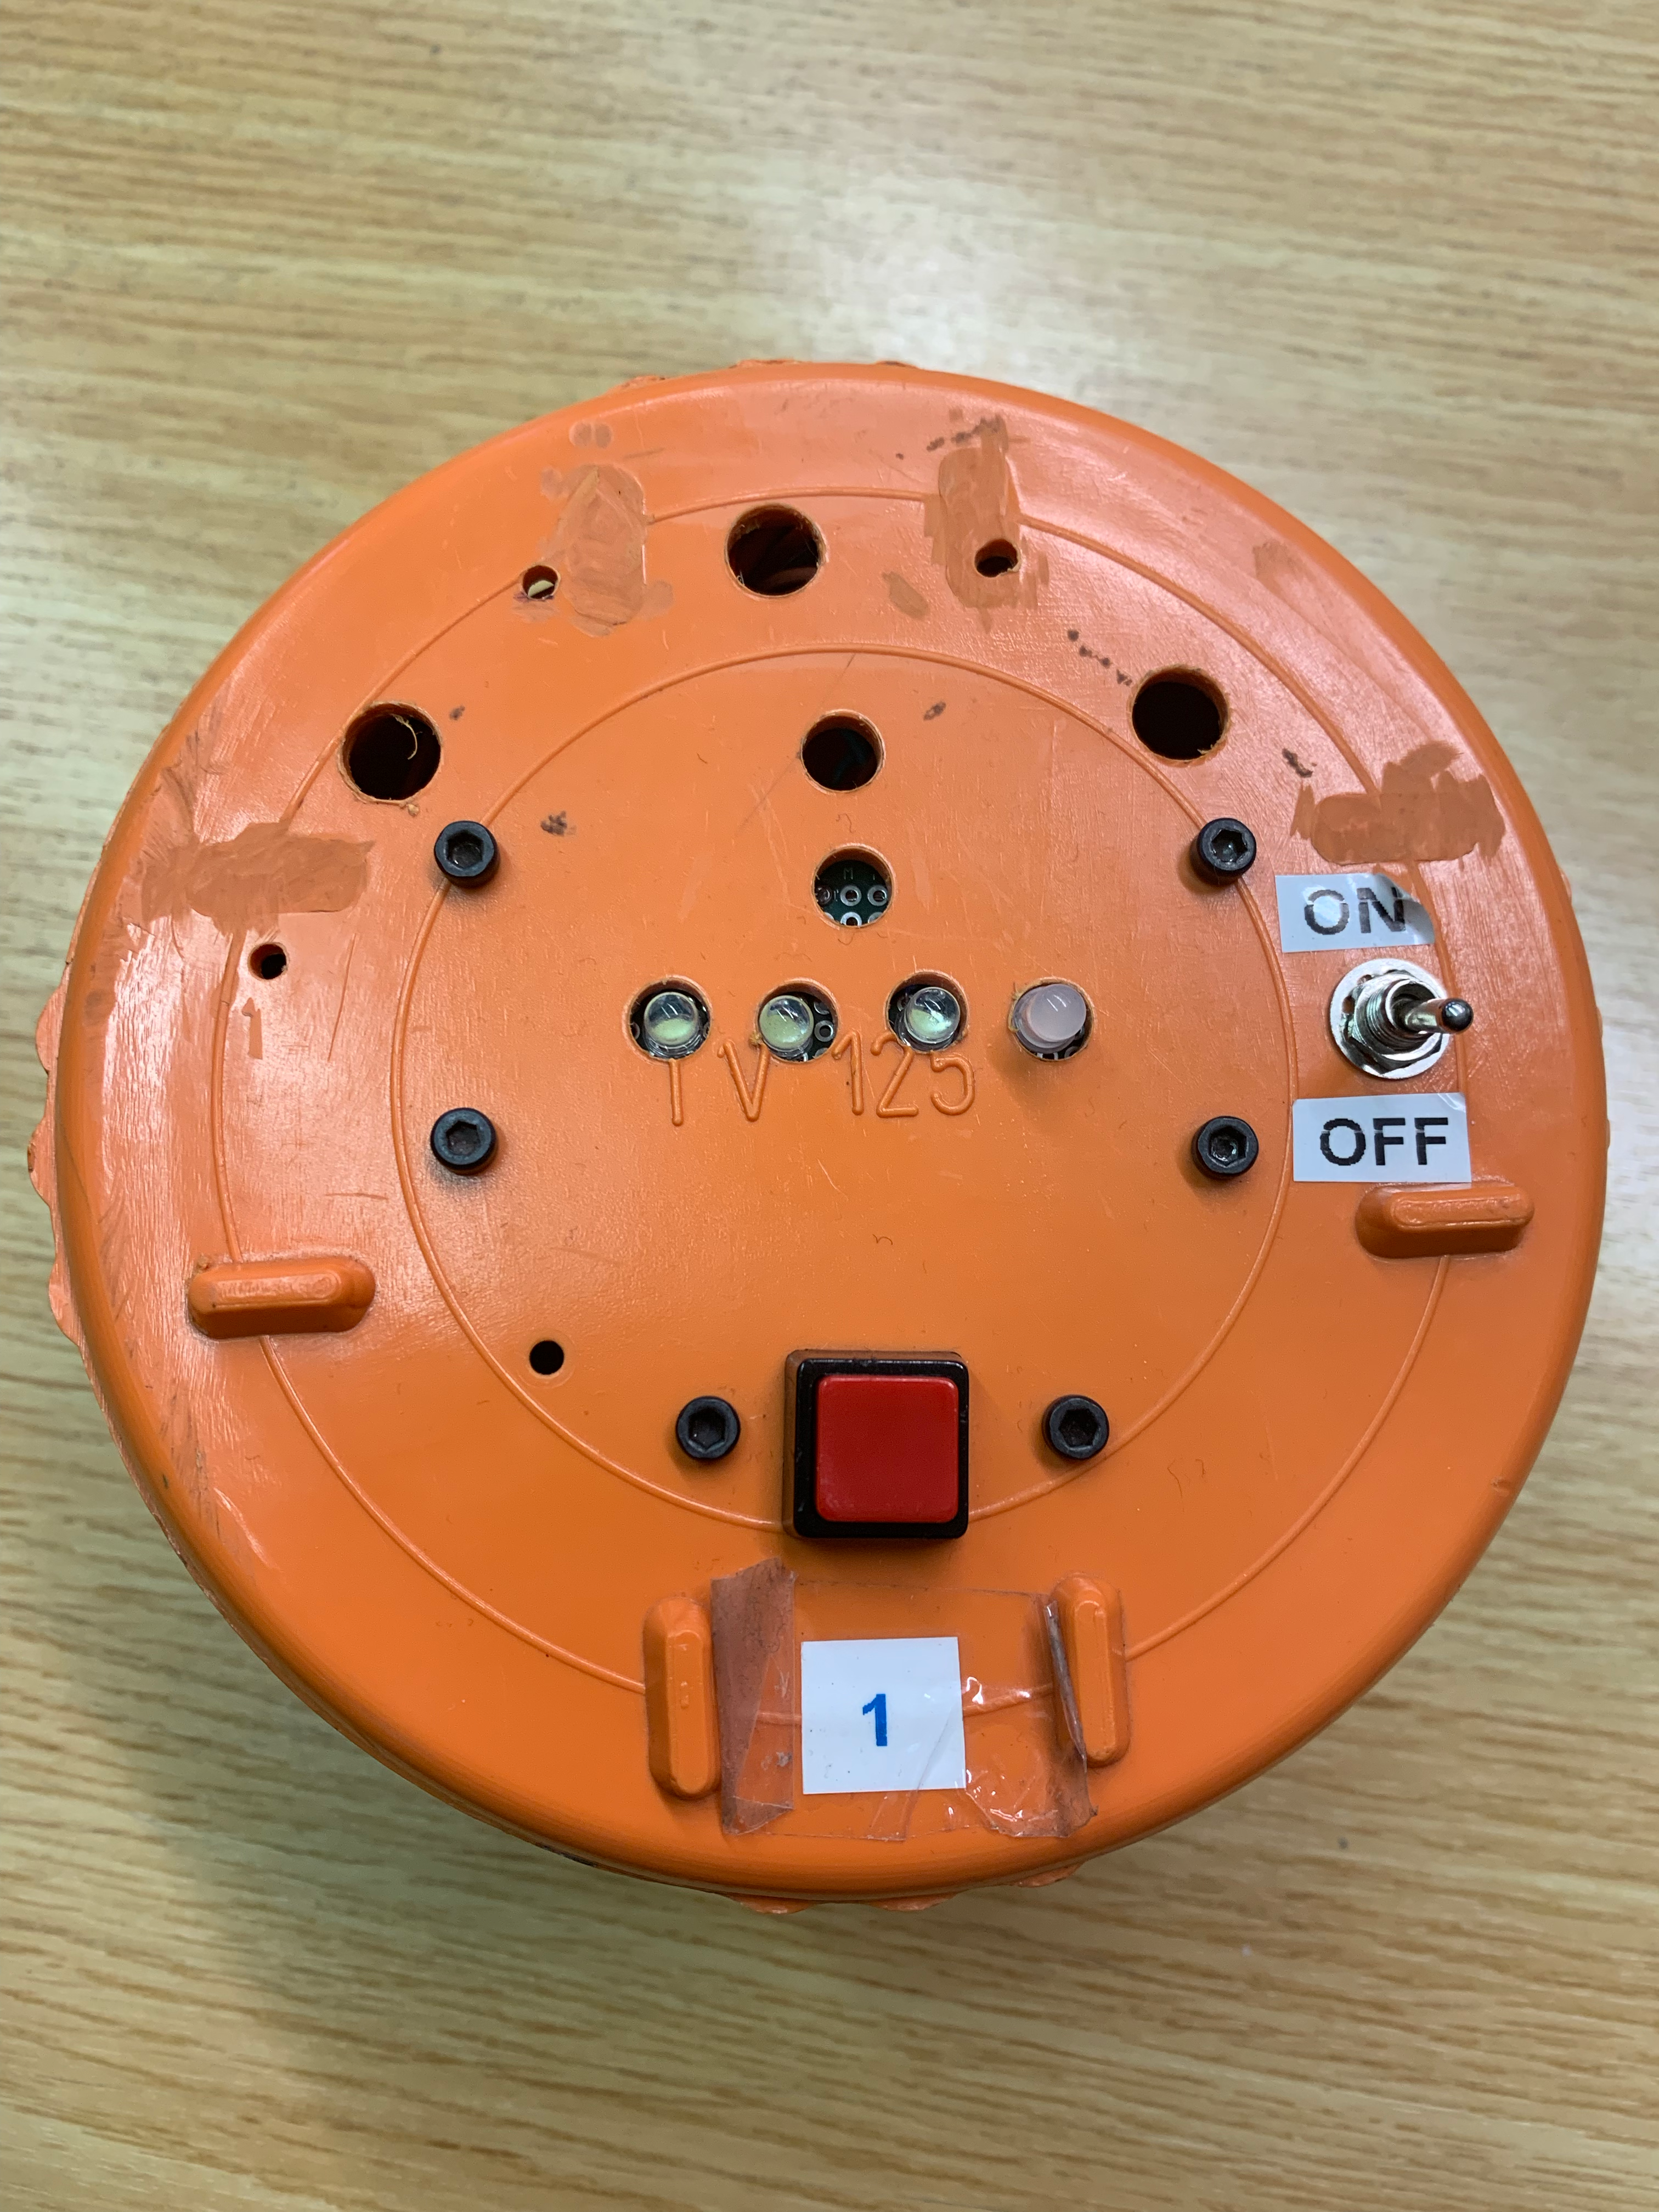
\includegraphics[width=3cm, height=5cm]{images/03-foundation/cap1}
	\caption{}
  \end{subfigure}
  ~ 
  \begin{subfigure}[t]{0.33\textwidth}
  	\centering
    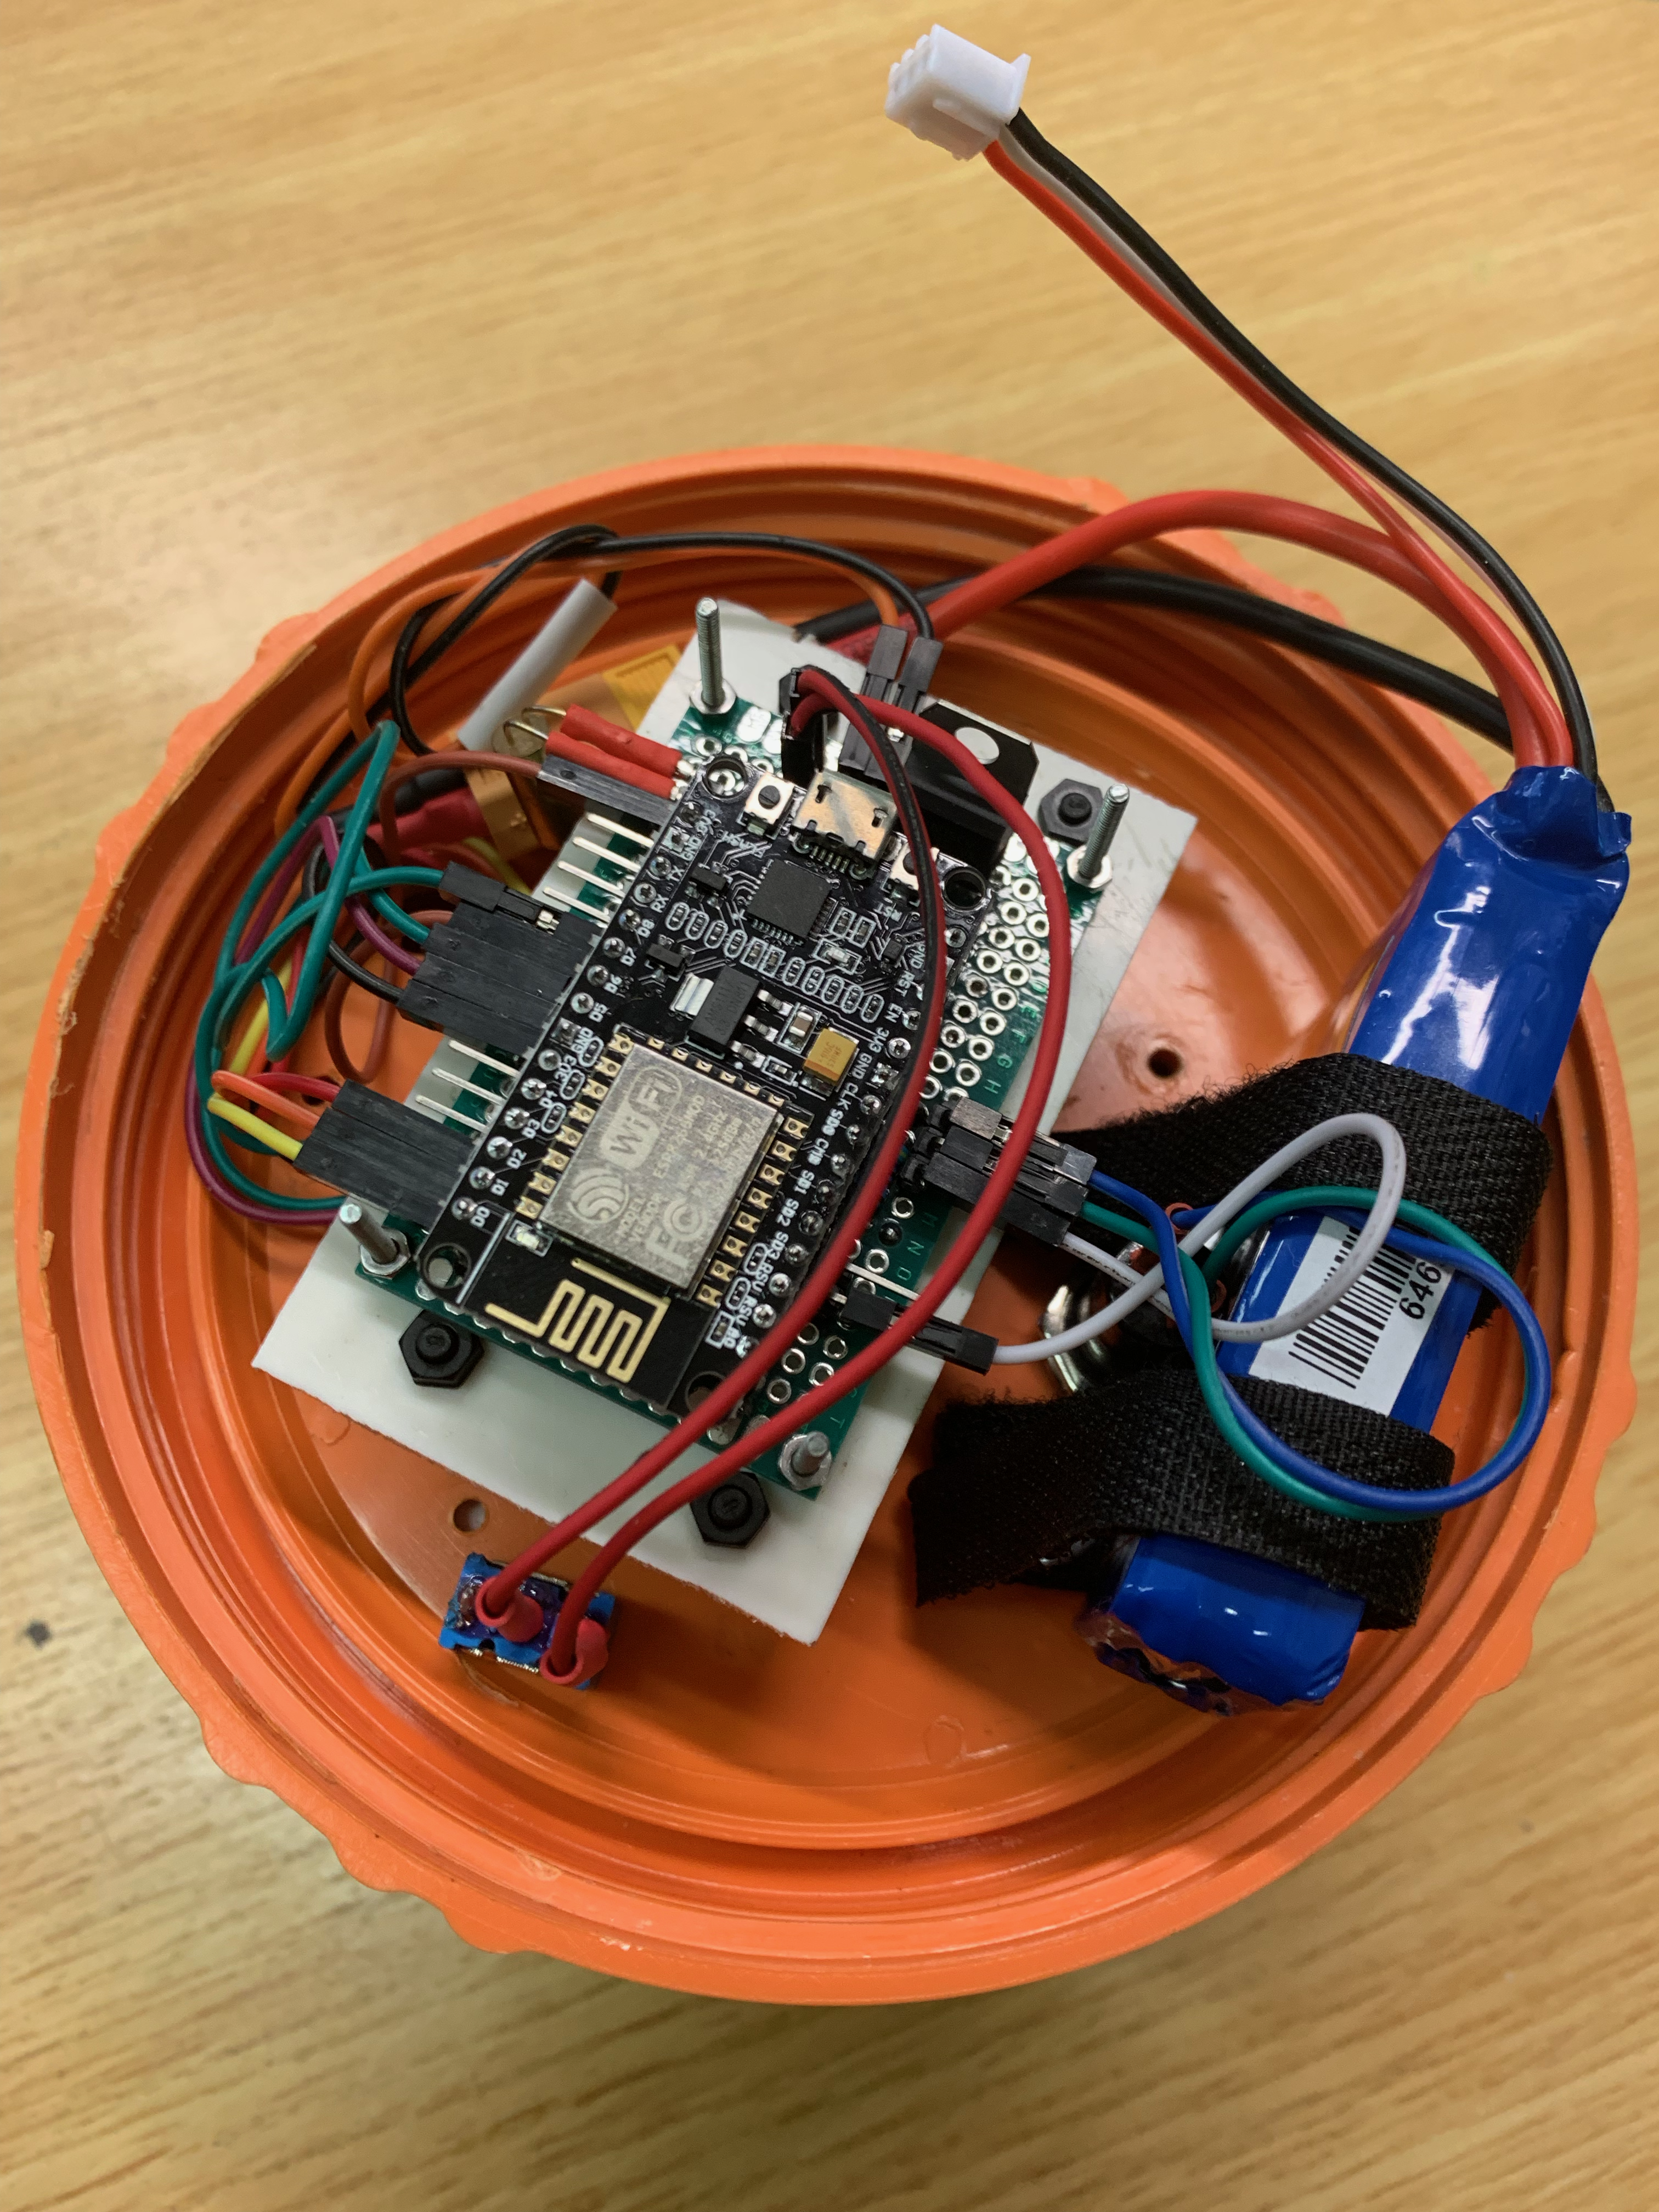
\includegraphics[width=3cm, height=5cm]{images/03-foundation/cap2}
	\caption{}
  \end{subfigure}
  ~
   \begin{subfigure}[b]{0.33\textwidth}
	  \centering
      \includegraphics[width=3cm,  height=5cm]{images/04-activity/tubes.jpg}
      \caption{}
    \end{subfigure}
  \caption{a) Tower cap containing the button and \gls{led}s; b) Tower cap circuit; c) The four towers used in the game (height 110cm).}
  \label{fig:tower_caps}
\end{figure}


\begin{figure}[H]
	\centering
		\includegraphics[width=0.4\textwidth, height=5cm]{images/03-foundation/tilt_sensor_circuit}
	\caption{The circuit for detecting when a tower has fallen. An angle switch detects the inclination and the low-pass filter smooths out noise from vibrations such as those caused by the player touching the tower. The signal wire is attached to a pin on the NodeMCU V3 ESP8266 ESP-12E WiFi Module, which allows communication with the robot's onboard computer.}
    \label{fig:tilt_circuit} 
\end{figure}

\section{The robotic platform}\label{sec:roboplat} 
As depicted in figure~\ref{graph:PIRG_design_structure}, hardware is the core concern for a mobile robot in~\gls{pirg}. In the graph in figure~\ref{graph:HARDWARE_structure} we have detailed some concepts of importance considered during our design. The graph is not supposed to give an extensive map of the necessary hardware aspects and their inter relationship, but to instruct the reader on the necessary aspect in this first phase of design taking our development as example. Naturally, not all mobile robots involved in~\gls{pirg}s will take into account all such concerns. In fact, the original RoboTower~\citep{bonarini_timing_2014} and Jedi Trainer 3.0~\citep{martinoia_physically_2013} were examples of mobile robots that did not considered, for instance, navigation techniques, such as~\gls{slam} and~\gls{oa} and had no sophisticated structural and sensing requirements given the little computing power available.

Our wheeled robot, instead, had holonomic kinematics and was called Triskar. Being holonomic, it was free to move in any direction at a speed comparable to that of people in indoor environments (up to 1.4~m/sec). The base consisted of a metallic, triangular-shaped structure where motors, batteries, computer and necessary electronics are embedded. In total, the robot weighed $22.3$ kg. Triskar had simultaneously and independently controlled rotational and translational motion capabilities thanks to three omni-directional wheels actuated by a motor each. The robot's movement on flat floor was as free as the human which made it a good base for adversarial~\gls{pirg}s and, in particular, the one that we had designed. 

\begin{figure}[H]
    \centering
    \begin{tikzpicture}[ every annotation/.style = {draw,
                         fill = white, font = \Large}, scale=0.75,transform shape]
                         
      \path[mindmap,concept color=black!40,text=white,
        every node/.style={concept,circular drop shadow},
        root/.style    = {concept color=black!40,
          font=\large\bfseries,text width=10em},
        level 1 concept/.append style={font=\Large\bfseries,
          sibling angle=90,text width=7.7em,
        level distance=15em,inner sep=0pt},
        level 2 concept/.append style={font=\bfseries,level distance=9em},
      ]
        node[concept, font=\fontsize{20pt}{17pt}\selectfont\bfseries] {Hardware}
        [clockwise from=0]
        child[concept color=blue] {
          node[concept] {Power}
          [clockwise from=-60]
          child { node[concept, font=\fontsize{7pt}{17pt}\selectfont\bfseries] {Consumption} }
          child { node[concept] {Capacity} }
        }
        child[concept color=black] {
            node[concept] {Computing}
            [clockwise from=10]
            child[concept] { node[concept] {Planning} }
            child[concept] { node[concept] {Tracking} }
            child[concept] {
                node[concept,scale=1.5,font=\fontsize{9pt}{17pt}\selectfont\bfseries] {Navigation}
                [clockwise from=250]
                child { node[concept, font=\fontsize{7pt}{17pt}\selectfont\bfseries] {SLAM} }
                child { node[concept, font=\fontsize{8pt}{17pt}\selectfont\bfseries] {OA} }
            }
            child[concept] {
              node[concept] {Sensing}
              [counterclockwise from=150]
              child { node[concept, font=\fontsize{7pt}{17pt}\selectfont\bfseries] {Range} }
              child { node[concept, font=\fontsize{7pt}{17pt}\selectfont\bfseries] {HZ} }
              child { node[concept, font=\fontsize{7pt}{17pt}\selectfont\bfseries] {Cost} }
              child { node[concept, font=\fontsize{7pt}{17pt}\selectfont\bfseries] {Proc} }
            }  
        }
        child[concept color=red] {
            node[concept] {Structure}
            [clockwise from=160, scale=0.8]
            child { node[concept, font=\fontsize{8pt}{17pt}\selectfont\bfseries] {Kinematics}}
            child { node[concept, font=\fontsize{8pt}{17pt}\selectfont\bfseries] {Material}}
            child { node[concept, font=\fontsize{8pt}{17pt}\selectfont\bfseries] {Robustness}}
            child { node[concept, font=\fontsize{8pt}{17pt}\selectfont\bfseries] {Safety}}
        };
    \end{tikzpicture}
    \caption{Some relevant concepts in the hardware dimension for the design of a~\gls{pirg} mobile agent. SLAM stands for Simultaneous localization and Mapping, a set of techniques related to navigation. OA stands for Obstacle Avoidance. Proc and Hz, under sensing, stand for Processing and Frequency respectively.}
    \label{graph:HARDWARE_structure}
\end{figure}

During the research progress, we have designed several versions of our robot, where the first two had an overall height of 85~cm, so comparable to that of a child players, but also acceptable for adult players. The first three versions adopted a Kinect\textsuperscript{\textregistered} sensor on top aimed at player tracking. Given the need to improve robustness, we have redefined the base by making structural changes to limit vibrations and improve stability of the sensors, which increased the overall height to 1 meter (2nd version). We also added new sensors such as planar laser scans needed to obtain reliable obstacle avoidance and localization (3rd and 4th version). Figure~\ref{fig:evolution} depicts our prototype evolution. Finally, on the fourth version we dropped the 3-D camera, deemed to be too much unreliable for player detection, and devised for this goal algorithms based on laser scans only. We kept the height in the same range as before, for the mentioned reasons, although it was no longer needed to hold Kinect\textsuperscript{\textregistered}. To justify the height and give a character to the robot, we added eyes and hair on top, which were appreciated by players. On the next section we expose some consideration regarding sensing.

\begin{figure}[H]
      \centering
      \begin{subfigure}[b]{0.22\textwidth}
      	\centering
	    \framebox{\parbox{2.5cm}{\includegraphics[draft=false,height=4cm,width=2.5cm]{images/03-foundation/triskar1}}}
	  	\caption{}
	  	\label{fig:evolution_a}
      \end{subfigure}
	 ~
	  \begin{subfigure}[b]{0.22\textwidth}
		\centering
	  	\framebox{\parbox{2.5cm}{\includegraphics[draft=false,draft=false,height=4cm,width=2.5cm]{images/03-foundation/triskar2}}}
	  	\caption{}\label{robot}
      \end{subfigure}
      ~
      \begin{subfigure}[b]{0.22\textwidth}
      	\centering
      	\framebox{\parbox{2.5cm}{\includegraphics[draft=false,draft=false,height=4cm,width=2.5cm]{images/03-foundation/triskar3}}}\label{newrobot}
      	\caption{}
      \end{subfigure}
      ~
      \begin{subfigure}[b]{0.22\textwidth}
	      \centering
	      \framebox{\parbox{2.5cm}{\includegraphics[draft=false,draft=false,height=4cm,width=2.5cm]{images/03-foundation/base4.png}}}\label{newrobot}
	      \caption{}
      \end{subfigure}
      \caption{Prototype evolution. a) First version having the Microsoft Kinect\textsuperscript{\textregistered} camera sensor support secured by steel cables in order to reduce vibration due to motion. b) Second version had improved stability by replacing the steel cables by rigid modular aluminum profiles. c) Third version had a completely redefined base including new electronics, thicker aluminum chassi, redesigned power distribution system and 2D lasers. This version also had a larger base compared to previous prototypes; d) Current version during demonstration at the Maker Faire 2018 in Rome (the European edition) from October 12th to 14th of 2018. A better placement of lasers had made the use of Kinect\textsuperscript{\textregistered} unnecessary since it allowed for full 360\textsuperscript{$\circ$} laser sensing coverage.}
      \label{fig:evolution}
\end{figure}

\subsection{Sensing}
\subsubsection{Microsoft Kinect\textsuperscript{\textregistered}\label{sec:kinectsec}}
In some phases of our development we have used the Microsoft Kinect\textsuperscript{\textregistered} sensor. It is a 3-D camera: in addition to providing an RGB image with its 1080p color camera, it also provides a depth map,  meaning that for every pixel of the depth image provided by the sensor, Kinect\textsuperscript{\textregistered} provides the distance from the sensor (see appendix~\ref{app:hard_appendix} for sensor specifications). This makes the it suitable for a variety of computer vision problems like background removal, blob detection, and people tracking.

\subsubsection{Laser scanners}\label{lasershokuyo}
The robot was equipped with two laser scanners Hokuyo URG-04LX\footnote{\url{https://www.hokuyo-aut.jp/search/single.php?serial=165} accessed on \today}
%, shown in Figure~\ref{fig:hokuyo}
. These laser sensors perceive the range of obstacles on a plan with a field of view of $240^\circ$ and a resolution of $0.36^\circ$, the maximum detectable distance is $5.6m$ and they can be connected to the computer by means of a USB interface, being operated with a nominal voltage of 5V.

The Hokuyo URG-04LX consists of a compact stacked structure with a spindle motor and the actual scanner on top of it. The motor rotates a small transmission mirror that deflects the vertical laser beam coming from the top of the sensor into horizontal direction. This allows the laser beam to scan a planar area around the sensor with an opening angle of $240^\circ$. A second mirror below, the reception mirror, deviates the horizontal laser beam captured by a lens into vertical direction again.

% \begin{figure}[H]
% 	\centering
% 	\includegraphics[width=5cm]{images/03-foundation/hokuyo}
% 	\caption{ An Hokuyo URG-04LX laser scanner.}
% 	\label{fig:hokuyo} 
% \end{figure}

A full scan is performed every 100 ms. We mounted a laser scanner on each side of the lower chassis allowing for a $360^\circ$ coverage around the robot at a height of 30 cm from the floor.

\section{Structure \& Materials}
\subsection{Chassis}
The chassis of our robot was made entirely from modular aluminum profiles put together as to define the shape in figure~\ref{fig:aluminum_structure} (3rd prototype). The arrangement of the wheels, as to allow for the holonomic behavior, also allowed us to place batteries conveniently~(see figure~\ref{fig:batteries}) as well as the onboard computer and electronics~(see figure~\ref{fig:computer}). The careful placement of heavyweight elements, such as the lead-acid batteries, turned out to be important in our design since it impacted manoeuvrability. For instance, during test it occurred that, due to inertia, the robot would become vertically unstable when making quick turns or rapidly reacting to the human player's presence. 

The constraint of having the Microsoft Kinect\textsuperscript{\textregistered} sitting on top of a aluminum profile, as to allow maximum visibility from the sensor, moved the center of mass upwards making vertical balance worse. The void created between the wheels, in prototype versions three and four, elegantly provided a way to balance weights and make the robot's center of mass close enough to its base center. Figure~\ref{fig:evolution_a} documents the inefficient weight distribution in the first prototype. In the figure its possible to see the placement of one of the lead-acid batteries in the right side of the base, thus, making the weight distribution asymmetric.

Due to forces acting upon the robot during motion we have used software solutions for velocity smoothing that would increasingly bound speed when accelerating and decelerating. This, together with a proper weight distribution, rendered the robot's motion smooth, improving control, at the benefit of reducing the chances of mechanical breakdown caused by material stress.

\begin{figure}[h]
    \centering
    \begin{subfigure}[b]{0.22\textwidth}
      	\centering
        \framebox{\parbox{2.5cm}{\includegraphics[draft=false, height=4cm,width=2.5cm]{images/03-foundation/structure}}}
        \caption{}
        \label{fig:aluminum_structure}
    \end{subfigure}
    ~
    \begin{subfigure}[b]{0.22\textwidth}
      	\centering
        \framebox{\parbox{2.5cm}{\includegraphics[draft=false,height=4cm,width=2.5cm]{images/03-foundation/structureII}}}
        \caption{}
        \label{fig:batteries}
    \end{subfigure}
    ~
    \begin{subfigure}[b]{0.22\textwidth}
      	\centering
        \framebox{\parbox{2.5cm}{\includegraphics[draft=false,height=4cm,width=2.5cm]{images/03-foundation/structureIII}}}
        \caption{}
        \label{fig:computer}
    \end{subfigure}
    \caption{Structural details of our robot. The chassis is made of modular aluminum profiles from which rapid and easy prototyping is possible while retaining a good level of robustness. a) The full scale view of the robot (3rd version). b) a close-up view of one of the 2-D lasers and batteries (gray boxes). c) a close-up view of the vertical placement of computer (black box) and control board (red board).}
    \label{fig:structure_details}
\end{figure}

\subsection{Kinematics}

\subsection{Power distribution}

\section{Computing}

\subsection{Onboard computer}\label{onboard pc}
For computing a Shuttle XPC Slim DH270 was used. The device has a $190 \times 165 \times 43$~mm steel case, and weights $1.3$~kg.  The armature presents two holes for Kensington Locks and numerous threaded holes (M3) at both sides allowing for an easy placement. The operating system used was~\textit{Ubuntu 16.04.3 LTS (64bit)}. The computer had an Intel Core i7 and a RAM DDR4 memory of 16 GB .

\section{Control boards}
\label{novacore}
The low-level motors actuation and their interface between the ROS system have been realized with the Nova Core modules based on STM32-chip~\cite{noauthor_nova_nodate}, which implement ready to use components to fulfill robot prototyping requirements with plug \& play approach.  
The provided modules allow to control different type of motors that can be modeled as a second order system, where the input is the voltage applied to the motor armature and output variable is the motor angular speed. Futher details about the deployed boards are presented in figure~\ref{fig:boards}.


\begin{figure}[H]
  \centering
  \begin{subfigure}[b]{0.3\textwidth}
  \centering
      \includegraphics[width=3cm,height=3cm]{images/03-foundation/udc}
	\caption{}
  \end{subfigure}
  \begin{subfigure}[b]{0.3\textwidth}
  \centering
      \includegraphics[width=3cm,height=3cm]{images/03-foundation/io}
	\caption{}
  \end{subfigure}
  \begin{subfigure}[b]{0.3\textwidth}
  \centering
      \includegraphics[width=3cm,height=3cm]{images/03-foundation/usb}
	\caption{}
	\label{fig:usb_board}
  \end{subfigure}
  \caption{a) UDC board (1 per each motor) capable of driving motors up to 70 W, with torque, speed, and position closed loop control. General attributes: 5-28V supply; 3A max (5A peak); current sense; encoder input; limit switch input; 25 x 45 mm in size. b) IO board (1 per each motor): Integrate existing hardware into the real-time Nova Core bus with analog and digital signals. General attributes: 8 digital GPIO;  4 analog inputs; 2 analog outputs; 2 UART; 1 I2C; 1 SPI; 25 x 45 mm in size. c) USB board (used for data collection) Interface the real-time Nova Core bus with a computer and logs data to microSD memory. General attributes: USB connector;  UART connector; microSD card slot; rosserial support; 25 x 45 mm in size.}
  \label{fig:boards}
\end{figure}
%ANDY all the technical details and names of devices could go in an appendix, while I'll leave here a functional description of robot and sensors, giving the characteristics that are functionally relevant, e.g., speed, omnidirectionality, range of sensors, their data rate, ...

\section{Navigation}
\subsection{\glsdesc{slam}}
\subsection{\glsdesc{oa}}

\section{Player perception and Tracking}
For opening the device, we have used libfreenect2\footnote{~\url{https://github.com/OpenKinect/libfreenect2} accessed on \today.}, a library for managing the Kinect\textsuperscript{\textregistered} device on Linux. We have then created a custom tracking node capable of estimating the player's position in two phases: First, color blob detection. Second, segmentation on the depth frame using \textit{region growing} algorithm for the purpose of detecting the player's body. Two features can be detected from this procedure: distance (relative to the robot) and contraction index. The first is calculated from the mean value of the depth pixels around the center of the blob. The latter is computed based on the subtraction of the occupied area with respect to the dimension of the bounding box that encompasses the segmented silhouette (see Figure~\ref{fig:segmenta}). This feature had been considered as a cue about the fact that the player was opening arms, so, possibly, actively participate to the game.

\begin{figure}[h]
  \centering 
  \begin{subfigure}[b]{0.3\textwidth}
		\centering
		\framebox{\parbox{3cm}{\includegraphics[draft=false,width=3cm, height=3cm]{images/03-foundation/point_cloud}}}
		\caption{}
  \end{subfigure}
  ~
  \begin{subfigure}[b]{0.3\textwidth}
		\centering
		\framebox{\parbox{3cm}{\includegraphics[draft=false,width=3cm, height=3cm]{images/03-foundation/depth}}}
		\caption{}
  \end{subfigure}
  ~
  \begin{subfigure}[b]{0.3\textwidth}
		\centering
		\framebox{\parbox{3cm}{\includegraphics[draft=false,width=3cm, height=3cm]{images/03-foundation/segmentation}}}
		\caption{}
  \end{subfigure}
  \caption{Example of frames processed by our algorithm. a) Point cloud showing the center of the detected (light-purple) color blob. b) Depth frame. The number showed above the user correspond to his estimated distance relative to the robot (in meters). c) Segmentation results. The number above is the contraction index defined in the interval [0,1] and can be used as a measure of body contraction.}\label{fig:segmenta}
   \label{segmentacao}
\end{figure}
\chapter{Exploring Activity Recognition in Robogames}

On a~\gls{pirg}, one is often interested in modeling the human player behavior and, from such modeling, program the system to respond properly. Our research began by exploring activity recognition and how that could be incorporated on the design of better~\gls{pirg}'s. 

In the literature, some approaches for activity recognition are based on the analysis of data coming from camera devices. Others, instead, focus on data coming from wearable devices, such as: cellphones, watches and~\gls{imu} -- a specific-purpose device for measuring accelerations and rotation angles. Across years, the type of analysis carried out has pretty much shifted from basic exploratory analysis,~\eg summary statistics, to complex data-based models, such as those from the~\gls{ml} community. The advantage of this is in the fact that~\gls{ml} models often grant better results by the characterization of the hidden structures present in data.

One may spot at least two groups into which to classify works in the area: those performed on an off-line manner and those performed on an on-line one. The first focus on the exploitation of methods for the case were data are first collected, tagged and them processed. The philosophy behind on-line methods, as the name suggests, rely on methodologies that can process the data on the go, providing real-time information about the estimated activity. In all of the vast literature in this field,~\gls{ml}-based approaches rely on some kind of transformation to the data in order to increase recognition results.

In the following, we present how we exploit a simple transformation of the input space targeting the creation of a flexible, generic, and well defined framework for activity recognition in a~\gls{pirg} scenario. To the best of our knowledge, our proposal is the first one to incorporate activity recognition on a~\glsdesc{pirg} involving a human and a mobile robot in a adversarial game setting.

\section{Introduction}

Detailed measurement and classification of an individual's physical  activity is fundamental in order to understand the relationship between physical activity and health but, also, to achieve an enhanced level of interaction between humans and robots. In particular, when considering~\glsdesc{pirg}~\cite{martinoia_physically_2013} -- where the objective is the exploitation of both the real world as environment, and of one or more real, physical, autonomous robots as game opponents or companions of human players -- activity recognition plays a fundamental role to adapt the robot strategy to support the player's entertainment during the game.

Here we propose a model which aims at classifying player's activity in a~\gls{pirg} game using a 3-axis custom accelerometer positioned on the player's chest. We define a set of high level activity classes that are automatically classified relying on a supervised machine learning framework. Our methodology consists of transforming the raw input space into one that is able to capture variance of the signal to emphasize the recognition of the target activities. 

Our main contribution is on the fact that we are able to obtain reasonable results in accuracy by applying a simple transformation. The achieved results are comparable, in terms of accuracy, with sliding window approaches, which makes our method feasible for real applications, but at lower cost regarding data processing. We test out methodology on activity recognition during a real robogame scenario~(see section~\ref{sec:game_environment}). 

The chapter is organized as follows: we first present some related works about activity recognition and classification; In section~\ref{datacollection} we explain how we collected data, while in section~\ref{activityanalysis} we provide the description of the activity model. The results are finally discussed in section~\ref{discussion}.

\section{Related Works}\label{relatedworks}

A number of recent studies have investigated activity recognition using one or more accelerometer placed in different parts of the body. In~\cite{ravi_activity_2005}, a well-cited paper in the activity recognition community, the authors have used a triaxial accelerometer worn near the pelvic region in order to classify eight different daily-life activities: \textit{standing}, \textit{walking}, \textit{running}, \textit{climbing up stairs}, \textit{climbing down stairs}, \textit{sit-ups}, \textit{vacuuming}, and \textit{brushing teeth}.

%The feature extraction from the raw accelerometer data used the \textit{sliding windows} method, a very common stream processing method found in many applications. It consists in the process of making computation on a batch of data, called a windows, that is eventually updated with new incoming data. This update process is referred the``sliding of the windows''. When slided, the windows may retain some of the previous update data points, this is referred to the amount of \textit{overlap} used on the windows. 

The windows size used had 256 data-points with 128 samples overlapping ($50\%$ overlap) between consecutive windows. At a sampling frequency of 50Hz, each window represents data for 5.12 seconds. The ammount of overlap used is justified by the work of~\cite{bao_activity_2004}, where they had demonstrated the feasibility of such overlap. 

%~\cite{mannini2013activity} proposes daily physical activities recognition using a single accelerometer placed at the wrist or ankle. This study uses various combinations of window lengths and feature sets to develop an algorithm with the aim to classify a wide variety of activities into four distinct classes using accelerometer raw data and, also, higher classification accuracies for ankle data w.r.t the wrist data.

%These windows can be either fixed in size by including only the most recent n data points or by showing only the most recent t time units of data (where n and t are constants). While the implementation of this model is very simple, it is prone to errors when choosing a wrong window width. Too narrow windows will produce very accurate representations of the current state, but are heavily affected by noisy data while too wide windows result in more stable yet equally inaccurate results due to the effects of concept drift [2]. Nevertheless, fixed sliding windows can be found in many applications. An example is [7] where they are used to detect regions of abnormal network activity.

%The possibility of performing human activity recognition using raw accelerometer data from smart-phones is also a very common field of study. For example, in~\cite{bayat2014study} an experiment where subjects were requested to perform two different activities has been performed and, given their start and end times, two datasets were considered: one for in-hand phone position and one for in-pocket phone position. This information was then used to label different activities for a supervised learning classification problem. Another similar work was~\cite{anguita2013public}, while in~\cite{su2014activity} a number of applications for such studies are also proposed. %%% EWERTON: This paragraph is strange, it has to give some it doesn't give much information about the studies. The last sentence just mentions papers but doesn't present their goals or methodology. It has to be changed. %%%

Considering a game environment,~\cite{jablonsky_evaluating_2017} investigated sensor placement and modality for activity recognition within the context of children's playground  activities. By mean of parallel sensing, performed using a set of smart-phones, activity dependent data have been generated. The obtained set of data was then used to train decision tree classifiers. This study shows once again that phones placed closer to the core of the body generate better models than phones placed on the  extremities. 

Similarly, in~\cite{alshurafa_designing_2014} a stochastic approximation framework for intensity independent activity recognition based on clustering techniques is proposed. The aim is to enhance and automate the calculation of~\gls{met} and also to improve an exergaming (video games that are also a form of exercise) platform consisting of two main components: an accelerometer-embedded belt and an~\gls{rpg} video game called \textit{FreedroidRPG} that was used as an incentive for the participant to perform physical activity throughout the day. The study shows the ability of the used stochastic approximation framework to extrapolate unknown intensity levels from a few  known ones that can be used to enhance activity recognition.

Several studies in literature also focused on the comparison between multi-sensor versus single-sensor activity detection and also on the optimal body placement of such sensors.

The work of~\cite{gao_evaluation_2014} compared two distinct types of wearable systems: single-sensor wearable systems adopting complex algorithms and multi-sensor systems employing light-weight algorithms. The impact of the sampling rate on the recognition accuracy was then investigated using four classifiers. The experimental results illustrated that the recognition accuracy was steady at 50-Hz and above, and the single sensor system was more sensitive to the sampling rate than the multi-sensor system.

The work of~\cite{trost_machine_2014} is, in turn, focused on making a comparison between the activity recognition rates of an activity classifier trained on acceleration signal collected on the wrist and hip. During the experiments 52 children and adolescents completed 12 activity trials that were categorized into 7 activity classes: \textit{lying down}, \textit{sitting}, \textit{standing}, \textit{walking}, \textit{running}, \textit{basketball}, and \textit{dancing}. As result, the hip model exhibited great classification accuracy for \textit{sitting}, \textit{standing}, \textit{walking}, and \textit{running}; acceptable classification accuracy for \textit{lying down} and \textit{basketball}; and modest accuracy for \textit{dance}. The wrist model, in turn, exhibited excellent classification accuracy for \textit{sitting}, \textit{standing}, and \textit{walking}; acceptable classification accuracy for \textit{basketball}; and modest accuracy for \textit{running}, \textit{lying down} and \textit{dance}.

The present work, follows the line of reasoning present in popular one, such as~\cite{ravi_activity_2005, bao_activity_2004}, where the methodology relies on the use of supervised learning methods, powered by the extraction of discriminative features from a sliding window. However, the use of such method in our application scenario rises same special issues: since the annotated data come from real game interaction between a human and a mobile robot, the activities are not limited in any aspect.

Additionally, when using a traditional sliding window method, special attention has to be made on the choice of window size. This is because while a too narrow window will produce very accurate representations of the current state, it will also be heavily affected by noise. On the other hand, a too wide window results in more stable, yet similarly inaccurate results due to the effects of change in the underlying data~\cite{bifet_learning_2007}. 

Equally concerning, fixed-size windows are likely to ignore differences in the duration of activities. This happens very often in our scenarios where different in-game situations would make the players react differently. For instance, the time the player spends running are a product of multiple factors, including personal motivations and robot state given in-game situation. 

This would demand adaptive strategies for using sliding windows, as suggested by~\cite{noor_adaptive_2016}. However, in this work we follow a different route, by proposing to perform activity recognition by first transforming the data stream input space (acceleration raw data) into a different space that would capture the ``turbulence'' of the signal underlying each activity of interest %(standard deviation of the accelerations along xyz axis) - DAVIDE%. 
The motivation is that a running activity, for example, would be categorized by a different amount of turbulence compared to other activities.
%,such as simply standing or locally moving. - DAVIDE%
\section{The Game Scenario}\label{gamescenario}
In order to test our model, we designed a competitive game, where the human player faces an autonomous robot.

\subsection{The Robotic Platform}\label{roboplat} 
We have adopted a holonomic robot that is free to move in any direction at a maximum speed comparable to that of people in indoor environments (1.4 m/sec).

\begin{figure}[thpb]
    \centering
    \begin{subfigure}[b]{0.3\textwidth}
        \includegraphics[width=3cm,height=3cm]{images/04-activity/mobilerobot.jpeg}
        \caption{the robotic platform.}
    \end{subfigure}
    \begin{subfigure}[b]{0.3\textwidth}
        \includegraphics[width=3cm,height=3cm]{images/04-activity/tubes.jpg}
        \caption{the target tower used in the game (height 110cm).}
    \end{subfigure}
    \caption{}
    \label{fig:robot_tubes}
\end{figure}

The robot body consists of a robust, triangular, omni-directional base 5cm high (with 40 cm in diameter), where motors, batteries and electronics are embedded. On the base, an auxiliary aluminum structure is mounted, having the on-board computer attached laterally and a Kinect sensor on top. In total, the robot is 85cm high (see figure~\ref{fig:robot_tubes}).

\begin{figure}[thpb]
      \centering
      \includegraphics[width=3cm,height=3cm]{images/04-activity/sender.jpg}
      \caption{a) the custom accelerometer device used for human motion extraction based on Arduino Uno and a MPU-6050 breakout board. The data is transmitted to a receiver Arduino via Nrf24l01 radio frequency board.}\label{the_accelerometer}
\end{figure}

\subsection{Game Scenario}
For the present work, the ``playground'' is a rectangular area of 4m$\times$2m where, on each corner, ``towers'' are placed. Each tower is equipped with a button and four LEDs that can be progressively turned on, one by one, by pressing the button on the tower top. Each LED requires the button to be pressed for about 2.5 seconds, meaning that the tower takes about 10 seconds of button push in order to light up all of the four LEDs. Button pressing time is cumulated and can be distributed on different moments. After turning on all LEDs of a particular tower during game play, it is said that the player has captured it.

In order to win, the human player must be able to secure all the existing towers without letting a single one be ruined down by the robot. If, at anytime, a tower falls (because of the robot or player) the game ends and the human player is defeated. 

The robot is a holonomic base (see Figure~\ref{robot}(a)). It is able to move across the entire playground just as the human player and is only constrained by the fact that an already captured tower, or one whose button is currently pressed by the player cannot be teared down. The player can also block the robot path by staying in front of it. Notice that while the player is trying to capture a given tower, the robot can try to put down another one.

The robot must avoid hitting the player at any time during the game. Figure~\ref{robot}(b) presents the towers that were used in the game.

This game is designed so that the robot, given its agility and maximum speed (1.4 m/sec) could always win, but it should show the appropriate and believable behavior to keep the player engaged and interested.
  
\section{Method}

%before the activity analysis section shouldn't we put the data collection section? I think that in this way the explanation keeps its flow and everything it's more readable. Also a reviewer asked us to have a method section with the following subsection: hardware, data collection, feature extraction  -  DAVIDE%  

\subsection{Activity analysis}\label{activityanalysis}

On our game, by using an accelerometer attached to the player, we were mainly interested on identifying activities that would help to describe the player interaction level. For the scope of this work, we aimed at identifying recurrent physical activities that would be useful for achieving that goal. From the collected data (see section~\ref{datacollection}), we were able to identify a few high-level activity types, listed below:

\begin{itemize}
\item  \textbf{running:} describes a running activity. For this paper, multiple styles of running are not considered. For instance, ``fast'' or ``slow'' running are considered as the same.
\item \textbf{walking/dodging:} represents the walking and dodging activity. The latter refers to a sudden quick movement to avoid the robot or to call its attention.
\item  \textbf{locally\_moving:} a player generic motion that is too small to fall into other categories, but not so small to be characterized as inactivity. Robot path-blocking motions also fall into this type of motion.
\item  \textbf{inactive:} motion that are too low in intensity to be characterized as one of the above activities. A crisp threshold is used to delimit this category. 
\end{itemize}

By inspecting the data, we observed that a given player activity would occur in ``bursts'', being followed by a short period of inactivity (or rest), i.e., a short period where the player is not really moving, or the expressed acceleration motion is too small to be related to any fundamental activity of interest.

Resting periods are a common characteristic present in any physical game, both related to the organic human need for resting after an intense physical activity or even during strategic moments of pause. Examples of that can be seen when the player is pushing a button on a tower, or is trying to block the robot's path or is even waiting still for a specific robot position on the environment.

Naturally, on such moments of inactivity, the changes in acceleration are usually small, which produces a relative flatness of the signal (e.g., secs 9-12 and 15-18 on figure~\ref{acc_graph}) and allows for the delimitation of an activity begin/end time.

\begin{figure}[h!]
      \centering
      \includegraphics[width=\linewidth]{images/04-activity/newGraph.eps}
      \caption{Graph of acceleration in x, y and z axis for a game that lasted about 40 seconds.}
      \label{acc_graph}
\end{figure}

One way to describe the activity information carried on by the acceleration patterns is by considering the amount of signal ``turbulence''. As a measure of such turbulence, we rely on the information present on the signal variance. 

For this, we process the incoming data stream by computing the standard deviation of the signal inside a sliding window. This transforms the original input space into a new space where activity information are much easily seen: resulting in the generation of a continuous graph, where pulses refer to a given player's physical activity (see figure~\ref{std_graph}). % Also, in my opinion, this analysis is still representative without being affected by the noise coming from the accelerometer's signal so it's feasible also for cheap devices that cannot guarantee a great measurement accuracy. Do you think is the case to say this? - DAVIDE%

Working this way turns out to be simpler than to perform data annotation by, for instance, using a predefined sliding windows size. In our case, activities, such as ``running'', do not have fixed time duration, which makes the applicability of fixed sliding windows methods not well suitable~\cite{noor_adaptive_2016}.

\begin{figure}[thpb]
      \centering
      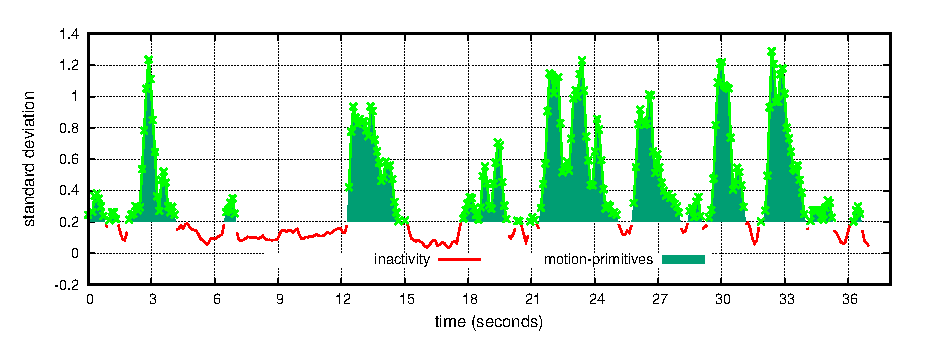
\includegraphics[width=\linewidth]{images/04-activity/newStdGraph.eps}
      \caption{Standard deviation of the acceleration in Figure~\ref{acc_graph}, computed using a sliding window of half a second. The red line portions represent variance values inside the inactivity zone (below a threshold of 0.2). Green areas are referenced as ``motion primitives''.}
      \label{std_graph}
\end{figure}

After performing the mentioned data transformation, we have empirically identified a crisp threshold that would catch irrelevant signal values, thus, we say that any value below that threshold is related to player's inactivity.
% for the sentence above maybe we should say : from data analysis we have EMPIRICALLY determined a crisp threshold (a reviewer asked us to better explain why we choose to set the threshold to 0.2 and the word EMPIRICALLY is enough self explanatory... I think) -  DAVIDE % <-- EWERTON: THE FOLLOWING PARAGRAPH IS ENOUGH FOR THAT!
The inactivity threshold is game-dependent and sensitive to the position of the accelerometer as well. On our experiments, the selection of the inactivity threshold is done manually, via inspection of video recorded during the game.

\begin{figure}[thpb]
    \centering
    \begin{subfigure}[b]{0.3\textwidth}
     	\centering
        \includegraphics[width=3cm,height=3cm]{images/04-activity/enricorun.png}
        \caption{Player performing a running activity.}
	\end{subfigure}
    \begin{subfigure}[b]{0.3\textwidth}
     	\centering
        \includegraphics[width=3cm,height=3cm]{images/04-activity/run1.png}
        \caption{Associated running motion primitive.}
	\end{subfigure}
    \label{running}
\end{figure}

\begin{figure}[thpb]
  \centering
  \begin{subfigure}[b]{0.3\textwidth}
      \includegraphics[width=3cm,height=3cm]{images/04-activity/enricostill.png}
      \caption{Player performing local movements. }
  \end{subfigure}
  \begin{subfigure}[b]{0.3\textwidth}
      \includegraphics[width=3cm,height=3cm]{images/04-activity/still.png}
      \caption{Associated motion primitive.}
  \end{subfigure}
  \label{localmov}
\end{figure}
    
Since any motion information below the threshold is used to determine the ``inactivity'' of the player, we use machine learning-based classification only on each data interval above the threshold. This interval is called a ``motion primitive'' (Figure~\ref{std_graph}). The motion primitives are the data aggregations to which we associate a class label in the annotation procedure. 

Following the classification need, we have extracted the following descriptors from the motion primitives (recall, they refer to standard deviation of the raw values): 

\begin{itemize}
\item \textbf{mean}:  the mean values.
\item \textbf{activity\_time}: the time duration in seconds.
\item \textbf{max\_peaks}:  the max peak.
\item \textbf{number\_of\_peaks}:  the number of peaks.
\item \textbf{mean\_of\_peaks}: the mean of all peaks.
\item \textbf{max-min}: difference between max and min.
\item \textbf{std}: standard deviation.
\item \textbf{mad}: median absolute deviation.
\item \textbf{sma}: signal magnitude area.
\item \textbf{energy}: the signal energy.
\item \textbf{iqr}: interquartile range.
\item \textbf{mean\_over\_max}: mean of peaks divided by the max peak.
\item \textbf{maxInd}: index of the frequency component with largest magnitude.
\item \textbf{meanFreq}:  weighted average of the frequency components to obtain a mean frequency.
\item \textbf{skewness}:  skewness of the motion primitive.
\item \textbf{kurtosis}:  kurtosis of the motion primitive.
\item \textbf{freq-skewness}: skewness of the frequency domain signal.
\item \textbf{freq-kurtosis}: kurtosis of the frequency domain signal.
\item \textbf{pse}: Power spectral entropy.
\item \textbf{rms}: Return the root mean square.
\end{itemize}

%\begin{figure*}[!t]
% ensure that we have normalsize text
%\normalsize
%      \centering
%      {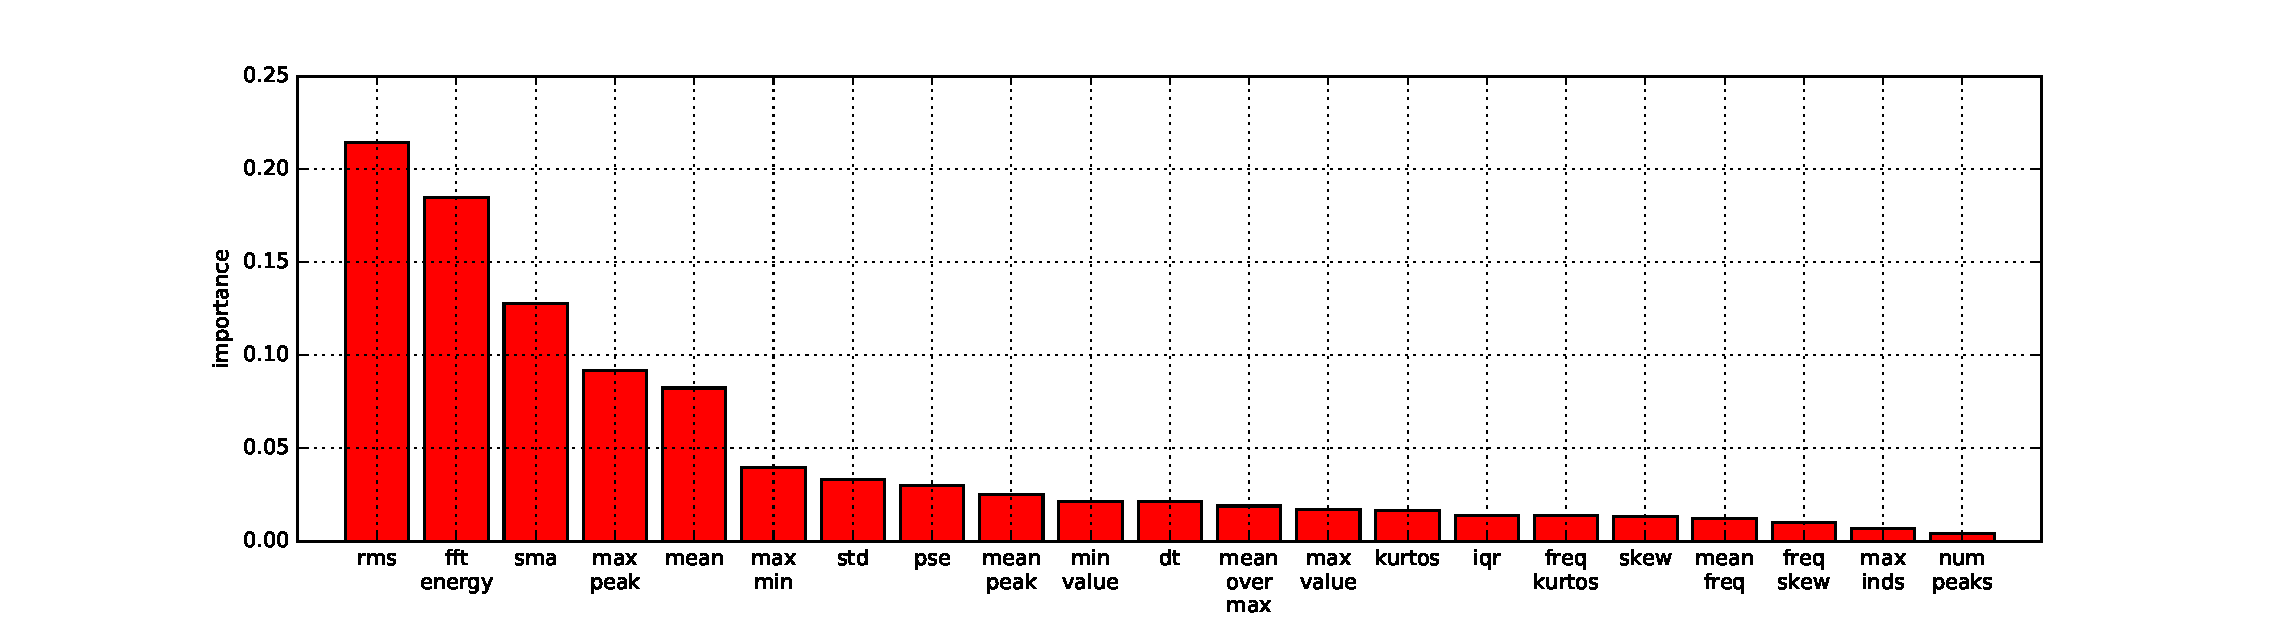
\includegraphics[width=\textwidth]{figures/featureImportance.eps}}
%      \caption{Feature importance computed by a forest of decision trees classifiers.}
%      \label{feature_importance}
%\end{figure*}

Note that, the motion primitives carry sufficient information to distinguish between target physical activities. For example, ``running'' is related to a motion primitive that has a longer duration and a higher amplitude value (see figure~\ref{running}) as opposed to the duration and amplitude values of a player local motion (figure~\ref{localmov}). Following the same argument, a ``walking'' activity has higher amplitude values compared with a local movement. A holistic view of the classification approach is detailed in Figure~\ref{approach}. 

\subsection{Data Collection}\label{datacollection}

When playing the game, we ask the human player to wear a colored robe (see figure~\ref{game}) in order to allow for blob detection and tracking, leading to feature extraction. The visual features extracted in the game are out of the scope of this paper, since we describe only results relying on the accelerometer data.

We have used a custom accelerometer board attached to the player's chest in order to capture a detailed player motion information. The device is based on the InvenSense MPU-6050 3-axis accelerometer board and an Arduino Uno micro-controller. The circuit also contains a Nrf24l01 radio-frequency module that allows the accelerometer data to be sent to the on-board computer. Figure~\ref{the_accelerometer} shows the accelerometer used.

The choice of the accelerometer position was conditioned by the need to minimize the influence of noise from irrelevant player motion.

\begin{figure}[thpb]
      \centering
      {\includegraphics[width=8cm]{images/04-activity/event.jpg}}
      \caption{Human player (in magenta) during the game. The playground configuration consisted of 3 target towers.}
      \label{game}
\end{figure}

For example, because the state of the towers are transmitted to the robot via radio frequency, it is not necessary to identify any related tower activity by means of acceleration patterns. Therefore, having the device placed on the wrist, or other highly movable body-part (as the feet or head) would capture useless acceleration information contributing to a decrease in classification accuracy for the mentioned target motions. 

In terms of collected data, for this work, we considered 29 matches involving 15 male participants of different ages. The age distribution consisted of children (7-10) and adults (26-40). Matches had a minimum time duration of about 40 seconds and a maximum of about 1 minute and 10 seconds. 

The collected data correspond to acceleration values along x, y, and z axis with a sampling frequency of 50Hz, which is five times larger than the frequency considered to be sufficient for detecting daily activities from accelerometer data (10Hz)~\cite{atallah_sensor_2010, ravi_activity_2005, kikhia_analyzing_2014}.

\begin{figure*}[!t]
\normalsize
      \centering
      {\includegraphics[width=\textwidth, height=4cm]{images/04-activity/diagram.png}}
      \caption{Overview of the activity recognition system.}
      \label{approach}
\end{figure*}

\subsection{Classification setup}

As pointed out, for the automatic classification we first build the standard deviation graph from the raw accelerometer data, and then we manually label motion primitives. 

On our experiments, the std graph was generated considering a sliding window 500msec long, resulting on a dataset composed by $367$ motion primitives with $34\%$ labeled as ``locally\_moving''; $25\%$ as ``walking/dodging'' and $41\%$ as ``running''.% and the others? would say a reader - ANDY

Empirically, this time length turned out to be descriptive enough to produce variance intervals that made it possible to distinguish activities. Naturally, the windows size has an impact on the total number of motion primitives generated per game match, as well as on the inactive threshold value. With a windows size of half a second, however, it was possible to capture immediate transition between activities, given that such transition would manifest on higher spikes on variance at the beginning of an activity. For that reason, we kept the mentioned size. 

As argued above, the ``inactive'' type is not considered in the recognition task since it is directly classified by the inactive threshold. From video log inspection, we observed that most of the useless motion would occurs below a threshold of $0.2$. 

Before training classifiers, we performed feature selection by evaluating the importance of the extracted features (see section~\ref{activityanalysis}) using random forest method, composed by 300 decision trees.% (see Figure~\ref{feature_importance}).

\section{Results and discussion}\label{discussion}

We tested different classifiers using 10-fold cross validation in order to have a more descriptive accuracy information. Following common practice, the train-test dataset ratio was defined as 80\% and 20\% respectively.

\begin{table}[h]\footnotesize
  \centering
  \caption{Cross-validation accuracy results for several classification methods using the 5 most significant features.% show in Figure~\ref{feature_importance}.
  }
  \begin{tabular}{| c | c |}
    \hline
  	   \textbf{Method}          & \textbf{Accuracy}\\\hline
       SVM (Linear Kernel)      & 0.80 (+/- 0.08)  \\\hline
       Random Forest            & 0.81 (+/- 0.06)  \\\hline
       Gaussian Naive Bayes     & 0.80 (+/- 0.11)  \\\hline
       Ensemble (Hard voting)   & 0.82 (+/- 0.10)  \\\hline
       AdaBoost                 & 0.65 (+/- 0.40)   \\\hline
  \end{tabular}
  \label{accuracy5best}
\end{table}

\begin{table}[h]\footnotesize
  \centering
  \caption{Classification report for the chosen ensemble method (Random Forest)}
  \begin{tabular}{| c | c | c | c | c |}
    \hline
  	   & precision   & recall & f1-score &  support \\\hline
    LM &      0.88   &  0.91  &    0.89  &      23  \\\hline
    WD &      0.79   &  0.60 &     0.68 &       25  \\\hline
     R &      0.77   &  0.92 &     0.84 &       26  \\\hline
avg/total &   0.81   &  0.81 &     0.80 &       74  \\\hline
  \end{tabular}
  \label{report}
\end{table}

Table~\ref{accuracy5best} presents 10-fold cross validation results using different classifiers on the five most important features, that is: \textit{rms}, \textit{fft\_energy}, \textit{sma}, \textit{max\_peak} and \textit{mean}. 

The ensemble in Table~\ref{accuracy5best} is defined as a majority (Hard) voting approach by the combination of the SVM, Gaussian Naive Bayes and Random Forest. The Adaboost method, in turn, takes a combination of 100 weak classifiers (Decision Trees). All methods were trained by using Python Scikit-learn machine learning library.

Despite the effort, with a confidence interval of 95\% we see that SVM, Random Forest, Gaussian Naive Bayes as well as their ensemble have a similar accuracy result. By considering the variance in their result, we see that Random Forest gives the most stable result. 

Given the 10-fold cross validation results, we decided to use as final method the Random Forest ensemble classifier (10 decision trees). Detailed results for the method are shown in table~\ref{report} and the corresponding confusion matrix and Receiver Operating Characteristic in Figure~\ref{mtx-roc}. The majority of mistakes in the classification correspond to the difficulty in separating ``walking/dodging'' from  a ``running'' activity. 

The justification for this may be on the fact that occasionally the player walks in a fast way what causes an increase in similarity with proper running. This is acceptable given that even for humans it is not straight forward to decide about the boundaries conditions of two different but related activities.

Despite the fact that our method relies on the computation of a fixed slide window when transforming the input data, we see that our method also allows for a small improvement in the annotation procedure. Consider, for example, that we do not have to worry about the effects of overlapping windows. Things like the choice of windowing functions, which are used to mitigate the effects of overlap, are not needed. Also, it allows for a more intuitive way of perceiving what underlying activity has occurred.

We have already conducted experiments on using our method online, and the results have been satisfactory. One drawback, however, is on the possibility of having two different activities associated to the same motion primitive. This is likely to occur when the player rapidly shifts between two activities. For exampl, this happens when the player stops running for a fraction of a second and then immediately starts walking. In that case we see a small decrease in the signal variance that may not be enough to characterize an inactivity period. Note that a value below the inactive threshold is the event that separates motion primitives.

\begin{figure}[thpb]
    \centering
    \begin{subfigure}[b]{\textwidth}
       \centering
       \includegraphics[width=12cm]{images/04-activity/conf_mtx.eps}
       \caption{Confusion matrix for the trained Random Forest ensemble method and the associated.}
	\end{subfigure}
    \begin{subfigure}[b]{\textwidth}
     	\centering
        \includegraphics[width=12cm]{images/04-activity/roc.eps}
        \caption{ROC curve.}
	\end{subfigure}
    \label{running}
\end{figure}

% An example of a floating figure using the graphicx package.
% Note that \label must occur AFTER (or within) \caption.
% For figures, \caption should occur after the \includegraphics.
% Note that IEEEtran v1.7 and later has special internal code that
% is designed to preserve the operation of \label within \caption
% even when the captionsoff option is in effect. However, because
% of issues like this, it may be the safest practice to put all your
% \label just after \caption rather than within \caption{}.
%
% Reminder: the "draftcls" or "draftclsnofoot", not "draft", class
% option should be used if it is desired that the figures are to be
% displayed while in draft mode.
%
%\begin{figure}[!t]
%\centering
%\includegraphics[width=2.5in]{myfigure}
% where an .eps filename suffix will be assumed under latex, 
% and a .pdf suffix will be assumed for pdflatex; or what has been declared
% via \DeclareGraphicsExtensions.
%\caption{Simulation Results}
%\label{fig_sim}
%\end{figure}

% Note that IEEE typically puts floats only at the top, even when this
% results in a large percentage of a column being occupied by floats.


% An example of a double column floating figure using two subfigures.
% (The subfig.sty package must be loaded for this to work.)
% The subfigure \label commands are set within each subfloat command, the
% \label for the overall figure must come after \caption.
% \hfil must be used as a separator to get equal spacing.
% The subfigure.sty package works much the same way, except \subfigure is
% used instead of \subfloat.
%
%\begin{figure*}[!t]
%\centerline{\subfloat[Case I]\includegraphics[width=2.5in]{subfigcase1}%
%\label{fig_first_case}}
%\hfil
%\subfloat[Case II]{\includegraphics[width=2.5in]{subfigcase2}%
%\label{fig_second_case}}}
%\caption{Simulation results}
%\label{fig_sim}
%\end{figure*}
%
% Note that often IEEE papers with subfigures do not employ subfigure
% captions (using the optional argument to \subfloat), but instead will
% reference/describe all of them (a), (b), etc., within the main caption.


% An example of a floating table. Note that, for IEEE style tables, the 
% \caption command should come BEFORE the table. Table text will default to
% \footnotesize as IEEE normally uses this smaller font for tables.
% The \label must come after \caption as always.
%
%\begin{table}[!t]
%% increase table row spacing, adjust to taste
%\renewcommand{\arraystretch}{1.3}
% if using array.sty, it might be a good idea to tweak the value of
% \extrarowheight as needed to properly center the text within the cells
%\caption{An Example of a Table}
%\label{table_example}
%\centering
%% Some packages, such as MDW tools, offer better commands for making tables
%% than the plain LaTeX2e tabular which is used here.
%\begin{tabular}{|c||c|}
%\hline
%One & Two\\
%\hline
%Three & Four\\
%\hline
%\end{tabular}
%\end{table}


% Note that IEEE does not put floats in the very first column - or typically
% anywhere on the first page for that matter. Also, in-text middle ("here")
% positioning is not used. Most IEEE journals/conferences use top floats
% exclusively. Note that, LaTeX2e, unlike IEEE journals/conferences, places
% footnotes above bottom floats. This can be corrected via the \fnbelowfloat
% command of the stfloats package.

\section{Conclusion}
% reviewers said that the paper lacks of novelty. Maybe in the conclusion we should point out again that our methods is designed to be as more general as possible (we don't rely on pre-defined activities, the player is free to move as he want, it works for individuals with very different phisical building etc...). Also some comparison between our results and the one of other studies should be made, I think we should point on the generality of the solution. In general in the conclusion section we should answer to the question "why should I use this method instead of another one???" any idea?? - DAVIDE%
%IDEA 1 - our methods is quite easy to be implemented and does not require a big computational effort, besides in its simplicity is also a powerful and intuitive description method for both type and level of activity with a good level of accuracy (something like this) - DAVIDE%
In this work, we have investigated the recognition of high-level human player activity in a Physically Interactive RobotGame (PIRG) scenario, where a human player faces a mobile robot. We have used the variance in player motion as data instances and primary source of information from where to extract features and then train a machine learning model. 

Physically Interactive RoboGames are a rather new style of game and provide a specific setting from which to study human-robot interaction in situations framed by rules.

In order to design better PIRGs where, for instance, robots can adapt their strategies to support the player entertainment, a player activity model is desired, for which activity recognition is fundamental. We are currently working on the real-time applicability of this method as for the support of methodologies that are capable of quantifying the player engagement by, for instance, analyzing the rate of change in the number of activities performed by the player during the game.
\chapter{Player behavior modeling in~\glsdesc{pirg}}\label{ch:modeling}

%ANDY This chapter contains parts that are general enough to become part of the introduction, and frame the whole thesis, other parts that are quite specific to a paper (and it is worth to state explicitly that they have been published), other parts that could be related to other parts of the thesis. I have put comments. Let's try to have something more similar to a chapter of a thesis, integrated in the thesis flow, than just a paper put here out of the blue.

In this chapter we present our approach for player modeling in~\gls{pirg}, beginning from the activity recognition system described in the previous chapter.

\section{A simple activity model}
Having identified an activity system, we aimed at the definition of an approach to model user behavior that could account for the combination of the player physical effort and interaction level. The proposed model is based on the human activity recognition (see chapter~\ref{ch:activity}) and a description of interaction (proximity and body contraction index) relative to the robot co-player. %ANDY If you have described separately the activity recognition model based on the accelerometer, a separate chapter has to be dedicated also to the lasers or whatever you would like to consider for the other parameters.  All these sources are functional toprovide data for the activity model (if you like you may have all the contributions in the same chapter).

\section{Relational Activity Model}\label{theModel}

As in~\cite{etheredge_generic_2013}, we defined as behavior a sequence of discrete time-bounded actions performed by the player. Since we are dealing with a physically interactive scenario, these time-bounded actions have strong relation with the amount of physical activity spent, hereby considered as the human ``activity effort''. The relationship with the robot, on the other hand, is considered the ``relative interaction''. 

In the proposed model, the two dimensions (activity and interaction) are combined into a simple overall scoring system capable of describing quantitatively the player's active participation in the~\gls{pirg}. The proposed model is detailed in the next.

\subsubsection{Activity}\label{activity}

Equation~\ref{eq:activity_eq} is used to compute the general amount of activity $\alpha(m)$, given the classification of primitive motions from chapter~\ref{ch:activity}:

\begin{equation}
	\alpha(m)=\sum_{i \in \mathcal{A}} \omega_{i}\varphi_i(m);\qquad m \in \mathcal{M}
	\label{eq:activity_eq}
\end{equation}
, where $\mathcal{A}$ stands for the set of activities \{``running'', ``locally moving'', ``walking/dodging''\}; $\omega$ stands for the activity weight; $\varphi$ for the stochastic prediction value for the motion primitive $m$.

We consider equation~\ref{eq:activity_eq} as a measure of the ``effort'' of the player. The weight $\omega$ states how much each physical activity contributes to the overall quantification and is a hyper-parameter.

\subsection{Interaction}\label{Interaction}
In order to model the interaction we take into account the spatial relationship between the player and the robot defined as ``proximity'' and a measure of body contraction named ``contraction index'' (CI).

Proximity is a measure defined in the interval [0, 1], computed from the data provided by the Microsoft Kinect\textsuperscript{\textregistered}, normalized given the sensor specifications (see section~\ref{sec:kinectsec}). CI is also in [0 , 1] and it is calculated using a technique related to the bounding region, i.e., the minimum rectangle surrounding the body: the algorithm compares the area covered by this rectangle with the area currently covered by the player's silhouette~\cite{castellano_recognising_2007}.

A high CI is associated with an intense interaction because a wide openness of the body is interpreted as a higher focus level of the player w.r.t the robot and to the game; for this reason it will boost the final outcome. Low CI, in turn, is interpreted as a lack of focus or, in general, limited motivation of the player, which penalizes the interaction. %ANDY Not providing data and analysis to support this makes this assumption quite weak

\subsection{Combined model}\label{sec:engagement}
The model to describe the player's relational activity is a combination of the activity level and the degree of interaction, named $\epsilon$; it summarizes the player physical activity during the game, weighted by his interaction with the robotic opponent as follows: 
\begin{equation}
\label{enagementeq}
\epsilon=\kappa\alpha(m),
\end{equation}

where $\kappa= (1-\rho)$ and uses the degree of interaction $\rho$ so that when the output of the fuzzy %ANDY fuzzy? Never mentioned till now
 system is zero (meaning no interaction) the activity level is only the activity $\alpha$. In other cases, $\kappa$ is the multiplying factor that boosts the importance of the activity by putting it in relation with the amount of interaction.  %ANDY actually, if k ranges in [0 1] and multplies alpha, it will reduce alpha...
Notice, however, that $\rho$ is an overall degree of interaction, i.e., the combination of CI and proximity. The exact procedure for the combination of the interaction signals is not bound to a specific method. In this work, we have used a fuzzy logic system to obtain the desired combination, described in a linguistic way. In principle, the combination of the signals depends on the specifics of the~\gls{pirg} environment.
%ANDY I donot remember what mentioned above and seems to me quite confused. Let's talk about it.


\subsection{Evaluation}\label{sec:simple_evalution}
\subsubsection{Data elaboration}
We considered 29 matches involving 15 male participants of different ages. The age distribution consisted of children (7-10) and adults (26-40). This sample matches the typical user distribution for this kind of games, and arose in uncontrolled way from the presentation of the game to general public (including differently aged people, males and females) in an exhibition context. The variety of behaviors collected in these trials was high and supported our hypothesis about the need of an adapting robot. In these matches, the robot was remotely driven by a human operator. Matches had a minimum time duration of about 40 secs and a maximum of about 1 minute and 10 secs. 

The collected data are the acceleration values along x, y, and z axis with a sampling frequency of 50Hz, which is five times larger than the frequency considered to be sufficient for detecting daily activities from accelerometer data (10Hz)~\cite{kikhia_analyzing_2014}. %ANDY This was already mentioned in another section

In terms of dataset support, 34$\%$ of the motion primitives correspond to locally moving (LM); 25$\%$ to walking/dodging (WD) and 41$\%$ running (R). %ANDY This was already mentioned in another section

We use a sliding window half a second long, with 10\% overlap, for the STD graph generation. In our experiments, the produced spikes in variance have a huge discriminative power w.r.t. activities demanding sudden changes in behavior, e. g., a ``running'' motion. We also used a positive half sine wave as windowing function in order to soften the transition between windows. As mentioned, the ``inactive'' type is not considered in the recognition task since it is directly classified by the inactive threshold line. 
%ANDY This resembles, but adds something what was already mentioned in another section    

\subsubsection{Model results}
The model output for two different players can be seen in figure~\ref{fig:modelOutput}. In figure~\ref{fun}, the player is perceived as more active than the one in fig.~\ref{nofun}. The ratio between activity and inactivity exposed by the output matches the observed data and empirically confirms the model viability.

\begin{figure}[h!]
    \centering 
	\begin{subfigure}[H]{0.3\textwidth}
		\centering      
		\includegraphics[width=\columnwidth]{images/04-activity/combined.png}
		\caption{}
		\label{fig:fun}
	\end{subfigure}
	~
	\begin{subfigure}[H]{0.3\textwidth}
		\centering      
      	\includegraphics[width=\columnwidth]{images/04-activity/combined_less.png}
      	\caption{}
      	\label{fig:nofun}
     \end{subfigure}
      \caption{a) Model results for a single match that lasted 45 secs. b) Model output for a less active player. The graph refers to 30 initial secs of activity.}		
      \label{fig:modelOutput}
\end{figure}

The model quantitatively describe, in a simple way, the player's relational activity by the combination of the amount of physical activity and interaction relative to the robot. This can be used as a metric expected to enable the robot to take into account the player's attitude in order to adapt its own activity to match it. Using this model, for instance, an active player could be viewed as one having a larger cumulative sum of $\epsilon$ values up to a point in time.

However, this model is limited in several ways, %ANDY I cannot evaluate it since I cannot understand it
one of which is the manual definition of weights for the activities ($\omega$). Manually selecting these weights becomes difficult as the number of activities grows. We have then worked on a definition of a more robust player model relying on latent representation. This is describe next.

\section{Latent player modeling}

\subsection{Introduction} %ANDY see comment above
We attempted to mitigate the limitations in the previous model by first mapping the stream of data to an image representation, namely a Gramian Angular Field (GAF)~\cite{wang_imaging_2015}, which is subsequently processed by a simple autoencoder~\cite{goodfellow_deep_2016} architecture for unsupervised feature extraction. %ANDY Why would this limit the issues of the previous simple model?

After the definition of a dictionary of primitives on the feature space, we apply latent Dirichlet allocation (\gls{lda}~\cite{blei_latent_2003}), a generative model mostly used for document retrieval and classification, to uncover coherent groups of motion patterns that can be used to categorize players.

Our decision to use \gls{lda} takes inspiration from recent approaches where each game session is represented as a ``document'', and chunks of generated stream data are encoded into discrete ``words''~\cite{smith_mining_2016}. This arrangement is based on the assumption that different players generate different streams of input words, thus different documents, depending on their own motivation or play style. 

The possibility to apply \gls{lda} to this problem is further reinforced by noticing the apparent difficulty in objectively separating types of motion patterns, since a player in his/her playing activity may show one or more different motion styles. More explicitly, a player may, for instance, become bored or frustrated with the game and consequently show a low motion profile w.r.t. the one that the same player might have shown in other moments during the same game session, for instance, when he/she was excited about it. Here, we consider that a high motion profile, i.e., high turbulence in acceleration signal, is typical for a highly motivated player, since by common sense %ANDY this should not be assessed by common sense, but by data
, a non-motivated player {tends} to stay relatively still, or to show a very low acceleration signal.

The claim that motion style conveys engagement or even emotion~\cite{aristidou_emotion_2015,shafir_emotion_2016,tsachor_somatic_2017} types has been supported by several papers. As an example, systematic approaches for describing movement, such as~\gls{lma}~\cite{laban_language_1974}, are often used to derive low-dimensional representation of movement, facilitating affective motion modeling~\cite{burton_laban_2016}. This same type of analysis has been applied when investigating motor elements that characterize movements whose execution enhances basic emotions, such as: anger, fear, happiness and sadness~\cite{shafir_emotion_2016}. In game situations, despite the limited capacity for entertainment detection and modeling in Exergames, \gls{lma} had been reported as useful in fostering emotion recognition in states like: concentration, meditation, excitement and frustration~\cite{zacharatos_emotion_2013}.

Here, we hypothesize that, on average, a player will display his/her game-intrinsic motion style and convey some information about his/her interest in/motivation to play. Discovering which coherent groups of motion style exist in a dataset allows us to estimate to what extent an unknown player relates in terms of his/her own motion profile to known groups. This may ultimately support the design of \gls{pirg}s able to adapt in order to offer a better play experience.

Following this, in this manuscript, a player representation is addressed as how much of each discovered motion types to which we are confident to say a given player is mostly related. %ANDY To be rephrased, it is so involute that I can hardly understand, and I do not touch it
We call this representation a {mixture proportion of motion types} (similar to topics in the LDA perspective). 

In summary, we expect to see that similar player-generated data are grouped together in a coherent collection, enabling to distinguish among motion types. The results obtained are validated with human supervision, %ANDY Why <- should be supported by this -> ?
suggesting the applicability of our method to future mechanisms for designing auto-adapting \gls{pirg}s agents.

\subsection{Mathematical Preliminaries}

This section presents the basic concepts and principles of the Gramian angular field, autoencoders and latent Dirichlet allocation, our targeted probabilistic graphical model. %ANDY Again, this would call for distributing the state of art section.

\subsubsection{Gramian Angular Field Images}

The results obtained in this work rely on the transformation of the time series data generated by the player motion into images that can then be processed and understood in terms of emergent patterns that can, in turn, be discovered by state-of-the-art machine learning algorithms. The type of image we have chosen is Gramian Angular Summation/Difference Field (GASF/GADF). Such images had been proposed in the field of time series classification~\cite{wang_imaging_2015}, where the authors evaluated the efficacy of representing time series in a polar coordinate system instead of the typical Cartesian coordinates. For a deep understanding of the method, we suggest reading the original paper, where the authors did not only present the idea of GASF/GADF, but also reported experimental results comparing them with other time series imagery techniques. Here, we present an overview of the technique in order to familiarize the reader with such a method and to point out its role in our proposal.

In general, in order to obtain a GASF/GADF representation for a time series $\mathcal{X}=\{x_{1}, x_{2}, ... x_{n}\}$ of size $n \in \mathbb{N}_{>0}$, rescaling is first performed in order to put the time series in the interval $[\,-1,1] \,$ or $[\,0,1]\,$. The second step is to represent the rescaled time series $\widetilde{\mathcal{X}}$ in polar coordinates, where each sample value is now mapped into the angular cosine and the time stamp information is represented as the radius. 
The formula for this step is as follows:

\begin{equation}
\begin{dcases}
  \phi = \arccos(\widetilde{x}_{i}) \quad -1 \leq \widetilde{x}_{i} \leq 1, \widetilde{x}_{i} \in \widetilde{\mathcal{X}} \\
  r = \frac{t_{i}}{N} \quad \quad t_{i} \in \mathbb{N}_{>0},
\end{dcases}
\label{equation:GAF}
\end{equation} 
where $t_{i}$ is the time stamp and $N$ plays the role of a normalizer for the span of the polar coordinate system. Some properties of this transformation are known:

\begin{itemize}[leftmargin=*,labelsep=5.8mm]
\item {Property \#1}: The encoding map of Equation~(\ref{equation:GAF}) is bijective as $\cos(\phi)$ is monotonic when $\phi \in [\,0,\pi]\,$. Given a time series, the proposed map produces a unique result in the polar coordinate system together with a unique inverse map. 
\item {Property \#2}: As opposed to Cartesian coordinates, polar coordinates preserve absolute temporal~relations.
\item {Property \#3}: Rescaled data in different intervals have different angular bounds. That is, $[\,0,1]\,$ corresponds to the cosine function in $[\,0,\frac{\pi}{2}]\,$, while cosine values in the interval $[\,-1,1]\,$ fall into the angular bounds $[\,0,\pi]\,$. These intervals are known to produce different information granularity in the Gramian angular field, especially for classification tasks~\cite{wang_imaging_2015}.
\end{itemize}

The third step in completing the transformation is to exploit the angular perspective by considering the trigonometric sum/difference between each point. This allows for the identification of the temporal correlation within different time intervals. The two types of GAFs, namely GASF and GADF, are obtained as follows:

\begin{equation}
\begin{aligned}
GASF &= [\,\cos(\phi_{i} + \phi{j}]\, \\
	 &= \widetilde{\mathcal{X}}' \cdot \widetilde{\mathcal{X}} - \sqrt{I-\widetilde{\mathcal{X}}^2}' \cdot \sqrt{I-\widetilde{\mathcal{X}}^2}
\end{aligned}
\end{equation}
\\
\begin{equation}
\begin{aligned}
GADF &= [\,\sin(\phi_{i} + \phi{j}]\, \\
	 &= \sqrt{I-\widetilde{\mathcal{X}}^2}' \cdot \widetilde{\mathcal{X}} - \widetilde{\mathcal{X}}' \cdot \sqrt{I-\widetilde{\mathcal{X}}^2}\\
\end{aligned}
\end{equation}

$I$ is the unit row vector. After translating the time series from the Cartesian to polar coordinate system, each time step in it is taken as a 1D metric space. By defining the inner product as $<x,y> = x \cdot y - \sqrt{1-x^2} \cdot \sqrt{1-y^2}$ and $<x,y> = \sqrt{1-x^2} \cdot y - x \cdot \sqrt{1-y^2}$,
respectively, the GAFs become {quasi-Gramian} matrices, since the defined $<x,y>$ do not satisfy the property of linearity in inner-product space.

Still, according to~\cite{wang_imaging_2015}, the GAFs have several advantages:

\begin{itemize}[leftmargin=*,labelsep=5.8mm]
\item {Advantage \#1}: They provide a way to preserve temporal information. The temporal correlation is present because $G_{(i,j||i-j|=k)}$ represents the relative correlation by the superposition/difference of directions with respect to time interval $k$. The main diagonal $G_{i,i}$ is the special case when $k = 0$, which contains the original value/angular information. 
\item {Advantage \#2:} From the main diagonal, it is possible to reconstruct the time series back into the original Cartesian space. This is useful especially in a classification task, where we can convert the time series back to numerical Cartesian space from the high level features learned by, for instance, a deep neural network.
\end{itemize}

However, the size of the Gramian matrix $G$ is $n \times n$, for $n$ being the length of the raw time series. The authors propose a solution for this issue by attempting to reduce the size of the produced GAFs using, for instance, Piecewise Aggregation Approximation (PAA)~\cite{keogh_scaling_2000} to smooth the time series while preserving the trends. An example of the conversion from time series to GASF image is shown in Figure~\ref{figure:gasf_example}.

\begin{figure} [H]
\centering
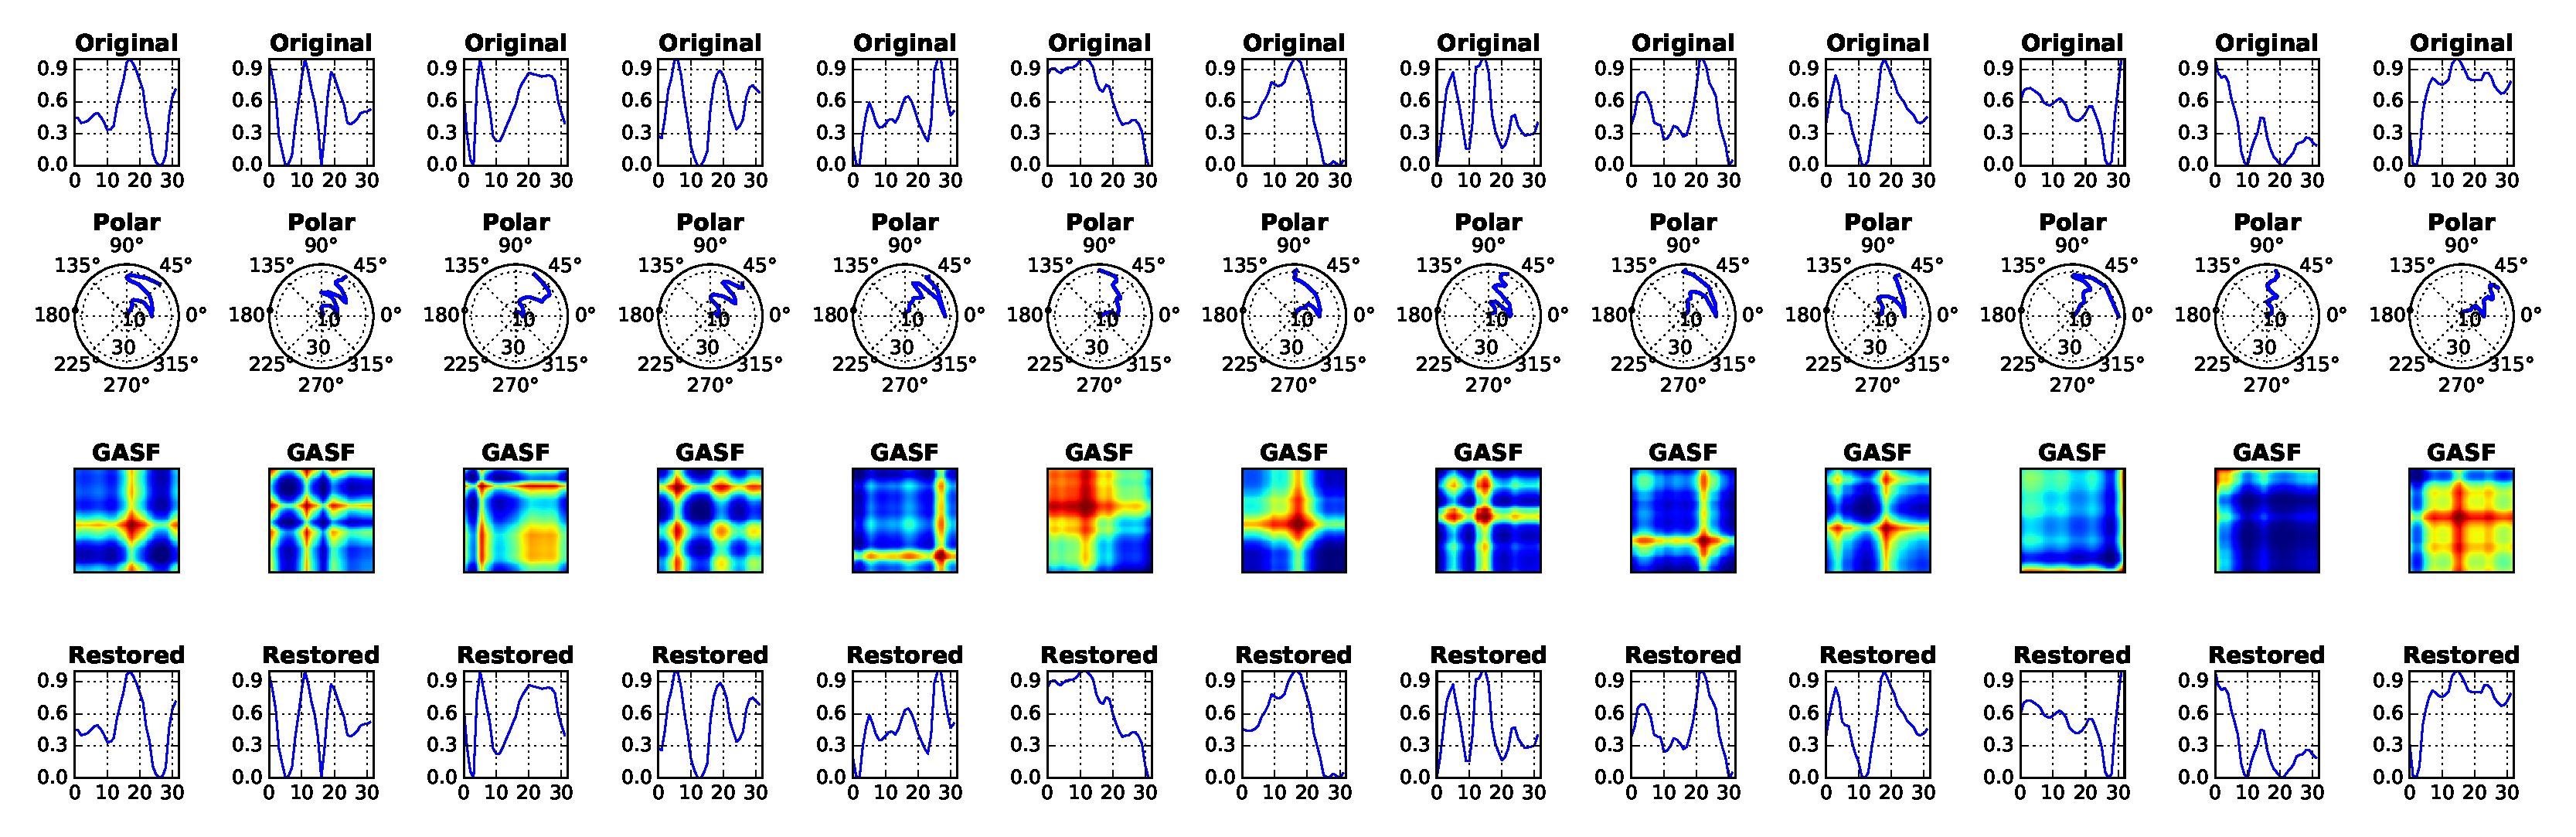
\includegraphics[width=.88\textwidth]{images/05-modeling/gasfpipeline.eps} 
 \caption{Conversion of time series into a Gramian Angular Summation Field (GASF) image and then back into its original space.}
 \label{figure:gasf_example}
\end{figure}

\subsubsection{Latent Dirichlet Allocation}
LDA is one of the most simple and influential topic models. {A topic model is a formal statistical relationship between a group of observed and latent (unknown) random variables, which specifies a probabilistic procedure to generate topics. The latter, in turn, is defined as a probability distribution over a collection of words}~\cite{reed_latent_2012}.

The graphical model shown in Figure~\ref{fig:graphical-model} presents the structure of the \gls{lda} model~\cite{blei_latent_2003}. Here, as in~\cite{smith_mining_2016}, the \textit{K}-th probability distribution over input words $\beta$ (called topics) is representative of the $K$ groups (types) of player motion styles in which we are interested. In turn, each document $d$ corresponds to a {game play} session for the game. We had to deal with the deterioration of model accuracy when considering the whole game section as a single document. Our solution for the problem was to segment each game section into subsets based on duration in seconds. %ANDY I cannot understand why couldn't be partitioned in subsets corresponding to the motion primitive, which already solved the problem. I'm losing my mind.
This approach raises several issues that are going to be properly addressed in a future work, but still allow one to obtain interesting~results. %ANDY This cannot be left like this. It is too open and undefined.

%\begin{figure}[H]
  \centering
  \begin{tikzpicture}
    [
      observed/.style={minimum size=15pt,circle,draw=blue!50,fill=blue!20},
      unobserved/.style={minimum size=15pt,circle,draw},
      hyper/.style={minimum size=1pt,circle,fill=black},
      post/.style={->,>=stealth',semithick},
    ]

    \node (w-j) [observed] at (0,0) {$w_{d,n}$};
    \node (z-j) [unobserved] at (-1.5,0) {$z_{d,n}$};
    \node (z-prior) [unobserved] at (-3,0) {$\theta_d$};
    \node (z-hyper) [label=above:$\alpha$] at (-4.5,0) {};
    \node (w-hyper) [unobserved] at (2,0) {$\beta_k$};
    \filldraw [black] (-4.5,0) circle (3pt);
    
    \node (eta-hyper) [label=above:$\eta$] at (3.5,0) {};
    \filldraw [black] (3.5, 0) circle (3pt);
    
    \path
    (z-j) edge [post] (w-j)
    
    (z-hyper) edge [post] (z-prior)
    (z-prior) edge [post] (z-j)

    (w-hyper) edge [post] (w-j)
    (eta-hyper) edge [post] (w-hyper)
    ;

    \node [draw,fit=(w-j) (z-prior), inner sep=14pt] (plate-context) {};
    \node [above right] at (plate-context.south west) {$D$};
    \node [draw,fit=(w-j) (z-j), inner sep=10pt] (plate-token) {};
    \node [above right] at (plate-token.south west) {$N$};
    \node [draw,fit=(w-hyper), inner sep=10pt] (plate-topic) {};
    \node [above right] at (plate-topic.south west) {$K$};
  \end{tikzpicture}
  \caption{LDA model diagram~\cite{blei_latent_2003}. Each word $w_{d,n}$ corresponds to a window of data from the accelerometer attached to the player during gameplay. In turn, a gameplay is interpreted as a document d (set of player generated words). $z_{d,n}$, represents the type (topic) assignment for a given word $w_{d,n}$ and $\theta_{d}$ is the mixture proportions representing the game session. In this work we are interested in representing the player game session by $\theta_{d}$.}
  \label{fig:graphical-model}
\end{figure}
%ANDY All the terms have to be defined. What is d? What are mixture proportions? What is D?
In these terms, a document may present multiple types $\beta_{k}$ with mixture proportions $\theta_{d}$ The mixture of proportions defines a player at each instant of time. The choice of the $N_{D}$ words comes from $\overline{\beta}_{d}$, which acts as the weighted average of the game play types for a given document. This average is defined as follows~\cite{blei_latent_2003,smith_mining_2016}:

\begin{equation}
\overline{\beta}_{d} = \sum_{n=1}^{K} \theta_{d}(k) \cdot \beta_{k}
\end{equation}

The \textit{n}-th word $w_{d,n}$ of document \textit{d} is, in our case, the GASF encoding obtained, as we will explain later. $z_{d,n} \in \{1:K\}$ refers to the random type from which a word is drawn. Following the standard \gls{lda} model, $\alpha$ and $\eta$ are hyperparameters that control the sparsity in the mixture proportions and word distributions~\cite{smith_mining_2016}.

\subsubsection{Autoencoder}\label{section:autoencoder}

In many problems, we may have to deal with highly dimensional data that represent the situation of the world as captured by the sensors. Given that the raw data dimensionality could be practically intractable, the common procedure in these cases is to reduce the dimensionality possibly keeping only the important features of the input data.

In image processing, for instance, understanding which pieces of an image represent a significant aspect for the task ahead is not a trivial issue. Significance may be related to specific parts of the image and may depend on many aspects. A common technique to face this issue is {autoencoder}.
Autoencoder is an unsupervised learning technique that learns a representation of the input data, usually derived by means of non-linear transformations of the input~\cite{goodfellow_deep_2016}.
A typical implementation of autoencoder consists of a feedforward neural network that first encodes the input into a code, the representation, and then reconstructs the input from it by means of a decoder (see Figure~\ref{fig:autoencoder_architecture}).

\begin{figure}[H]
\centering
\includegraphics[width=.9\columnwidth]{images/05-modeling/autoencoder_architecture}
\caption[Autoencoder general architecture]{General architecture of an autoencoder; the input layer is processed by an encoder that transforms it. The derived representation is then decoded by a decoder that yields a reconstruction.}
\label{fig:autoencoder_architecture}
\end{figure}

In general, autoencoders are good at capturing the structure of the input and tend to represent it well~\cite{goodfellow_deep_2016}. We can represent an autoencoder as a neural network that tries to copy its input to its output. We can represent its general architecture with the following terminology:
\begin{itemize}[leftmargin=*,labelsep=5.8mm]
	\item the input $x$,
  \item the {encoder function}, $f(x)$, composed of some hidden layers,
  \item the {code}, or internal representation, of the input $h$,
  \item the {decoder function}, $g(x)$, composed of other hidden layers,
  \item the reconstruction obtained from the decoder, $r$.
\end{itemize}

A {loss function}, $L(x, r)$, should also be defined to evaluate how close the reconstruction is with respect to the input.
A simple loss function is shown as Equation \eqref{eq:loss_autoencoder}.

\begin{equation} \label{eq:loss_autoencoder}
L(x,r) = \sum_{i} (x_i - r_i)^2
\end{equation}

However, if we do not impose any restriction, the transformation it learns would be an identity, since this would perfectly reconstruct the input. To prevent this transformation, two approaches have been devised~\cite{goodfellow_deep_2016}.
The first, called {undercomplete autoencoder}, adopts a representation smaller than the input (see Figure \ref{fig:under_over_autoencoder}a),
while the latter, {overcomplete autoencoder}, uses a representation with a dimension larger than the input (see Figure \ref{fig:under_over_autoencoder}b).
Although increasing the representation size is counterintuitive in order to sparsely represent the input, this technique has proven its effectiveness.

\begin{figure}[H]
\centering
\begin{subfigure}[H]{0.3\textwidth}
\centering
\includegraphics[width=0.9\textwidth]{images/05-modeling/undercomplete_autoencoder}
\caption{}
\label{figure:undercomplete}
\end{subfigure}
\begin{subfigure}[H]{0.3\textwidth}
\centering
\includegraphics[width=0.9\textwidth]{images/05-modeling/overcomplete_autoencoder}
\caption{}
\label{figure:overcomplete}
\end{subfigure}  \vspace{-6pt}
\caption{(\textbf{a}) Representation of an undercomplete autoencoder, where the representation has a lower dimension with respect to the input. (\textbf{b}) Representation of an overcomplete autoencoder, which uses a larger space to represent the input.}
\label{fig:under_over_autoencoder}
\end{figure}

The undercomplete autoencoder is the oldest and best known architecture for the autoencoder and also the one we use in our work. The code the autoencoder derives is smaller than the input: it learns how to combine the input so that the relevant information is retained in a lower dimensional space. The combination is often non-linear due to a non-linear activation function of the neurons. On~the other hand, the decoder function learns how to unroll such compressed code in order to obtain an extended representation. This architecture could be trained using the classic back-propagation approach, although different methods are available~\cite{goodfellow_deep_2016}.

The overcomplete autoencoder, instead, increases the dimension of the representation; however, as already mentioned, the model could easily learn the identity transformation. In order to tackle this issue, the common approach is to apply a regularization term over the weights of the network. In general, a $l_1$ penalization is added to the loss function.
In this way, the representation will be sparse since some of the dimensions are set to zero.
However, this new architecture would be more complex to train since the model would be larger than the previous one, although still providing a sparse representation.
Despite its sparsity, this architecture is able to extract more information from the input, and it is often used to capture also the input distribution and not just the structure of $x$. It is not possible to estimate such a distribution with an undercomplete autoencoder since such a task would require a higher representation capacity.

In this work, we adopt an undercomplete autoencoder, since our goal is to represent an image in a lower dimensional space. 
Our architecture has multiple layers: the first layer takes only the input, while the following ones decrease in size with the power of two.
We represent the input with a code having 64 dimensions; thus, from an input of 1024 features, we derive a representation of 64 components using an autoencoder.

The reconstruction of the input by the decoder function has a very low loss, below 0.05$\%$. The~layers obtained by the encoder are often difficult to understand by people; for instance, in Figure~\ref{fig:levels_autoencoder}a--c, we can observe the first layer, and we cannot derive any structure or meaning from it.
However, looking at deeper levels, the layers show a clear structure; in Figure~\ref{fig:levels_autoencoder}g--i, we can observe that the filters are extracting horizontal and vertical patterns. Indeed, most of the original images show a cross pattern, or multiple crosses; therefore, this representation seems to be able to represent the input data with a lower dimension.

\begin{figure}[H]
\centering
\begin{tabular}{ccc}
\includegraphics[width=0.2\columnwidth]{images/05-modeling/autoencoder_levels/autoencoders_2_0} &
\includegraphics[width=0.2\columnwidth]{images/05-modeling/autoencoder_levels/autoencoders_2_1} &
\includegraphics[width=0.2\columnwidth]{images/05-modeling/autoencoder_levels/autoencoders_2_2} \\
(\textbf{a}) & (\textbf{b}) & (\textbf{c}) \\
\includegraphics[width=0.2\columnwidth]{images/05-modeling/autoencoder_levels/autoencoders_4_0} &
\includegraphics[width=0.2\columnwidth]{images/05-modeling/autoencoder_levels/autoencoders_4_1} &
\includegraphics[width=0.2\columnwidth]{images/05-modeling/autoencoder_levels/autoencoders_4_2} \\
(\textbf{d}) & (\textbf{e}) & (\textbf{f}) \\
\includegraphics[width=0.2\columnwidth]{images/05-modeling/autoencoder_levels/autoencoders_7_0} &
\includegraphics[width=0.2\columnwidth]{images/05-modeling/autoencoder_levels/autoencoders_7_1} &
\includegraphics[width=0.2\columnwidth]{images/05-modeling/autoencoder_levels/autoencoders_7_2} \\
(\textbf{g}) & (\textbf{h}) & (\textbf{i}) \\
\end{tabular}
\caption{Example layers from the trained autoencoder. (\textbf{a}--\textbf{c}) represent the information extracted by the first layer of the autoencoder. It is hard to grasp the meaning of the representation derived. Going deeper, in (\textbf{d}--\textbf{f}), the representation seems to become more clear and with a structure. Indeed going directly to the obtained code, in (\textbf{g}--\textbf{i}), we can see a more accentuate structure composed mainly of horizontal or vertical lines.}
\label{fig:levels_autoencoder}
\end{figure}

\subsection{Problem Statement} %ANDY this section seems fundational, an probably should stay at the beginning ofthe chapter. Frmulating a problem is typically done before than proposing solutions.
This section formulates the problem of modeling the player as a probabilistic mixture of player styles derived from data. There are at least three basic dimensions (or problems) of interest that must be considered when building a model of this kind for \gls{pirg}s. Such dimensions are related to the specific capabilities of a mobile robot to achieve a suitable in-game performance. We delineate such dimensions as follows:

\begin{itemize}[leftmargin=*,labelsep=5.8mm]
\item {Dimension \#1: Fundamental robot behavior}, which concerns the fundamental aspects of the robot locomotion, timing of actions, localization and other abilities to keep it alive and well-functioning during the game play.
\item {Dimension \#2: In-game competitive capabilities}, which are more related to the intelligent selection of actions aimed at achieving in-game goals. In other words, this dimension captures the intricacies of planning and rational behavior, using solutions developed for Dimension \#1.
\item {Dimension \#3: Adaptive power}, which is a higher level dimension concerned with how and when during the game to adjust the robot performance to match that of the current player.
\end{itemize}

Dimension \#1 concerns the setup of an appropriate robotic platform, including aspects like: electrical disturbances, power consumption, kinematic constraints, processing capabilities, sensing and safety. These are recurrent issues that must be appropriately dealt with. 

Dimension \#2 encompasses the problem of finding a plan or strategy to achieve the robot goals. This is the problem most related to the competitive behavior the robot can impose on the human player, since action selection is driven by the tendency to maximize the robot's own pay-off. After all, the robot has to give the idea that it is at best trying to beat/help its opponent(s)/companion(s).

Dimension \#3, based on \#1 and \#2, defines constraints on the robot behavior such that the action selection is not longer just governed by the tendency to be competitive/helpful, but is also driven by the compelling necessity to support the player interaction, in real time, as robustly as possible.

One can see that the present work as a step towards advancements in Dimension \#3.
%ANDY All this would be nice in the introduction of this thesis, and could drive the presentation, showing as you have faced all these aspects, producing innovative results in some of them. Player modeling is missing here, and could go in \#3, being \#1 dedicated to development of a fully funcyional body, \#2 to the ability to play, and act according the rules, including the ability to aim at winning, descpite the player, while \#3 considers also the player, models it, and try to optimize entertainment more than performance in the game, eventually reducing the robot's abilities. Your main contribution is, of course on \#3, but you had to face also the other two, and, actually, you have to describe them UP to now you haeve described \#1 and part of \#3. #2 is missing at this point, but surely will be in the following.

Here, we exploit data coming from a single accelerometer placed on the human player's body; thus, player movement is our primary source of information for describing the playing style and engagement. 
%ANDY However you have also mentioned IC, and other image-based features. You should take a definite line, putting in evidence clearly what you have explored and then left and whatis teh content of the final proposal, which, BTW, seemed to be based on lasers only, losing the richness provided by the other data sources (accelerometer and Kinect) and the possibility to explore and exploit data fusion.

The basic assumption is that a highly active player would naturally express his/her status by a very turbulent motion signal that is compatible with strong in-game activity. Consider, for instance, the difference in signal shapes reported in Figure~\ref{figure:acc_signal_shape}.

Following this line of reasoning, we also assume players do not fake their engagement by unnecessarily performing strong activities, like running, when they are actually not engaged in the game or feel bored by the robot behavior. Therefore, we assume that a highly motivated player would act more intensively and frequently than a non-motivated one, thus showing a more turbulent acceleration signal profile.

In situations like \gls{pirg}, movement information is useful and should not be disregarded. Furthermore, a model that is able to extract a description of the player's movement profile for the purpose of robot behavior adaptation would generate interesting dynamics able to hide existing platform limitations (kinematics constraints, tracking problems, etc.) and boost game experience.

One important aspect not considered yet by our assumptions is the role of skill level. For example, a highly skilled player could try to minimize his/her energy expenditure by performing precise movements towards winning the game and in theory could perfectly show a low-movement profile. Moreover, these assumptions cannot directly measure player engagement in the game, given that it is also possible for a player to move not too much, but, at the same time, be highly engaged. 

In summary, we are interested in investigating time series data, especially acceleration patterns as proxy and/or engagement cues (given the mentioned assumptions) towards the creation of auto-adjusting robotic companions or opponents.

%ANDY The last 4 paragraphs present nice ideas, but they seem unrelated to each other, just put here as they come to the mind. These considerations are good for the introduction, and the conclusion chapters, and should be integrated with their developments throughout the text.




\begin{figure}[H]
\centering
\begin{subfigure}[H]{\textwidth}
\centering
\includegraphics[width=0.2\textwidth]{images/05-modeling/enricorun.png} 
\includegraphics[width=0.6\textwidth]{images/05-modeling/running_sig_profile.eps} 
\caption{}
\end{subfigure}

\begin{subfigure}[H]{\textwidth}
\centering
\includegraphics[width=0.2\textwidth]{images/05-modeling/enricostill.png}
\includegraphics[width=0.6\textwidth]{images/05-modeling/standing_sig_profile.eps} 
\caption{}
\end{subfigure} \vspace{-6pt}
\caption{Three-axis accelerometer signal during game play. (\textbf{a}) A running player. (\textbf{b}) A player standing still. Notice that signal shape and amplitude are very characteristic for the respective activity.}
\label{figure:acc_signal_shape}
\end{figure} \unskip

\begin{figure}[H]
\centering
\begin{subfigure}[H]{\textwidth}
\centering
\includegraphics[width=0.6\textwidth]{images/05-modeling/example_signal.eps}
\label{figure:accelerometer_signal}
\caption{}
\end{subfigure} \vspace{-6pt}

\begin{subfigure}[H]{\textwidth}
\centering
\includegraphics[width=0.45\textwidth]{images/05-modeling/example_gafs_seg.eps}
\caption{}
\end{subfigure} \vspace{-6pt}
\caption{Example of the conversion of a time series into GASF images. (\textbf{a}) Three-axis accelerometer data (48.8 Hz) of about 30 seconds of real game play. (\textbf{b}) Thirty five GASF segments of a linear combination of the multidimensional time series. Each window comprises 0.65 seconds with 32 samples.}
\label{figure:acc_signal_gasfs}
\end{figure}


\subsection{Activity modeling}
This section describes our approach to model the activity of the player, while emphasizing the differences and similarities with respect to existing methods. We take inspiration from approaches like~\cite{smith_mining_2016, wang_encoding_2015, wang_imaging_2015} and aim at modeling game sessions as ``documents'', where player's acceleration data are considered as ``words''. We use LDA~\cite{blei_latent_2003} to categorize the player's motion profile as a composition or mixture of game play motion types, the latter being analogous to the ``topics'' in the general application of \gls{lda} for document modeling.

Differently from~\cite{smith_mining_2016}, our input word atoms are not discrete. Instead, they are continuous (acceleration data) and also are not attached to any explicit meaning. Take, for instance, the natural interpretability of joystick input signals like ``left'' and ``right'', which convey their respective meaning when controlling a game character, and compare it with an acceleration signal that carries no obvious absolute meaning.

The method adopted for selecting the input words is based on sliding windows (just as in~\cite{smith_mining_2016}), without overlap. %ANDY This choice should be justified, even more since few sections above you discussed the sliding window concept and adopted a different criterion.

Considering each game session as a document, the windowed segments play the role of words. Since the space is continuous, a procedure of discretization and dictionary learning for \gls{lda} had to be performed. For this, we clustered the segments and used the so-obtained cluster centroids as dictionary words.

We have used GASF images instead of GADF because the mapping functions of the rescaled time series in $[\,0,1]\,$ are bijections, which allows for precise reconstruction of the original time series~\cite{wang_imaging_2015}. The reconstruction takes advantage of the the main diagonal of GASF, i.e., $\{G_{ii}\} = \{\cos{2\phi_{i}}\}$, and is performed as reported in Equation~(\ref{equation:reconstruction})~\cite{wang_imaging_2015}: 
%%Please note that the citation of figures should be in numerical order, figure 8 appeared before figure 7, please revise.
\begin{equation}\label{equation:reconstruction}
\cos(\phi)=\sqrt{\frac{G_{ii}+1}{2}} \qquad \phi \in [\,0,\frac{\pi}{2}]\,
\end{equation}

An example of signal decomposition into GASF images is shown in Figure~\ref{figure:acc_signal_gasfs}. Given recent advances in deep learning and pattern recognition for images, we take the route of~\cite{wang_encoding_2015} and exploit the applicability of autoencoders for extracting unsupervised features from GASF images (see Section~\ref{section:autoencoder}). This is relevant since the process of feature engineering is time-consuming and laborious. Moreover, unsupervised feature extraction from such methods has been proven to work well~\cite{wang_imaging_2015, wang_time_2016}.
Sparse encoding via linear-algebra methods for dictionary learning is also a possibility. However, in our experiments, it turned out to be not as efficient as autoencoders. We present details of our experimental activity in the next section. Our methodology is summarized in {Figure~\ref{diagram:methodology}.

%\begin{figure}[H]
%	\centering
%\begin{tikzpicture}[auto]
%	\tikzstyle{b} = [rectangle, draw, fill=blue!20, node distance=0.5cm, text width=4em, text centered, rounded corners, minimum height=5em, thick]
% \tikzstyle{c} = [rectangle, draw, inner sep=0.2cm, dashed]
% \tikzstyle{l} = [draw, -latex',thick]
%
%  \node [b] (time series) {Game time series};
%  \node [b, right=of time series] (segments) {Segments};
%  \node [b, right=of segments] (gasfs) {GASFs};
%	\node [b, right=of gasfs] (features) {GASFs features};
%  \node [b, right=of features] (dict) {Dict. Learning};
%  \node [b, right=of dict] (lda) {LDA};
%
%  \path [l] (time series) -- (segments);
%  \path [l] (segments) -- (gasfs);
%  \path [l] (gasfs) -- (features);
%  \path [l] (features) -- (dict);
%  \path [l] (dict) -- (lda);
%\end{tikzpicture}
%\caption{The general diagram for our methodology. At first, game time series are extracted, which are then segmented into windows (sliding windows method). Such segments are then turned into GASF images, whose representations are obtained using the autoencoder. Since the basic \gls{lda} method works with a multinomial distribution at the topics, we define a dictionary of visual words before feeding each GASF feature document representation to it.}
%\label{diagram:methodology}
%\end{figure}

\subsection{Experimental Results}
In this section, the exploration of an incomplete representation of the GASF images using a simple autoencoder architecture is firstly reported, then we discuss how we transform the extracted features into input words for the \gls{lda} model. Finally, we show the results when confronting the model output with human judgment. All experimental code used is available at the link in supplementary materials. %ANDY Check that this is actually available and report the link here

\subsubsection{Feature Extraction}

The first question we need to answer concerns the size of the sliding window. This parameter regards the definition of the GASF images used as building blocks for the dictionary learning. The~window size should be large enough to capture motion patterns relevant for the player characterization, but not so large to confound their interpretation. We tried different window sizes, and in the end, we followed~\cite{oliveira_activity_2017} and decided to consider half a second of data per window without overlap, which allows for a quite fine-grained data representation.

We applied no preprocessing to the signal, since we were interested in observing how an autoencoder would perform using the unfiltered input. The expectation was that it would naturally compensate for the differences in the images, decisively choosing to capture important features (the main signal characteristic) and disregarding non-representative ones (the small associated noise). We defined an architecture composed by dropout and dense layers where only hyperbolic tangent activation functions where used, except in the last layer, where a linear activation function was used instead. The best performing architecture was composed by the following layers: dropout (0.1 drop fraction), dense (size = 256), dropout (0.2) and dense (size = 64). The same layers (in reversed order) were used for the decoder part.

A window of half a second corresponds to 32 samples given our accelerometer average frequency of 48.8 Hz. As a consequence, we obtain GASF images (without using PAA) with a total of 1024 pixels. Using the autoencoder, we manage to reduce the representation down to a 64-dimensional input, resulting in the reconstruction presented in Figure~\ref{figure:reconstruction}. The choice of a 64-dimensional representation is empirical, meaning that we were in principle searching for an incomplete representation of the data and, upon testing with different configurations, we have chosen the one with the lowest reconstruction error. As it turned out, a 64-dimensional vector representation was the best result, given our dataset. 

\begin{figure}[H]
	\centering
	\includegraphics[width=.9\textwidth]{images/05-modeling/reconstructions.eps}
	\caption{Autoencoder reconstruction for five input segments corresponding to half a second of data (linear combination of the acceleration axis). ({Top line}) Input GASF images. ({Second line}) Original time series for each GASF input. ({Third line}) The autoencoder reconstruction for the input images. ({Forth line}) Time series from the reconstructed GASF images.}
  \label{figure:reconstruction}
\end{figure}

It is possible to notice from the reconstruction result that, despite such a large compression (from 1024 to only 64 values), the input image relevant structure is captured. This can also be seen in the reconstructed time series. A closer look reveals that the autoencoder practically smoothed the time series while preserving the overall shape, this being a nice property that can help to prevent overfitting.

From Figure~\ref{figure:reconstruction}, we can also see that the obtained time series reconstruction presents some holes. This seems to be caused by the information loss in the reconstruction and demands further investigation. However, in our experimentation, it did not seem to affect the learning performance. 

\subsubsection{Dictionary Learning and Input Word Definition}
Latent Dirichlet allocation works by considering the relationship among word tokens with respect to a collection of documents. Therefore, in order to use the method, we needed to come up with a way to encode the taxonomy of GASF images into a discrete set of fixed tokens describing the motion primitives appearing in each game session. We opted to follow~\cite{prince_computer_2012} and encode the features extracted from the GASF using the autoencoders as visual words, composing the game session document.

After getting the 64-dimensional vector representation for each GASF image (see Section~\ref{section:autoencoder}), we cluster them into $V$ groups using the K-means algorithm. In this way, we define a dictionary of size $V$, with each word corresponding to a cluster centroid. Each game session is then translated into a collection of $V$ possible clusters, which can then be fed into the \gls{lda} algorithm.

From text mining and information retrieval, we know that having documents with different sizes can rise critical issues. This is because given the bag of words representation used in \gls{lda}, a small document may be included as a subset in a larger one. Additionally, it might be a problem to evaluate longer documents in our scenario, since, at least from a human perspective, it is not simple to define the overall behavior. %ANDY I'm missing this

In text mining, this issue is handled by imposing a weight based on the length of the document; in our case, instead, we decided to split each session into smaller segments of 15 s each. In this setting, the evaluation is more consistent, and it is possible that the behavior of a player will be maintained within segments. We decided this length for each document both for convenience with respect to the window length and from the assumption that in each fraction of 15 s, the player can show a consistent behavior, which can be somehow easily identifiable. In the next section, we present the results achieved with the approach we just presented.

\subsection{Validation}

Our ultimate objective is to represent the player motion style by a mixture of topic proportions following the \gls{lda} framework. Unfortunately, the method by itself demands the programmer to initialize the desired number of topics. Thus, we had to perform a search for the optimal value given our dataset.

By performing grid search, we selected a range of values for the two main hyperparameters, namely dictionary size, for the input word definition, and number of topics. We would like to keep the number of topics low, preferably less than 10, since by observing our dataset, it is not possible to distinguish many groups of different motion styles; this suggests that a coarse-grained definition would be better. Choosing the number of topics to be at most 10, as in~\cite{smith_mining_2016}, the evaluation of the uncovered topics remains manageable, while maintaining a certain degree of freedom for the existing motion diversity.

The distribution of cluster centroids (words) given topics (our player motion types) is shown in Figure~\ref{overallgame}.
Each line represents a topic, while each column represents a word. As one can see, there are no topics represented by the same distribution over the same word. Figure \ref{overallgame} shows how much each word is important for the specific topic.

\begin{figure}[H]
	\centering
	\includegraphics[width=\textwidth]{images/05-modeling/lda_heatmap.eps}
	\caption{Schematic representation of the game: each line represents a topic, while each column represents a word that is representative of the specific topic.}
  \label{overallgame}
\end{figure}

In order to validate the discovered topics, we use human judgment. We invited volunteers to watch a set of pairs of recorded game segments (15 s each) and point out the similarities between players in their motivation as perceived by their motion. Subjects had to judge how similar, on a scale from 0--5, the movements of two players were. With this, we generated a similarity matrix to be used as the ground truth and main guide for deciding which hyper-parameter value to use and to check whether the proposed method could achieve reasonable results.

The similarity matrix was composed of $406$ independent evaluations from six different human subjects. The generated evaluation matrix was then compared with a cosine similarity matrix generated after training the \gls{lda} in our dataset. The similarity, in this case, is based on the mixture proportions among the discovered topics. 

We used this information to define the number of topics and the number of words. The best set of parameters is the one that presents a higher similarity compared to the one expressing human judgment, thus the smallest Mean Squared Error (MSE). The graph in Figure~\ref{hyperparameter_results} shows the results obtained varying the size of the dictionary (number of cluster centroids) and the number or topics. From it, we have decided to pick 100 as the number of visual words and 10 for the topics present in our dataset.

\begin{figure}[H]
	\centering
	\includegraphics[scale=0.6]{images/05-modeling/mse_dictsize-50_100_10.png}
	\caption{The figure shows the hyperparameter tuning results. The Mean Squared Error (MSE) is estimated with respect to the similarity expressed in the matrix containing the human judgment. The different lines represent the MSE obtained for different dictionary sizes and number of topics.}
  \label{hyperparameter_results}
\end{figure}

The observed similarity results were verified by visual inspection of video logs from estimated similar players; that is, by checking how reported mixture proportions actually look similar in video. However, we state that much work should still be performed towards easily and reliably assessing model correctness and selection. This also relates to the possibility of confidently giving names to discovered motion types, very much in the way as is done in classic \gls{lda} for text categorization.

Another aspect that demands further investigation is how to avoid the decrease in accuracy when considering variable-sized game sessions. As mentioned before, game sessions with different sizes may artificially increase similarity in case one is a subset of another. The solution to this problem provides only a baseline, and much more sophisticated approaches to the problem should be~devised.

We believe that a potential way for improvements in interpretability and accuracy is that of removing the vector quantization in defining each topic. It would be interesting to remain in the continuous domain defined by our input data representation (GASF features), instead of relying on a fixed predefined vocabulary set used for training the \gls{lda}. Such vectorization is known to lead to information loss~\cite{hu_latent_2012}. To avoid such an issue, one possibility may be replacing the topic multinomial distribution by a mixture of Gaussians~\cite{hu_latent_2012}.

\subsection{Discussion}
In this work, we introduced an approach to identify the player motion styles from measurements obtained by the use of a single three-axial accelerometer sensor. Such a signal is then transformed using the Gramian angular field in an image that represents its content. The reason for such representation stems from recent publications aiming at using deep learning and state-of-the-art image processing techniques for achieving better classification results. Additionally, using the autoencoder for representing the obtained GASFs reduced the workload necessary for hand-crafting features, as often done when using machine learning classification/clustering methods with time series data.

By applying latent Dirichlet allocation to characterize the motion behavior of different players, we were interested in getting a description that would foster the development of self-adjusting \gls{pirg}s agents capable of improving/sustaining engagement. In this, we had shown that the model is able to capture the overall human judgment by matching reported similarities. 

This is the first work, to our knowledge, that tries to model the motion behavior of the player using this type of signal in conjunction with \gls{lda} in a robogame scenario. We have demonstrated that the proposed approach is able to cluster and represent different behaviors learned from data. We have evidence that our methodology can achieve better performance than that of relying solely on the measurements of the accelerometer as input for the dictionary learning step. We are still working to provide a fair comparison between the two approaches.%ANDY Another thing to do

As future work, we want to test our approach with a series of different input signals in order to assess its capability. One alternative could be the incorporation of proximity information in order to capture how proximity patterns relate to a player game play style. Moreover, we are interested in measuring the player's effort expenditure in terms of difficulty of motion given a difficult setting for the robot. 

In our method, we also wish to incorporate time dependency. We believe such information would help to describe variations in playing style during play, given the opportunity to detect change points in styles and favor game (robot behavior) personalization. This also may help to avoid the rubber-band effect, a system instability concern often present when designing auto-adjusting game systems.

Another means for improvements, and one that we are currently working on, is that of removing the vector quantization step necessary for the definition of the multinomial distribution of words that defines each topic. We believe that it would be interesting to remain in the continuous domain defined by our input data, instead of relying on a fixed predefined set of tokens, i.e., the vocabulary set used for training the \gls{lda}. Our current experimentation goes along the lines of testing how a Gaussian version of \gls{lda} would work in our domain and whether that could give better results. Additionally, comparing our results with a continuous version of \gls{lda} would help to answer questions regarding {stop word} filtering, such as: To what extent removing certain common segments would improve or worsen accuracy?

Finally, we are working to redesign the experiments in order to allow for collecting user survey data, which comprise a valuable resource regarding player style and engagement levels. This is all in order to increase our understanding of the obtained results. We plan to collect self-reported engagement levels when comparing with different robot behavior configuration while allowing for adaptation. Regarding such adaptation, we currently are investigating how to relate the robot game's difficult settings (such as velocity, tower LED control rules, among others) and the mixture proportion of motion types discovered by our reported method. One alternative is to design a utility function that would describe what is the pay-off in facing a certain player given a certain difficult setting, therefore turning the adaptation problem into a full on-line optimization procedure where we try to match player motion types with robot behavior implied by difficulty settings.

%ANDY Future work has to be cited, however, this is not a paper, but a PhD thesis. Future work related to other parts of the thesis (such as experiments on different behaviors) should take them into account, and experimens should (have) consider(ed) all the aspects to be investigated.

\chapter{Adjusting robot playing behavior through latent skill modeling for increasing player satisfaction}\label{ch:adaptation}

Overleaf link: \url{https://v1.overleaf.com/23518282qswvwgkvmcnr}
\chapter{Using social interaction analysis and deception for entertainment support in a physically interactive robogame}

A game is an activity that one engages in for amusement. In the quest for new playing experiences, robots are being developed to take part in interactive games with humans. Making believable, playing robots able to keep human players engaged and satisfied with the playing experience is the main challenge for this kind of applications. 
With this research aim, this paper investigates the quality of interaction between a human player and a mobile robot in a physical, interactive robogame. We apply previous development in social interaction analysis and, in particular, we focus on the applicability of deception theory as a mean to support engagement. By analyzing the social situation between two players (human and robot), identifying the need for deception, and acting upon it, we aim at decreasing predictability while increasing engagement and amusement, which are related to the perception of an opponent smart enough to compete at the right level. Experiments have been conducted on a population of 93 people which have been asked to play the game and answer a questionnaire. The majority of the participants enjoyed the game and perceived the robot as a rational agent that aims to win the game. Deception was also perceived by most of the players.

\section{Introduction}

As technology grows, the amount of devices that are part of our daily life rises as well. Since childhood, the new generations are learning to interact with technology while playing with new games implemented in embedded systems. This phenomenon can be seen on a large scale with robot games. New researches are made on robots developed to interact with human players in a game environment. Games not only make people have fun, but they are one of the most powerful tools for socialization, and cognitive development~\cite{vygotsky1967play, bruner1976play, piaget2013play}.  While playing competitive games, a person is encouraged to learn the opponent's behavior for various reasons; for example, having a good knowledge of the opponent's behavior is essential for building a winning strategy, and this plays an important role in creating amusement.

%\begin{figure}[htbp]
%\centerline{\includegraphics[width=0.5\columnwidth]{images/06-deception/frontPaper23}}
%\caption{Human-Robot interaction scene from our experiments.}
%\label{fig::front}
%\end{figure}

The main issues that should be faced in this field concern the robot's intelligence as perceived by the human player: low or too high levels may induce the player to leave because the robot is not considered as a valid competitor, and this lowers the entertainment level of the game. 

We are focusing on a challenging type of games, where the players are involved in a physical, quite demanding activity. This type of games has been introduced as Physically Interactive RoboGames (PIRG~\cite{martinoia_physically_2013}). In PIRGs, it is important to model the player, by using the only available data that could describe well enough the movements of the player.

In different and not physical games, deception has been recognized as a way to increase attributions of mental states to the robot\cite{shim2013taxonomy}.

Our research aims at analyzing human-robot interaction in games. More  precisely, we try to improve the study on conflicting games, where the use of intelligent strategies by the players is the main path for winning the game. Deception is one of these strategies and it is not trivial communicating it to a human being using a robot. Our work gives a baseline for detecting and communicating deception in PIRG applications.

% [Andrea] I would not say more than what mentioned above in this section. If we will have space, we could add the following part in the background section.{\color{red}{[LAURA] In \cite{shim2013taxonomy} "Other research shows that robot deceptive behavior can increase users’ engagement in robotic game domains. Work at Yale University [14] illustrated increased engagement with a cheating robot in the context of a rock-paper-scissors game. They proved greater attributions of mental state to the robot by the human players when participants played against the cheating robots. At Carnegie Mellon University [15] a study showed an increase in users’ engagement and enjoyment in a multi-player robotic game in the presence of a deceptive robot referee. By declaring false information to game players about how much players win or lose, they observed whether this behavior affects a human’s general motivation and interest based on the winning frequency, game duration, and so on. These results indicate that deceptive behaviors are potentially beneficial not only in the military domain but also in a human’s everyday context."
% In \cite{shim2013taxonomy} a taxonomy about robot deception is presented; our project could be classified as H-O-P.
To the best of our knowledge, this is the first research work that applies deception theory to support engagement in a PIRG with mobile robotic platforms. 
The paper is organized as follows. Section~\ref{S:RelatedWorks} introduces related works, section~\ref{S:Thegameenvironment} explains in details the game, in section~\ref{S:Method} the method for detecting the need of deception and how to translate it into motion activity are described, experiments and validation of the proposed method are presented in section~\ref{S:Validation}, finally, discussions and conclusions are discussed in sections~\ref{S:Discussion} and~\ref{S:Conclusion}.

\section{Related Works}
\label{S:RelatedWorks}

\subsection{Deception and robots}
Interpersonal situations and interaction between individuals have been studied in sociology. Interdependence theory has been introduced in~\cite{de1980interpersonal}, where the authors studied the fact that people adjust their interactive behavior as consequence of their perception of a social situation. The adjustment is dictated by rewards and costs that every choice in a determinate moment in time can lead to. Every situation, then, can be expressed as a multiple choice of rewards in a matrix form, called outcome matrix. This concept can be seen as an equivalent game theory's normal form game. Furthermore, the authors introduced a four dimensional space where mapping of social situation occur using the constructed outcome matrices. Interdependence, correspondence, control and symmetry are the four dimensions that define that space. The first two respectively represent how much individuals influence each other reward and if outcomes of the individuals are consistent. 
An algorithm for analyzing social situations for robot's interactive behavior that uses the interdependency theory proposed in~\cite{de1980interpersonal}, is described in~\cite{wagner2008analyzing}. Our proposed method takes inspiration as well from~\cite{de1980interpersonal}, but in opposition to~\cite{wagner2008analyzing}, revisits the interdependence space (only 2D space interdependence-correspondence) and the way of mapping the outcome matrices as it will be discussed in Section~\ref{S:Method}.
In~\cite{wagner2009robot} an algorithm for detecting when and whether a robot should deceive has been proposed; the decision is based on the mapping of the outcome matrix to the interdependence-correspondence space. This algorithm has been used in~\cite{wagner2011acting}, where the analysis of the social situation is performed to provide robots with the capacity of determining if deception is needed. 

%MORE INFO: Experiments with the robot that has to choose between 3 paths and it has to deceive in a sense of leaving a false hint of where it passed by; the experiments confirm that outcome matrices can be used for detecting if deception may be needed, but it is focused on other individual's model.
The works of~\cite{de1980interpersonal, wagner2008analyzing, wagner2011acting, wagner2009robot} have laid the foundation for many research activities in social aspects involving humans and robots, in particular on the aspect of \textit{deception}. From the taxonomy in~\cite{shim2013taxonomy}, it is possible to classify deception according to the interaction object. Objectively, there are two types of deception, human-robot and nonhuman-robot.
An example of nonhuman-robot deception is~\cite{shim2012biologically}, where a squirrel-robot was capable of deceiving another one for gaining more food.
On the other hand, deceiving a human is not trivial. Studies about a robot able to deceive a human have been reported in~\cite{terada2010can}, where the authors discuss whether the feeling of being deceived by a robot would be an indicator that the human treats the robot as an intentional entity. 
%MORE INFO: The experiments have been conducted by producing a behavior against the human being's prediction. The robot is only able to rotate on its position for playing 'UN DUE TRE STELLA'. [Andrea] Either we will describe the experiment or I would not mention this.These experiments are not in a playing context.
Further experiments about the engagement increasing in a game due to a robot able to deceive, have been conducted in~\cite{short2010no}. This cheating 'rock-paper-scissors' interactive robot takes advantage of the deception for its own benefit.
%MORE INFO: the robot cheats in the 'rock-paper-scissors' game changing its choice after seeing the opponent's one and changing in its own favor the final result of the game. The authors find that it is noticeable the increased level of engagement by the participants when the robot cheats.
Differently from that robot, the robot presented in~\cite{vazquez2011deceptive} has been programmed for following a multi-player, reaction-time and conflict game, where its main role is to establish who is winning. The robot does not play, but it sometimes changes the wons in order to make the game more social engaging when the players discovered the cheating behavior of the robot. %TODO I can hardly see how the game might become more interesting when cheating of the robot is discovered.
%[EWERTON], this is really strange.

The most important part in a deceiving algorithm is to properly transmit to the deceived the false communication. This is a delicate part because the deceived should not understand it is under deception. 
In~\cite{dragan2014analysis} the authors propose a way to study the communication of false information (deception) using a robotic arm. On the work, the author reinforce the applicability of robot deception in making games against robot more engaging. All the paper is concentrated on robot deception in goal-directed motion, by learning deceptive trajectories in which the robot is concealing its actual goal. The present work is similar to ~\cite{dragan2014analysis} in the sense that it also explores goal-directed motion by following trajectories, but differ from that work on using a full mobile robot in a real game scenario. 

%TODO Actually, this method has not been presented and it seems a completely different context. Let's write what are the similarities.

%[EWERTON] -> improved the description without digging in on the description of the method.

\subsection{Physically Interactive Robogames}

Robot toys are presently the largest amount of robots delivered in our homes, at a rate of millions every year. In almost all the cases, the interaction is limited to stimulus-response reactions, but the introduction of low-cost sensors and computer power are making it possible to introduce a richer interaction and games specifically designed for mobile robots. In a PIRG, physical autonomous (often mobile) agents are actively engaged in a game that creates some sort of interaction, either competitive or cooperative, between humans and robots, moving in the physical world. Robogames will be one of the next robotic products for the mass technological market, thus demanding a large exploration of new methodologies and applications, especially for what concerns methods for enabling high autonomy, intelligence, and adaptive behavior, in order to respond to demands in engagement support like the ones expressed in~\cite{yannakakis_entertainment_2008,yannakakis_how_2008,yannakakis_real-time_2009}. 
Being able to evaluate how people play is crucial for an adaptive game. In the virtual game industry, several studies have been published, most of them using artificial intelligence and machine learning algorithms. For instance,~\cite{drachen_player_2009} reports about emergent self-organizing maps for grouping types of players. 

There have been attempts for presenting robots as toys over the years, where, in most cases, the robot acts more or less like a mobile pet (e.g.,~\cite{fujita_open_1997, brooks_robots_2004}). In these cases, interaction is often seen as limited to almost static positions, not exploiting rich movement, nor high level of autonomy; the credibility of these toys to lively engage people, such as kids, are said to be constrained~\cite{martinoia_physically_2013, bonarini_timing_2014}. 

Some PIRGs have been reported over the last few years. Jedi Trainer 3.0.~\cite{martinoia_physically_2013} was a PIRG mimicking a situation of the first Star Wars saga movie ``Episode IV - A New Hope'': it was able to show some apparent adaptation to the player's playing style as well as some realism of the drone's behavior, which could be understood as some kind of rational behavior by the human player.

Queball~\cite{salter2014designing} was a robotic ball proposed to engage autistic children in games that could have therapeutic goals.

Teo~\cite{bonarini2016huggable} is a huggable, mobile robot designed to play games with autistic children, and to provide the possibility to make free play as well as structuered play experiences.

RoboTower~\cite{oliveira_learning_2017, oliveira_activity_2017, oliveira_modeling_2017}, where humans physically interact with an omni-directional robot by trying to protect towers while avoiding letting the robot pushing them down.
Despite being examples of successful applications, only~\cite{oliveira_learning_2017} and~\cite{oliveira_modeling_2017} present an attempt to quantify the human behavior during gameplay.%for anonymization, while~\cite{oliveira_learning_2017} is the background work for the experiments presented in this paper.

An approach based on genetic algorithms for capturing and modeling individual entertainment is given in~\cite{yannakakis_entertainment_2008}, where the main goal is to construct a player model, in this case a child playing a Playware game. ``Playware is the use of intelligent technology to create the kind of leisure activity we normally label play''%TODO Should this be quoted as it is from the paper?
% [EWERTON] --> Jawohl!
~\cite{lund_playware_2005}. The system can predict the answers to a question asking which variants of the game are more or less ``fun''. In that work, the model is constructed from physiological signals measured during play. 

In summary, pretty much all the related works agree that being able to label player's behavior in a game environment can enable the robotic agent to modify its interactions and playing-style in order to adapt to the skills of its human counterpart. This is a general statement shared with most human-robot interaction applications. On this work, we go further and investigate the introduction of deceptive behavior as another factor for supporting engagement.

\section{The game environment}
\label{S:Thegameenvironment}
\subsection{Playground}
%Omitted for anonymization ---For the present work, we adopt the game environment as follows  described in~\cite{oliveira_activity_2017,oliveira_modeling_2017,oliveira_learning_2017}. 
The playground is a rectangular area of 4 m $\times$ 4 m, where, on each corner, props representing towers are placed. Each tower is equipped with a button and four LEDs that can be progressively turned on. Each tower LED requires the tower button to be pushed without interruption for 2.5~seconds in order to be turned on, meaning that a tower takes about 10~seconds to light up all four of its LEDs. %Such LEDs are used as a representation of the progress of the human player in capturing a specific tower.

After all LEDs of a particular tower are turned on, it is considered as captured by the human player, and the robot will no longer consider it. The activity of turning on LEDs can be distributed in different moments, i.e., the players will not lose their progress if they leave the button before a tower is captured. Tower information such as: tower status (whether active, fallen, or captured) and button presses are transmitted to the robot via wireless communication.

\subsection{Robotic agent}
The robot is a holonomic platform, 70 cm high, 50 cm wide and 50 cm long.
It is capable of navigating autonomously in the environment, using the ROS\footnote{\url{http://www.ros.org}} framework. The robot localization is performed by using Monte Carlo localization algorithms through the AMCL\footnote{\url{http://wiki.ros.org/amcl}.} node, using laser range scans. For the management of sensor information we have implemented custom ROS nodes. By relying on its laser scanners, the robot can also perceive the human player during the game, so as to track her/him, and also to avoid hitting him/her while moving.
Additionally, we also consider the player's distance to towers, extracted from the system  coordinate transformations using the player's position and towers fixed reference frames in the robot's map. 

\subsection{Rules}
In order to win, the human player must be able to secure all the existing towers without letting a single one be knocked down. If, at anytime, a tower falls (because of the robot or player), the game ends, and the human player loses. 

Since the robotic player has holonomic kinematic properties, it is able to move across the entire playground just as the human can and it is only constrained by the fact that an already captured tower, or one whose button is currently being pushed by the player, cannot be teared down. The player can also block the robot path by staying on it. Notice that, while the player is trying to capture a given tower, the robot can try to tear down another one. 

\section{Method}
\label{S:Method}

\subsection{Detecting the need for deception}

During the game, the robot continuously (re)calculates the payoff of attacking (moving closer to) a given tower. For doing that, the robot uses two arrays, $\overrightarrow{t_{robot}}$ and $\overrightarrow{t_{player}}$. The former quantifies the robot's own payoff and the later quantifies the player's payoff. Both payoff are defined by spatial relation. Considering the set of tower positions $\mathcal{T} = \{\tau_{i}\}_{i=1}^{N=4}$, the arrays are defined as in~\ref{eq:array1} and ~\ref{eq:array2}.

\begin{equation}
\overrightarrow{t_{robot}} = \begin{bmatrix}
\delta(\tau_{1},player) -\delta(\tau_{1},robot)  \\ 
\delta(\tau_{2},player) - \delta(\tau_{2},robot)  \\
\delta(\tau_{3},player) - \delta(\tau_{3},robot) \\
\delta(\tau_{4},player) - \delta(\tau_{4},robot)
\end{bmatrix}
\label{eq:array1}
\end{equation}

\begin{equation}
\overrightarrow{t_{player}} = \begin{bmatrix}
\frac{1}{\delta(\tau_{1},robot)} + \frac{1}{\delta(\tau_{1},player)} \\ 
\frac{1}{\delta(\tau_{2},robot)} + \frac{1}{\delta(\tau_{2},player)}  \\
\frac{1}{\delta(\tau_{3},robot)} + \frac{1}{\delta(\tau_{3},player)}  \\
\frac{1}{\delta(\tau_{4},robot)} + \frac{1}{\delta(\tau_{4},player)} 
\end{bmatrix}
\label{eq:array2}
\end{equation}

% \begin{equation}
% target\textunderscore array_{player} = [\forall tower :\frac{1}{\delta_{tower_{i}-robot}} + \frac{1}{\delta_{tower_{i}-player}}]
% \label{eq:array2}
% \end{equation}
Where $\delta(a,b)$ refers to the Euclidean distance between argument $a$ and $b$. Choosing the target tower is done by detecting the maximum value in the arrays:
\begin{equation}
target_{robot} = \operatorname*{arg\,max}_i \, \overrightarrow{t_{robot}}^{(i)}, 
\end{equation}, where $i$ refers to the vector component index.

\begin{equation}
target_{player} = \operatorname*{arg\,max}_i \, \overrightarrow{t_{player}}^{(i)}
\end{equation}

The robot calculates the target preferences for the player as well, in order to be able to predict what would be the opponent's move, as described later.

For recognizing the particular moment in time where deception may be needed, a set of outcome matrices that model the in-game interaction have been defined. Such matrices quantify the payoff, also referred to as utility, associated with each player's actions. As actions, the players can choose to move towards one of the four towers. 

\begin{figure}[htbp]
\centering
\includegraphics[scale=0.35]{images/06-deception/matrix}
\caption{Example of outcome matrix. The columns represent the  robot's payoff in attacking one of the four towers. The rows represent the player's one. Each element is a couple of values, namely the player's payoff and the robot's payoff.}
\label{fig::matrix}
\end{figure}

As the game is a conflicting game, the two players gain benefit in each other's loss. For this reason, the design of the outcome matrices has been made as described here below: the robot earns a higher payoff when itself and the opponent choose a different target. From a matrix point of view, this is seen as a lower payoff in the diagonal elements, because it represents when the two opponents choose the same action.
On the other hand, the player's outcome matrix is built starting from the fact that the human player earns a higher payoff when his/her choice is the same as the robot's one. For this reason, the values of the diagonal elements must be greater than the non-diagonal ones. 

The approach for calculating the robot's outcome matrix is the following:
\begin{itemize}
\item \textit{Non-diagonal Elements:}\\

\begin{equation}
\gamma_r \cdot \frac{\overrightarrow{t_{robot}}^{(i)}}{\sum_{i}{\overrightarrow{t_{robot}}^{(i)}}} \cdot \frac{\delta(\tau_{i},player)}{\sum{\delta(\tau_{i},player)}}, \forall\tau_{i} \in \mathcal{T}\\ 
\end{equation}
, where $\overrightarrow{t_{robot}}^{(i)}$ refers to the component $i$ on the vector $t_{robot}$.
\item \textit{Diagonal Elements:}
\begin{equation}
\delta(\tau_{i},robot)
\end{equation}
Where $\gamma_r$ is a tuning constant. In the robot's outcome matrix, $\gamma_r$ has been used to weight the values of the non-diagonal values, equation (5), while in the player's matrix, another tuning constant has been used for the diagonal values, equation (8). Tuning the values of the outcome matrices is needed for highlighting the fact that the two players win in two different situations. Giving the right value to $\gamma$ is necessary for having a balanced values for the correspondence-interdependence value.
%TODO It is not clear why a tuning is needed, and hwy the two are the same. 
%[LAURA]: tuning is needed for highlighting the fact that the two players win in different situations or it would best saying that the two win with opposite actions (the robot wants to run 'alone' to the tower while the player prefers to have the robot next to him/her so the robot cannot run and win another tower. Giving the right value to gamma is necessary for having a balanced values for the correspondence-interdependence value. They do not have to be the same
The second term in (5) has been used for giving a weight to the payoff: the more an individual is interested in a given target (supposed that this is a consequence of rational~/~maximizer thinking), the higher the payoff is if the player can obtain it.
The third and last term in (5) expresses how much advantage the player has on the other one.
%TODO This explanation is not clear at all. What are the first, second and third terms? It is hard to understand what they are, both because they are in two different equations (numbers could be used to select them
%[ISTEFF] What about refrasing it in "payoff from equation 5 and 7 can be expressed as a multiplication of three terms: the first one etc...
% The first one, \gamma, is a tuning parameter needed for/because of X;
% Payoffs from equations (5) and (7) can be decomposed in a multiplication of two different terms. The first one is the absolute payoff of a given target (%metacomment what I want to say is that this is the payoff not considering the opponent, which is taken into consideration by the next weight) , as it represents the interest of an individual for it given its own state; the second one expresses the advantage the individual has over the opponent to reach the given target, providing a metric of the reachability of the target considering the opponent.
\end{itemize}

Similarly, the player's outcome is described below:
\begin{itemize}
\item \textit{Non-diagonal Elements:}\\
$\forall\tau \in \mathcal{T}$\\
\begin{equation}
 \frac{\overrightarrow{t_{player}}^{(i)}}{\sum_{i}{\overrightarrow{t_{player}}^{(i)}}} \cdot \frac{\delta(\tau_{i},robot)}{\sum_{i}{\delta(\tau_{i},robot)}}, \, \forall\tau_{i} \in \mathcal{T} 
\end{equation}
\item \textit{Diagonal Elements:}
\begin{equation}
\gamma_p \cdot \frac{1}{\delta(\tau_{i},robot)}
\end{equation}
\end{itemize}

From this, a player's utility is periodically (re)computed and then incorporated into the interdependence-correspondence space~\cite{wagner2011acting}.

For our purposes, the \textit{interdependence} dimension represents the correlation between the two players' outcome matrices, while \textit{correspondence} one quantifies how much conflict exists between the two selected actions.

The two values are calculated keeping in mind three concepts: the variation of the robot's outcome matrix resulting from its own decisions; the variation of the player's outcome matrix resulting from the partner's decisions; the variance in outcome matrix resulting from both, joint, interactive decisions.

The calculations for interdependence are made as in algorithm~\ref{alg:interdependence}, where $\alpha \in[-1;0]$, and $\Delta$ expresses the maximum variation the player can obtain on the robot's outcome matrix. The variable \textit{total} expresses the range used for normalization, and $n(\mathcal{T})$ the number of towers.

\begin{algorithm}[h]
\SetAlgoLined
\SetKwInOut{Input}{input}\SetKwInOut{Output}{output}
\Input{Robot's outcome matrix}
\Output{Float value}
\BlankLine
\For{$i \in range(1,n(\mathcal{T}))$ }{
$\Delta_{outcomes} = | max_{outcome(:,i)} - min_{outcome(:,i)} | $ \\
$total = max_{outcome(:,i)} + min_{outcome(:,i)} $\\
$\alpha \mathrel{{+}{=}} \frac{\overrightarrow{t_{robot}}^{(i)}}{\sum_{i}{\overrightarrow{t_{robot}}^{(i)}}} \cdot \frac{\Delta}{total}$
}
\caption{Interdependence algorithm}
\label{alg:interdependence}
\end{algorithm}

The procedure to calculate the correspondence value is defined in algorithm~\ref{alg:correspondence}, where $\beta \in[0;1]$.
\begin{algorithm}[h]
\SetAlgoLined
\SetKwInOut{Input}{input}\SetKwInOut{Output}{output}
\Input{Outcome matrices}
\Output{Float value}
\BlankLine
\textit{Avg(outcome $\forall$ Robot's action)}\\
\textit{Avg(outcome $\forall$ Player's action)}\\

\For{$i \in range(1,n(\mathcal{T}))$}{
\textit{amr = tower index that maximizes robot's outcome} \\
\textit{amp = tower index that maximizes player's outcome} \\
$\Delta_{robot} = outcome_{robot}(amr,i) - outcome_{robot}(amp,i) $ \\
$\Delta_{player} = outcome_{player}(amr,i) - outcome_{player}(amp,i) $ \\
$total_{robot} = outcome_{robot}(amr,i) + outcome_{robot}(amp,i)$ \\
$total_{player} = outcome_{player}(amr,i) + outcome_{player}(amp,i)$ \\
$\beta \mathrel{{+}{=}} \frac{1}{2} \cdot \frac{Avg_{robot}}{\sum{Avg_{robot}}} \cdot \frac{\Delta_{robot}}{total_{robot}} \cdot \frac{\Delta_{player}}{total_{player}}$
}
\For{$i \in range(1,n(\mathcal{T}))$}{
\textit{amr = tower index that maximizes robot's outcome} \\
\textit{amp = tower index that maximizes player's outcome} \\
$\Delta_{robot} = outcome_{robot}(i,amr) - outcome_{robot}(i,amp) $ \\
$\Delta_{player} = outcome_{player}(i,amr) - outcome_{player}(i,amp) $ \\
$total_{robot} = outcome_{robot}(i,amr) + outcome_{robot}(i,amp)$ \\
$total_{player} = outcome_{player}(i,amr) + outcome_{player}(i,amp)$ \\
$\beta \mathrel{{+}{=}} \frac{1}{2} \cdot \frac{Avg_{player}}{\sum{Avg_{player}}} \cdot \frac{\Delta_{robot}}{total_{robot}} \cdot \frac{\Delta_{player}}{total_{player}}$
}
\caption{Correspondence algorithm}
\label{alg:correspondence}
\end{algorithm}
The procedure works by going through every action the robot and the player can take. For example, if the robot decides to take action 1 (go to tower 1), it temporally ignores all the other columns of the robot's outcome matrix and checks what are the indexes that maximize the robot's outcome and the player's one. It then calculates the difference between the outcomes using the two indexes (for both robot and player); a negative $\Delta$ means for the subject that the situation is a conflict (the values of the outcome matrix are positive). The variations are normalized and multiplied by each other and then multiplied by a factor that expresses how likely the action would be taken (if an action will not be chosen, $\beta$ will have a lower impact). Similarly, the same procedure is done w.r.t. the player's actions.

In \textit{Figure~\ref{fig::interdependece}} the correspondence and interdependence space distributions are represented. By making a discretization of the playground into a grid and placing the robot at (4,5), while varying the  player's position on every other coordinate, it is possible to notice that the diagonal that leads to the towers has a higher value of dependency and conflict.

The mapping of the situation to the space shows when deception may be needed. Once an extremely dependent and conflicting situation is detected, deception is triggered.

\begin{figure*}[t]
\centering
\includegraphics[width=\textwidth]{images/06-deception/flowchart}
\caption{The procedure to select deception}
\label{fig:flowchart}
\end{figure*}

Once deception is warranted, the algorithm calculates the fake target to be communicated to the player. The fake target is chosen in the following steps: after the real target is established, the robot calculates two actions that would give the robot the highest rewards and, finally, it calculates which of the two maximizes the player's payoff. This last step expresses the incentive for the player to approach the fake target. The algorithm is detailed in Figure~\ref{fig:flowchart}.

\begin{figure}[H]
\centering
  \begin{subfigure}[t]{0.49\columnwidth}
  \centering
    \includegraphics[width=\linewidth]{images/06-deception/interdependence.jpg}
    \caption{}
    \label{fig:interdipendence}
  \end{subfigure}
  %\hspace{0.01\columnwidth}
  \begin{subfigure}[t]{0.49\columnwidth}
  \centering
    \includegraphics[width=\linewidth]{images/06-deception/correspondence.jpg}
    \caption{}
    \label{fig:correspondence}
  \end{subfigure}
  \caption{Space distribution of the correspondence and interdependence when the robot is placed in (4,5). (a) Interdependence space distribution; darker cells correspond to lower interdependence. (b) Correspondence space distribution; brighter cells indicate lower correspondence.}
  \label{fig::interdependece}
\end{figure}

\subsection{Communicating false goals}
Having presented how to trigger deception, in this section we describe means of effectively using deceptive behavior by communicating false goals, i.e., false attempts to knock down towers. We begin by describing the two methods used.
\subsubsection{Static trajectory approach}
In this first method the trajectories are established a priori. It means that once the navigation node receives the fake and real target information, it calculates, based on the actual position of the robot, the series of points the robot needs to follow in order to communicate the deception.
The algorithm can choose between two different types of trajectories. The first one is activated when the robot is halfway through the fixed frame of localization (map, on the ROS jargon). The robot will then move forward without letting the player know which tower is going to be hit, leaving 50\% of chance of guessing. Only when ``close'', within a predefined threshold, to the midpoint of a virtual line connecting the two towers (true and fake target, respectively), the robot changes trajectory towards the true target.

The second type of deception will try to communicate from the beginning the fake target in order to let the player run and stay to a particular tower, and in this way take spatial advantage when trying to knock down the real target. A pictorially description of such trajectories is shown in Figure~\ref{fig::trajectoryStatic}.

The trajectories are implemented by deciding a series of points to be followed. Those points are spatially distributed along the desired trajectory (Figure \ref{fig::trajectoryStatic}).
% In the first type of deception, the middle point between the two targets is calculated, then three points are extracted in the segment between the robot's position and the middle point. Once reached the third point, the robot changes direction and goes to the real target. %TODO This is different from what shown in the figure.
% Similarly happens in the other type of deception where the subsequent points are calculated between the robot and the fake target, once reached the second or third point of this sequence, the robot changes direction and goes to the real target.

In the present proposal, deception is considered as a complete 'path' that starts when the robot receives the deception information (true and fake tower) and lasts until the robot hits the tower. Since no look-ahead for determining the player position in the future has been considered, it can happen that the player understands the deception and/or the player is really reactive and blocks the robot, so that it would be difficult to finish the deception procedure coherently.
For this reason, the algorithm calculates the time required for successfully making the deception and, every time something goes wrong (for example, the player blocks the robot), the estimated time expires and the deception procedure is aborted. Once it happens, the normal procedure starts again to compute a regular target, until a new need for deception is detected.
\begin{figure}[H]
\centering
  \begin{subfigure}[t]{0.45\columnwidth}
  \centering
    \includegraphics[width=\linewidth]{images/06-deception/trajectoryLaura}
    \caption{Moving forward and then changing the direction.}
    \label{fig:1}
  \end{subfigure}
  \hspace{0.01\columnwidth}
  \begin{subfigure}[t]{0.45\columnwidth}
  \centering
    \includegraphics[width=\linewidth]{images/06-deception/trajectoryLaura2}
    \caption{Moving toward the false target and then changing direction.}
    \label{fig:2}
  \end{subfigure}
  \caption{The two types of deception when using the static trajectory approach.}
  \label{fig::trajectoryStatic}
\end{figure}

\subsubsection{Dynamic steering behavior approach}
The second approach we propose in order to implement a deceiving trajectory is based on steering behaviors~\cite{reynolds1999steering}. The paper by Reynolds proposes a force-based approach to guide an actor in a life-like and improvisational manner. Given a target, it will generate a force, either attractive or repulsive, based on its position with respect to the robot: by applying this force on the robot, it will be driven either towards or away from the target following a smooth path.

Being our robot holonomic, it has been represented as a point mass to calculate the results of the application of the forces generated by the steering behavior. This approach gives us the possibility to dynamically change the robot response to forces by changing the kinematic properties of our representation during the calculation process.

Instead of planning the complete trajectory, only the point where we want to change the motion parameters of the robot and reveal the true target is computed and set as a temporary target. The steering behavior framework drives the robot to reach this target following a slightly different trajectory each time based on its initial velocity and position.

In order to follow a deceptive trajectory as previously described, the dexterity of the robot is dynamically increased when revealing its real target: once the temporary target is reached the virtual mass of the robot is lowered and a higher force is allowed to be applied to it, along with a slight increase on its maximum velocity: then the target to be reached is set to the real target. This procedure generates a sharp turn and an acceleration of the robot towards the real goal. A visualization of the parameter change effect can be seen in Figure~\ref{fig::trajectorySteering}. 

Given this framework, we wanted to investigate whether such change of motion pattern helps the player to realize that the intention carried out by the robot had been to deceive and whether diversity of trajectories increases the appeal of the game by making the robot movements less predictable.

\begin{figure}[htbp]
\centering
\includegraphics[scale=0.33]{images/06-deception/parameterUpdate}
\caption{Update in vehicle parameters and target will produce an increment in robot velocity as well as a smooth bend in the real target direction: on the left we're approaching the temporary target; on the center we change the parameters as we reach the temporary target; on the right we move towards the real target with new parameters}
\label{fig::trajectorySteering}
\end{figure}

%[EWERTON] --> \subsubsection{A machine learning approach} {\color{red} This is going to be used in a follow up project. What about some Journal? YES Social Robotics}

\section{Validation}
\label{S:Validation}
In this section, we describe the acceptability of our strategy within the mentioned interactive scenario. We first present the experimental setup, stating the hypothesis and the use of a post-match survey for evaluating them. The analysis and related discussion follow next. 

%TODO The following sentence was probably left here in editing -> Results from self-report responses to questionnaires filled-up by the participant after each game match.

\subsection{Experimental setup}
\subsubsection{Hypotheses}

\paragraph{H1} The subjects enjoy the game.
\paragraph{H2} The subjects consider the robot as a rational agent, aiming at winning since it is participating to a competitive game.
\paragraph{H3} The two trajectory approaches are both able to create a recognizable level of deception. 
\paragraph{H4} The dynamic steering approach appeals more than the static one.

\subsubsection{Factors}
During our experiments we have kept the parameters that control the general game difficulty discrete such as: maximum speed and maximum acceleration. It was part of our project decision to limit the effect of such variables in this study, while, at the same time, improve safety (since a possible collision against a fast robot is dangerous) and reduce the risk of mechanical problems, since frequent, abrupt acceleration/deceleration might damage the wheel-motor joints.

Speed and acceleration values define two different levels: easy (speed = $0.5m/sec$ and acceleration = $0.1m/sec^2$) and medium (speed = $0.7m/sec$ and acceleration = $0.5m/sec^2$).

However, during experimentation we have noticed that the difficulty level set to easy turned out to be too slow. Therefore, in order to maintain consistency in the analysis while also improving fun we have decided to keep the difficulty fixed at the medium level for all the subjects.

In summary, the only varying factors were the approaches for communicating false goals, i.e., the static trajectory and dynamic steering behavior.

\subsection{Post-Match Survey}

After every match, a questionnaire was administered to each player. It included few questions about the subject (including age and gender) and eleven questions about the game. In this paper, we present results about only four of them, relevant to evaluate the specific hypotheses.

\subsection{Participants}
We recruited 91 participants among the visitors of a science fair. %in Milan held between September 28th and 29th, 2018. 
Most of the experiments were conducted with children, spanning from 5 to 15 years old, while some adults from 16 to 54 years old also accepted to play the game. The distribution of subjects is reported in table~\ref{table::subjectDistribution}. Data collection was performed with subjects being sampled on different times of the day in the attempt to randomize the subjects as best as possible. 

\begin{table}[htbp]
\caption{Gender distribution during the experiments with the static and dynamic trajectory approach.}
\begin{center}
\begin{tabular}{|c|c|c|c|c|}
\hline
\multirow{ 2}{*}{\textbf{Trajectory}} & \textbf{Subject}&\multicolumn{2}{|c|}{\textbf{Gender}} & \multirow{ 2}{*}{\textbf{\textit{Total}}} \\
\cline{3-4}
 & \textbf{Age} & \textbf{\textit{Male}}& \textbf{\textit{Female}} &  \\
\hline
\multirow{ 2}{*}{\textbf{Static}} & Children $(<16)$ & 29 & 19 & 48 \\\cline{2-5}
& Adults $(\geq 16)$ & 6 & 7 & 13 \\
\hline
\hline
\multirow{ 2}{*}{\textbf{Dynamic}} & Children $(<16)$ & 12 & 16 & 28 \\\cline{2-5}
& Adults $(\geq 16)$ & 2 & 0 & 2 \\
\hline
\end{tabular}
\label{table::subjectDistribution}
\end{center}
\end{table}

\begin{figure*}[t]
\centering
  \begin{subfigure}[t]{0.49\columnwidth}
    \centering
    \includegraphics[width=\linewidth]{images/06-deception/staticTooShortYoung}
    \caption{Too short - children.}
    \label{fig::staticTooShortYoung}
  \end{subfigure}
  \hspace{0.01\columnwidth}
  \begin{subfigure}[t]{0.49\columnwidth}
    \centering
    \includegraphics[width=\linewidth]{images/06-deception/staticTooShortAdults}
    \caption{Too short - adults.}
    \label{fig::staticTooShortAdults}
  \end{subfigure}
  %\hspace{0.01\columnwidth}
  \begin{subfigure}[t]{0.49\columnwidth}
  \centering
    \includegraphics[width=\linewidth]{images/06-deception/staticWinYoung}
    \caption{Robot wants win - children.}
    \label{fig::staticWinYoung}
  \end{subfigure} 
  %\hspace{0.01\columnwidth} 
  \begin{subfigure}[t]{0.49\columnwidth}
    \centering
    \includegraphics[width=\linewidth]{images/06-deception/staticWinAdults}
    \caption{Robot wants win - adults.}
    \label{fig::staticWinAdults}
  \end{subfigure}
  %\hspace{0.1\columnwidth}
  \begin{subfigure}[t]{0.49\columnwidth}
  \centering
    \includegraphics[width=\linewidth]{images/06-deception/staticDeceiveYoung}
    \caption{Deception - children.}
    \label{fig::staticDeceiveYoung}
  \end{subfigure} 
  %\hspace{0.01\linewidth} 
  \begin{subfigure}[t]{0.49\columnwidth}
  \centering
    \includegraphics[width=\linewidth]{images/06-deception/staticDeceiveAdults}
    \caption{Deception - adults.}
    \label{fig::staticDeceiveAdults}
  \end{subfigure}
  \caption{Distribution of the agreement with the statement "The game was too short" ((a), (b))."The robot aimed at winning" ((c), (d)). "The robot was deceiving" ((e), (f))  1=Fully disagree 2=Disagree 3=Indifferent 4=Agree 5=Fully agree}
\end{figure*}

\subsection{Results}
All the subjects either agreed or strongly agreed with the statement: "I have enjoyed the game" (median = "strongly agree").

\subsubsection{Static deceiving strategy}
The distribution of the answers to the question: "Was the game too short?" aimed at evaluating the effort to  participate to the game, is reported in Figures~\ref{fig::staticTooShortYoung} and~\ref{fig::staticTooShortAdults}

The distribution of the agreement with the statement: "The robot aimed at winning", aimed at evaluating the perception of playing against a rational agent, is reported in Figures~\ref{fig::staticWinYoung} and~\ref{fig::staticWinAdults}.

The distribution of the agreement with the statement: "The robot was deceiving", aimed at the perception of the deceiving strategy, is reported in Figures~\ref{fig::staticDeceiveYoung} and~\ref{fig::staticDeceiveAdults}.

\subsubsection{Dynamic deceiving strategy}
The number of adult subjects playing with the dynamic deception strategy active was too small to be considered, so we report in this section only data concerning young subjects.

The distribution of the agreement to the statement: "The game was too short" aimed at evaluating the effort to  participate to the game, is reported in Figure~\ref{fig::dynamictooShortYoung}.

\begin{figure*}[tbp]
\centering
  \begin{subfigure}[t]{0.49\columnwidth}
  \centering
    \includegraphics[width=\linewidth]{images/06-deception/dynamicTooShortYoung}
    \caption{Too short.} 
    \label{fig::dynamictooShortYoung}
  \end{subfigure}
  \hspace{0.01\columnwidth}
  \begin{subfigure}[t]{0.49\columnwidth}
  \centering
    \includegraphics[width=\linewidth]{images/06-deception/dynamicWinYoung}
    \caption{Robot wants win.}
    \label{fig::dynamicWinYoung}
  \end{subfigure}
    \hspace{0.01\columnwidth}
  \begin{subfigure}[t]{0.49\columnwidth}
  \centering
    \includegraphics[width=\linewidth]{images/06-deception/dynamicWinYoung}
   \caption{Deception.}
    \label{fig::dynamicDeceiveYoung}
  \end{subfigure}
  \caption{"The game was too short" (subfig a)."The robot aimed at winning" (subfig b). "The robot was deceiving" (subfig c) 1=Fully disagree 2=Disagree 3=Indifferent 4=Agree 5=Fully agree. All subjects were children.}
\end{figure*}

The distribution of the agreement with the statement: "The robot aimed at winning", aimed at evaluating the perception of playing against a rational agent, is reported in Figure~\ref{fig::dynamicWinYoung}.

The distribution of the agreement with the statement: "The robot was deceiving",aimed at the perception of the deceiving strategy, is reported in Figure~\ref{fig::dynamicDeceiveYoung}.

\section{Discussion}
\label{S:Discussion}
We designed a game that obtained a good acceptance by all the participants, most of which queued for participating and were pleased after the game. From the values of the agreement to the statement "I have enjoyed the game", none of which was lower than "Agree", it can be said that hypothesis H1 is satisfied.  

%The length of the game was considered differently by the two classes of players with no big differences w.r.t. the different playing algorithms. It seems that adults had liked a longer play time, while children almost evenly distributed their answers among the five options.

The robot was generally perceived as a rational agent, aiming at winning the game. So we can consider hypothesis H2 as satisfied. This is a good result since the implemented strategies purposefully reduced the capabilities of the robot to adapt its behavior to match those of the players.

Furthermore, deception was perceived by most of the players, with a slightly higher number of subjects among the children strongly agreeing on the fact that the robot was actually deceiving. Hypothesis H3 can also be considered as satisfied.

No significant difference can be detected between the two algorithms in the children population, where it is possible to compare the data, so hypothesis H4 has to be rejected for this sample. Possibly, the difference between the trajectories has been washed out by the quick dynamics of the game, and the high requirement of attention to many different aspects such as the robot movement and position, the position w.r.t. the towers, and the LEDs on the towers.

\subsection{Limitations}
Among the limiting conditions of our work is the lack of a player model that can be used to tailor the deceptive motion on line. For instance, Machine Learning algorithms can be used to model the player's actions and try to maximize the level of surprise~\cite{Baldi_Ittinn} regarding tower attack.
Another limitation comes from constraints that prevent quick changes in motion direction, imposed for safety reasons, which, in turn, may produce negative impacts on the perception of the deceptive movements.

\section{Conclusion and Future Works}
\label{S:Conclusion}
We have implemented a lively, enjoyable, physical robogame, where the robot is perceived as a rational agent aiming at winning the game, even if its capabilities are strongly reduced w.r.t. its possible top performance. This is an example where effective human-robot interaction is obtained by implementing robots that are not behaving optimally, in the sense of minimizing some performance parameter, but they match the expectation of interacting people to attribute rationality to the robot companion, which is one of the aims of human-robot interaction.
This result has been obtained also because of the two different deception algorithms that we have implemented, together with the system that triggers them by analyzing the game situation. These implemented deceptive trajectories are not optimal to win, but obtain the desired effect on the player. 

In the next future, we plan to collect sufficient data to perform sound statistical analyses, and to finalize a system to adapt the behavior and strategy of the robot to the perceived behavior, ability and strategies of the human players, in real time, so to optimize their satisfaction and enjoyment. 
\chapter{Key issues in designing engaging physically interactive robogames}
\chapter{Future work and conclusion}\label{ch:future}

There is a series of future developments for the work we have conducted. In this chapter we try do give an extensive road-map of activities considered worthwhile trying and which are estimated to improve upon the work done. We begin by the futures works related to the~\gls{lda} based approach in chapter~\ref{ch:modeling}.

\section{Latent modeling with~\gls{lda}}
As future work, one alternative could be the incorporation of \textit{proximity} information in order to capture how distance patterns relate to playing style and interest. This measure, similar to what has been done in section~\ref{sec:simple_model}, would them add up to the physical activity description and allow for a fine-grained topic description.

Another opportunity for improvements is in the incorporation of time dependency between the extracted windows. In other words, one would go beyond the \textit{bag-of-words} representation explored by the basic~\gls{lda}. We believe the incorporation of time dependencies would help to describe variations in playing style during play, given the opportunity to detect change points in styles and favor game personalization though robot behavior adaptation. This also may help to avoid the~\gls{rbe}, which is defined as the oscillatory system instability often present when designing auto-adjusting game systems and translates to making the game too easy when too hard and making the game too hard when too easy. This oscillation is a concern since the player would perceive the game as trying to explicitly adjust to his behavior and, thus, have a large impact in player engagement~\citep{martinoia_physically_2013}.

Vector quantization is an standard practice and is used across different applications,~\eg acoustic topic models~\citep{kim_acoustic_2009,kim_audio_2009} and scene understanding~\citep{cao_spatially_2007,li_towards_2009,niu_context_2012}. Here, it is necessary for the definition of the multinomial distribution of words that defines each topic. Despite all, vector quantization for obtaining clusters as word-like units has some drawbacks. Among these are the loss of information and the difficulty in clustering the quantization results coherently, mostly in presence of closely spaced elements in the vector space~\citep{hu_latent_2012}.

We believe that it would be interesting to remain in the continuous domain defined by the feature data, instead of relying on a fixed predefined set of tokens, i.e., the vocabulary set used for training the~\gls{lda}. This open new ways to experiment with the model definition.

One important aspect not considered by our model is the role of skill. For example, a highly skilled player could try to minimize his/her energy expenditure by performing precise movements towards winning the game and in theory could perfectly show a low-movement profile.  The incorporation of such notion can occur by imposing new variables and dependencies between them. 

To the best of our knowledge, our work is the first one to model the motion behavior of the player using raw accelerometer signal in conjunction with~\gls{lda} in a~\gls{pirg} scenario. We have demonstrated that the proposed approach is able to cluster and represent different play types learned from data. Our results indicate the approach is able to approximate well human similarity and is believed to be useful to support player modeling in such situation. We hope further research in the direction of what has been exposed above will provide a definitive proof of the method and better quantify its efficacy. 

\section{Deception}


\section{Skill adaption}


%=============================================
% Bibliography
%---------------------------------------------
\cleardoublepage
\phantomsection
%\printbibliography

%=============================================
% Appendices
%---------------------------------------------

\cleardoublepage
\appendix

%\chapter{Description of the environments}
\label{a:description}

In this appendix we will summarize all the details regarding all the environments used in the experiments of this work.


\section{LQR}
\label{a:lqr_description}
The \glsfirst{lqr} domain is the classical control theory task of stabilizing a linear system (with a linear feedback controller) under a quadratic cost objective function. The system dynamics are:
\begin{equation*}
x(t+1) = Ax(t) + Bu(t).
\end{equation*}
In our experiments we used the identity matrix for $A$ and $B$.
The reward function is:
\begin{equation*}
r(t) = -x(t)^TQx(t) - u(t)^TRu(t).
\end{equation*}
The discount factor for every experiment using this environment is set to $\gamma=0.9$.
This environments has no absorbing states, but we set an horizon of 50 steps for each episode.

\section{NLS}
\label{a:nls_description}
The \gls{nls} environment is a 2D nonlinear system defined in~\cite{vlassis2009learning}.
The system dynamics are:
\begin{align*}
x_1(t+1)&=x_1(t)-0.2\,x_2(t+1)+\eta, \\
x_2(t+1)&=x_2(t)+\dfrac{1}{1+\exp(-u(t))}-0.5+\eta.
\end{align*}
where $\eta\sim\mathcal{N}(0,0.02)$.

The reward function is:

\begin{equation*}
r(t)=\begin{cases}
1 & \left\Vert x\right\Vert <0.1\\
0 & \textit{otherwise}
\end{cases}.
\end{equation*}

The trajectories have an horizon of 80 control steps. The discount factor used in the experiment involving this non linear system is $\gamma=0.95$.

\section{Ship Steering}
\label{a:ship_steering_description}
\begin{table}[b]
  \centering
  \begin{tabular}{c r r}
     \toprule
     Variable & Min & Max \\
     \midrule
     $x$ & 0 & 150 \\ 
     $y$ & 0 & 150 \\
     $\theta$ & $-\pi$ & $\pi$ \\
     $\dot{\theta}$ & $-\frac{\pi}{12}$ & $\frac{\pi}{12}$ \\
     $u$ & $-\frac{\pi}{12}$ & $\frac{\pi}{12}$ \\
     \bottomrule
  \end{tabular}
  \caption{State and action ranges for small and difficult environment}
  \label{tab:ship_steering_small_ranges}
\end{table}

The ship steering problem consist in driving a ship towards a gate. Similar environments have been used both in control theory~\cite{Anderson1990} and reinforcement learning~\cite{ghavamzadeh2003hier}. The state dynamics for the environment is the following:
\begin{eqnarray*}
x(t+1) & = & x(t) + v\sin(\theta(t))dt \\
y(t+1) & = & y(t) + v\cos(\theta(t))dt \\
\theta(t+1) & = & \theta(t) + \omega(t)dt \\
\omega(t+1) & = & \omega(t) + (u - \omega(t))dt/T
\end{eqnarray*}
With $v = 3.0m/s$, $dt = 0.2s$, $T = 5.0$ and $u\in[-\frac{\pi}{12}, \frac{\pi}{12}]$ (radians/s).
The transition model applies the above dynamics for $n$ steps. The reward function is:
\begin{equation*}
r(t)=\begin{cases}
r_{\text{out}} & \textit{outOfBounds}\\
0 & \textit{throughGate}\\
-1 & \textit{otherwise}
\end{cases},
\end{equation*}
where \textit{throughGate} is true if the ship crossed the gate in the last transition, and \textit{outOfBounds} is true if the ship goes out of the environment bounds.
If the ship crosses the gate or goes outside the field, the trajectory ends. The trajectory horizon is set to 5000 control steps. The discount factor used in the experiments on all variants of this environment is $\gamma = 0.99$.

Three different versions of this environment are used in this work: the small environment, the big environment and the difficult environment.
Both the small and the difficult environment share the same state and action space, reported in \cref{tab:ship_steering_small_ranges}. The gate is a line connecting the two points $g_s=(100, 120)$ and $g_e=(120, 100)$.
The difference between these two environments are the reward and the integration steps. In the small environment we have $n=3$ and $r_{\text{out}}=-100$, while in the difficult environment $n=1$ and  $r_{\text{out}}=-10000$.

\begin{table}[t]
	\centering
	\begin{tabular}{c r r}
		\toprule
		Variable & Min & Max \\
		\midrule
		$x$ & 0 & 1000 \\ 
		$y$ & 0 & 1000 \\
		$\theta$ & $-\pi$ & $\pi$ \\
		$\dot{\theta}$ & $-\frac{\pi}{12}$ & $\frac{\pi}{12}$ \\
		$u$ & $-\frac{\pi}{12}$ & $\frac{\pi}{12}$ \\
		\bottomrule
	\end{tabular}
	\caption{State and action ranges for big environment}
	\label{tab:ship_steering_big_ranges}
\end{table}
The state bounds for the ship steering environment are reported in \cref{tab:ship_steering_big_ranges}. The integration steps and the out of bounds penalty for this version of the environment are the same as  the small environments \ie $n=3$ and $r_{\text{out}}=-100$.
\section{Segway}
\label{a:segway_description}
\begin{figure}[b]
	\centering
	\includegraphics{images/env/segway}
	\label{fig:segway_vars}
	\caption{The Segway environment and state variables}
\end{figure}

The Segway is a balancing wheeled robot, that can be described as an inverted pendulum mounted on a wheel, as shown in \cref{fig:segway_vars}. The objective of this environment is to drive the Segway towards the goal position, while maintaining vertical the inverted pendulum as much as possible. This environment is very similar to the Segway described in~\cite{jia2015deep}, however differently from the previous work, we added the position control.
The system dynamics are the following:
\begin{eqnarray*}
\dot{\alpha} & = &\omega_{\alpha} \\
\dot{\beta} & = &\omega_{\beta} \\
\dot{s} & = & -\omega_{\beta}r \\
\dot{\omega_{\alpha}} & = &-\dfrac{h_2 l M_p r\omega_{\alpha}^2\sin\alpha - g h_1 l M_p\sin\alpha + (h_2+h_1)u}{h_1h_3-h_2^2} \\
\dot{\omega_{\beta}} & = &\dfrac{h_3 l M_p r\omega_{\alpha}^2\sin\alpha - g h_2 l M_p\sin\alpha + (h_3+h_2)u}{h_2h_3-h_2^2}\\
h_1 & = & (M_r+M_p)r^2+I_r \\
h_2 & = & M_prl\cos(\alpha) \\
h_3 & = & l^2M_p+I_p.
\end{eqnarray*}
The control action $u$ is constrained such that the applied torque falls in the interval $[-5, 5]$.
The discount factor used in the experiments involving this environment is $\gamma = 0.99$.
The values for the parameters of the system can be found in \cref{tab:segway_parameters}.
\begin{table}[t]
	\centering
	\begin{tabular}{c l}
		\toprule
		Parameter & value\\
		\midrule
		$M_r$ & $0.3*2$ \\
		$Mp$ & $2.55$ \\
		$I_p$ & $2.6\cdot 10^{-2}$ \\
		$I_r$ & $4.54\cdot10^{-4} * 2$ \\
		$l$ & $13.8\cdot 10{-2}$ \\
		$r$ & $5.5\cdot 10^{-2}$ \\
		$dt$ & $10^{-2}$ \\
		$g$ & 9.81 \\
		\bottomrule
	\end{tabular}
	\caption{Parameters used in the Segway environment}
	\label{tab:segway_parameters}
\end{table}

The transition model is obtained by integrating the system dynamics, applying constant torque action $u$, for $\Delta t=0.02$.
The initial state is $x_0=[-1.0, \frac{\pi}{8}, 0, 0]$. 
The discount factor for every experiment using this environment is set to $\gamma=0.9$.
All the states where $\alpha\not\in[-\frac{\pi}{2}, \frac{\pi}{2}]$ or $s\not\in[-2, 2]$ are absorbing states. All trajectories that doesn't reach an absorbing state are cut using an horizon of 1500 control steps.
The reward function is the following: 
\begin{equation*}
	r(t)=\begin{cases}
		-10000 & \textit{fall}\\
		-10000 & \textit{out}\\
		-x(t)Qx(t)^T, & \textit{otherwise}
	\end{cases},
\end{equation*}
where $Q=diag([10, 3, 0.1, 0.1])$ is a diagonal weights matrix for the quadratic cost penalty,  \textit{fall} and \textit{out} are true when the pendulum angle $\alpha$  and the position variable $s$ go outside their bounds.

\section{Prey-Predator}
\label{a:prey_predator_description}
\begin{table}[b]
	\centering
	\begin{tabular}{c r r}
		\toprule
		Variable & Min & Max \\
		\midrule
		$x_{\text{prey, predator}}$ & -5 & 5 \\ 
		$y_{\text{prey, predator}}$ & -5 & 5 \\
		$\theta_{\text{prey, predator}}$ & $-\pi$ & $\pi$ \\
		$v_{\text{prey}}$ & 0 & 1.3 \\
		$v_{\text{predator}}$ & 0 & 1.0 \\
		$\omega_{\text{prey}}$ & -2.1666 & 2.1666 \\
		$\omega_{\text{predator}}$ & -1.666 & 1.666 \\
		\bottomrule
	\end{tabular}
	\caption{State and action ranges for prey-predator environment}
	\label{tab:segway_ranges}
\end{table}
The prey-predator environment consist in two differential drive robots, where the objective of the learning agent, the predator, is to catch the other robot, the prey, inside a square environment with obstacles. Both robots are considered as points, with no footprint.
The prey has a higher maximum angular velocity than the predator but they have the same turning radius ($0.6m$).
The differential drive dynamics used are the following:
\begin{align*}
 x(t+1) & = x(t)+\cos(\theta(t))v(t)dt \\
 y(t+1) & = y(t)+\sin(\theta(t))v(t)dt \\
 \theta(t+1) & = \theta(t)+\omega(t) dt.
\end{align*}
In our experiments we set $dt=0.1$.
State and action are bounded as described in~\cref{tab:segway_ranges}.
The environment is constituted by the following obstacles: the segment $(1, 3.48)-(5, 3.48)$ and the polygonal chain $(-3.0, -1.5)-(-3.0, 1.25)-(-1.48 ,1.25)-(-1.48, -1.5)$. In~\cref{fig:prey_predator_example} a graphical representation of this environment is shown.

The prey is considered captured if the predator distance is less than $0.4m$ and there is no obstacle between the two robots. If the prey has been captured, then the episode ends. All episodes are cut after an horizon of 500 steps.

\begin{figure}[t]
    \centering
    \includegraphics[width=0.5\textwidth]{images/env/prey_predator}
    \caption[The Prey-Predator environment]{The prey-predator environment. Predator is shown in red, prey in blue. The white area around the predator represents the catch radius.}
    \label{fig:prey_predator_example}
\end{figure}


The evasion policy of the prey is a complex policy. The linear velocity is calculated as follows:
\begin{equation*}
v_{\text{prey}}(t)=\begin{cases}
0 & \text{distance} > 3.0\\
1.3 & \text{distance} \leq 1.5\\
0.65 & \textit{otherwise}
\end{cases}
\end{equation*}
To compute the angular velocity, first is computed the difference between the current prey angle and the angle \wrt the predator. then the value of the angular velocity is computed by multiplying the error by a proportional gain $k=\frac{1}{\pi}$. If a potential collision is detected within $1.5m$, the prey rotates in the direction of the biggest angle at maximum angular velocity. If following this rotation, the prey is closer than $0.9m$ to another obstacle, the rotation is inverted. This last behaviour is implemented in order to maneuver properly near the corners, avoiding to get trapped easily.

The reward function for this environment is computed by multiplying by -1 the distance of the prey and the predator after applying the action \ie is computed using the next state. For every experiment using this environment the discount factor is set to $\gamma=0.99$.




\end{document}
